\documentclass[mathserif]{beamer}

\usepackage{grffile}
%\usepackage{natbib}
\usepackage[english]{babel}
\usepackage[latin1]{inputenc}
\usepackage{amsmath,amsthm, amssymb, latexsym,bm}
\usepackage[orientation=landscape,size=a0,scale=0.9,debug]{beamerposter}
% \usepackage[orientation=landscape,size=custom,width=200,height=120,scale=1.9]{beamerposter}
\usepackage{float}
\usepackage{makecell}
%\usepackage{caption,subfig}
\usepackage{tikz}
\usetikzlibrary{matrix,arrows}
\usetikzlibrary{shapes,patterns,snakes}
\usetikzlibrary{positioning,fit,calc}
\usepackage[numbers]{natbib}
%\usepackage{subcaption}
\usepackage{subcaption}
\captionsetup{compatibility=false}
\usepackage{graphicx}


% change list indention level
%\setdefaultleftmargin{3em}{}{}{}{}{}

\setlength{\parindent}{0pt}

%\usepackage{snapshot} % will write a .dep file with all dependencies, allows for easy bundling

\usepackage{array,booktabs,tabularx}
\usepackage{changepage}
\usepackage{setspace}

\usepackage{xcolor}
% \usepackage{float}
% 
\usepackage[colorinlistoftodos,prependcaption,textsize=tiny]{todonotes}
\newcommand{\unsure}[2][1=]{\todo[linecolor=red,backgroundcolor=red!25,bordercolor=red,#1]{#2}}
\newcommand{\change}[2][1=]{\todo[linecolor=blue,backgroundcolor=blue!25,bordercolor=blue,#1]{#2}}
\newcommand{\info}[2][1=]{\todo[linecolor=OliveGreen,backgroundcolor=OliveGreen!25,bordercolor=OliveGreen,#1]{#2}}
\newcommand{\improvement}[2][]{\todo[linecolor=green,backgroundcolor=green!25,bordercolor=green,#1]{#2}}
\newcommand{\thiswillnotshow}[2][1=]{\todo[disable,#1]{#2}}
% \newcommand{\highlight}[1]{\todo[color=yellow,inline]{#1}}
% \usepackage{natbib}
% \setlength{\bibsep}{0.0pt}
\let\oldbibliography\thebibliography
\renewcommand{\thebibliography}[1]{%
  \oldbibliography{#1}%
  \setlength{\itemsep}{-.5ex}%
}

\mode<presentation>{\usetheme{Tufts}}

%\newcolumntype{Z}{>{\centering\arraybackslash}X} % centered tabularx columns
%\newcommand{\pphantom}{\textcolor{ta3aluminium}} % phantom introduces a vertical space in p formatted table columns??!!


\newcommand{\highlight}[1]{{\color{tuftsblue}#1}}
\newcommand\scalemath[2]{\scalebox{#1}{\mbox{\ensuremath{\displaystyle #2}}}}

\listfiles

%%%%%%%%%%%%%%%%%%%%%%%%%%%%%%%%%%%%%%%%%%%%%%%%%%%%%%%%%%%%%%%%%%%%%%%%%%%%%%%%%%%%%%
\graphicspath{{figures/}}
 
\title{\huge Fourier Neural Operators as nonlinear
time-varying system models}
\author{Rad Haghi\footnotemark[1], Bipin Jairaj Gaikwad\footnotemark[1] and Abani Patra \footnotemark[1]{\bf include Babak?}}

\institute[Tufts University]{\footnotemark[1]Tufts Institute for Artificial Intelligence, Tufts University, Medford, MA 02155}
%To change the footer, change it in beamerthemeTufts.tex

%%%%%%%%%%%%%%%%%%%%%%%%%%%%%%%%%%%%%%%%%%%%%%%%%%%%%%%%%%%%%%%%%%%%%%%%%%%%%%%%%%%%%%
\newlength{\columnheight}
%\setlength{\columnheight}{75cm}
% Instead of \setlength{\columnheight}{75cm}
% Try a more flexible approach:
\setlength{\columnheight}{0.85\textheight}

%%%%%%%%%%%%%%%%%%%%%%%%%%%%%%%%%%%%%%%%%%%%%%%%%%%%%%%%%%%%%%%%%%%%%%%%%%%%%%%%%%%%%%
\begin{document}
\begin{frame}
	\begin{columns}

%----------------------------------------------------------Left Column ---------------------------------------------------------------
		\column{.25\textwidth}
		\begin{beamercolorbox}[center,wd=\textwidth]{postercolumn}
			\begin{minipage}[T]{.95\linewidth}  % tweaks the width, makes a new \textwidth
			     \parbox[t][\columnheight]{\textwidth}{ % must be some better way to set the the height, width and textwidth simultaneously
			      % Since all columns are the same length, it is all nice and tidy.  You have to get the height empirically
			
					\begin{block}{Introduction}
%Fourier Neural Operators (FNOs) have emerged as powerful surrogate modeling tools for parametric PDEs and nonlinear dynamical systems \cite{kovachkiNeuralOperatorLearning2024,li2021}. While FNOs have been successfully applied to systems with time-invariant parameters from steady-state problems like Darcy flow to time-dependent flows such as Burgers' and Navier-Stokes equations \cite{kovachkiNeuralOperatorLearning2024}, magnetohydrodynamic plasma evolution \cite{rahmanSparsifiedTimedependentFourier2024}, and multiphase flow simulations \cite{iiModelParallelFourierNeural2023} limited work has explored FNOs for explicitly time-varying parameters. This research addresses this gap by introducing an FNO-based approach for nonlinear time-varying systems, validated using a two-degree-of-freedom Duffing oscillator with evolving stiffness. A key innovation is the integration of a frequency-domain (spectrogram-based) loss function \cite{chakraborty2025, cao2024}, which enhances the model's ability to capture complex dynamics in systems with temporally evolving parameters. In this work, we first present the result of using out of the box FNO on an complex linear system. Then we show how adding the spectrogram loss to FNO improves the prediction significantly. 
Fourier Neural Operators (FNOs) have emerged as effective surrogate models for parametric PDEs and nonlinear dynamical systems \cite{kovachkiNeuralOperatorLearning2024,li2021}. %\todo{unsure about dynamical systems}. 
Recent theory \cite{lantholer24} shows FNO approximation error bounds as a function of grid discretization and solution regularity, also building confidence in the method.
Although FNOs have successfully addressed steady-state and time-dependent systems \cite{kovachkiNeuralOperatorLearning2024,rahmanSparsifiedTimedependentFourier2024,iiModelParallelFourierNeural2023}, few studies have explored complex nonlinearities and explicitly time-varying parameters.  
This research fills this gap by applying FNOs to nonlinear systems with time-dependent parameters, demonstrated on a 2-DOF Duffing oscillator with varying stiffness. A spectrogram-based loss function \cite{chakraborty2025,cao2024} significantly enhances prediction accuracy. Results show that integrating this frequency-domain loss notably improves the FNO's performance.



					\end{block}
			 
					\begin{block}{Fourier Neural Operator}
                    The ``out-of-the-box" FNO architecture \cite{kovachkiNeuralOperatorLearning2024} presented in figure below.
                    \begin{figure}
                        \centering
                        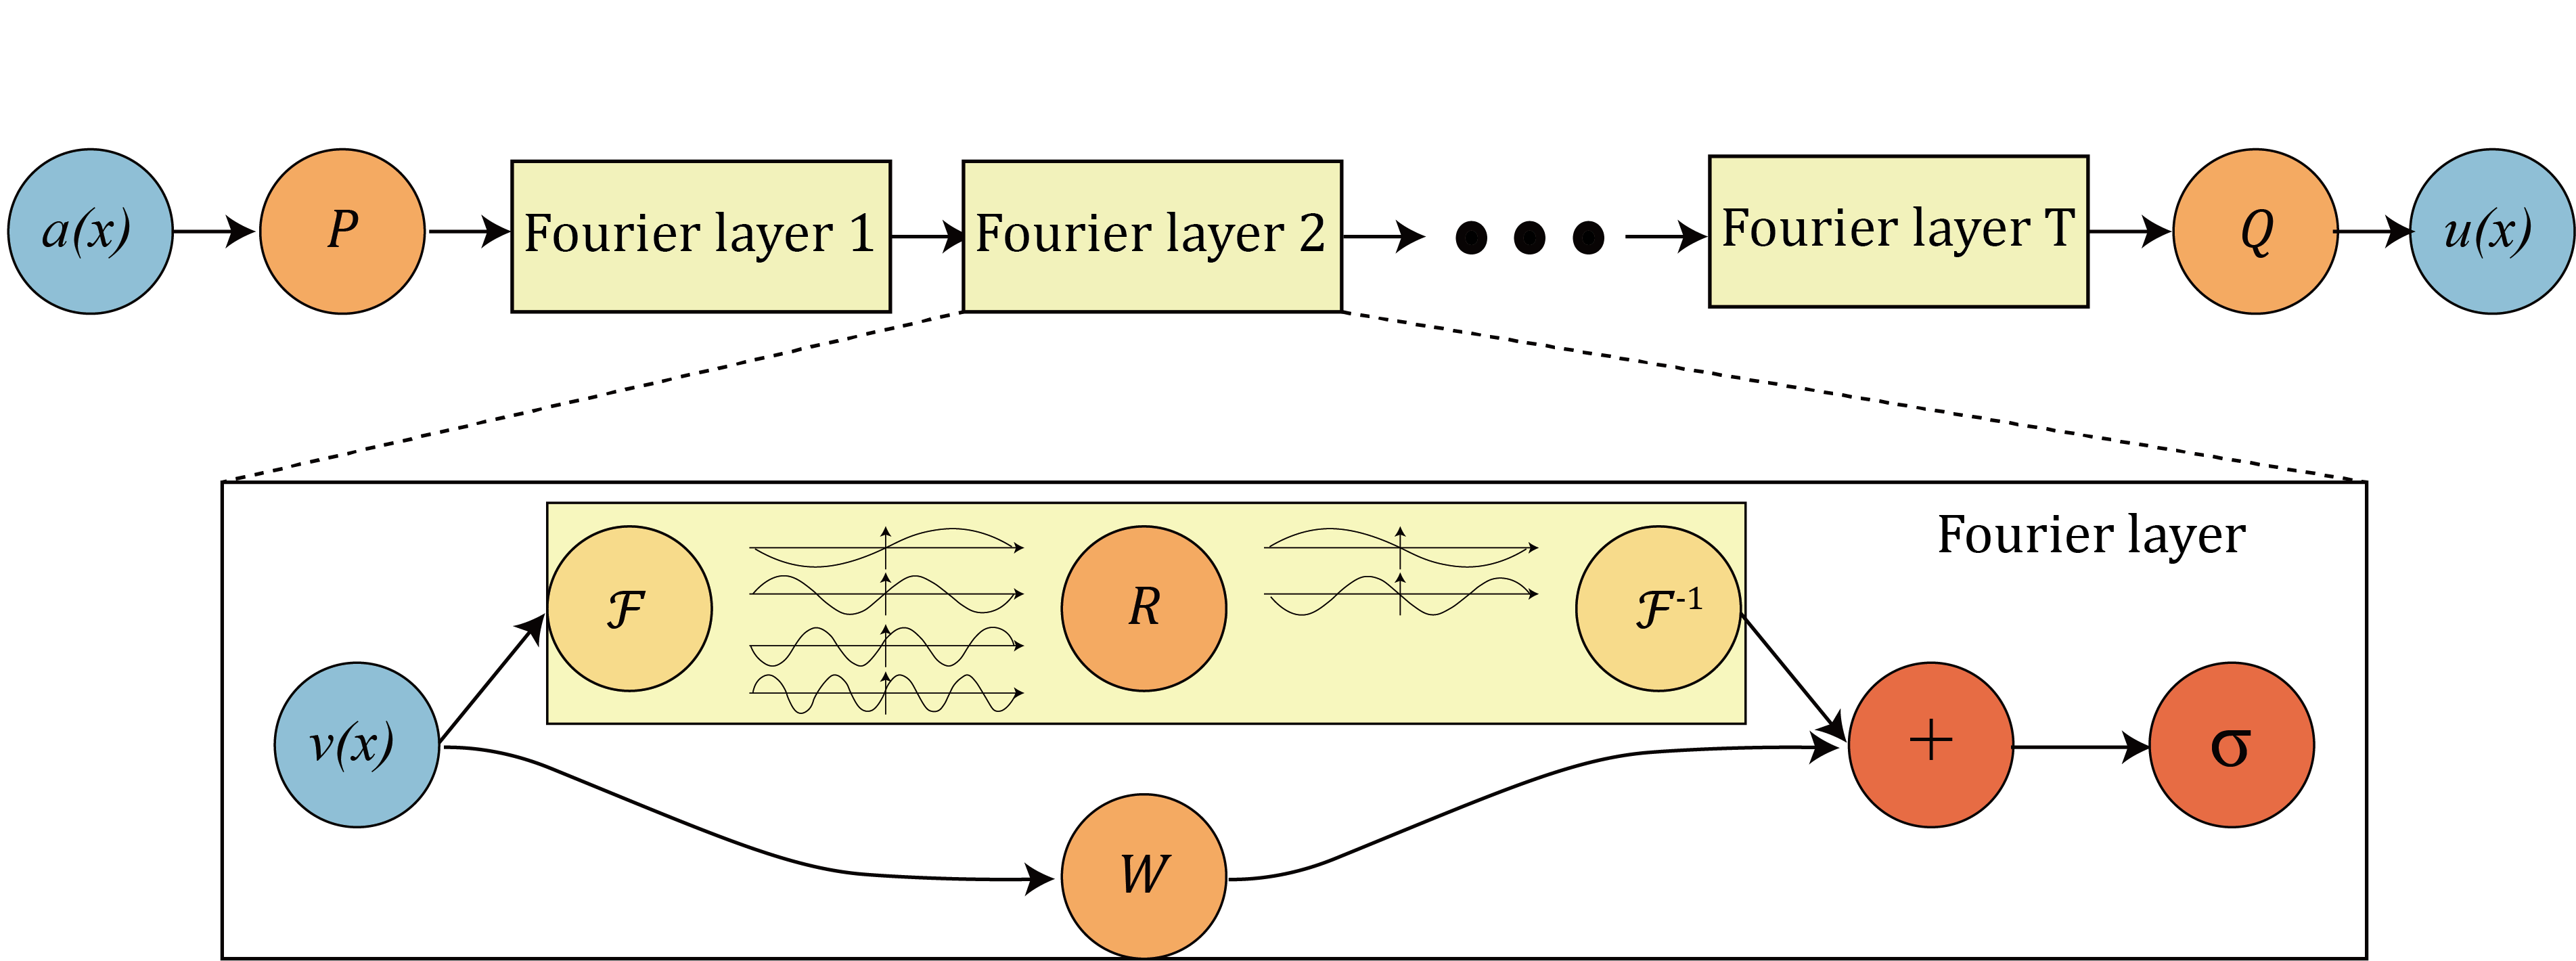
\includegraphics[width=0.6\linewidth]{figures/fourier_full_arch.png}
                        \caption{Schematic FNO architecture \cite{li2021}}
                        \label{fig:FNO}
                    \end{figure}
                    In common practice, the mean squared error (MSE) or $L_2$ loss is utilized for training. 
				 \end{block}

\begin{block}{What Has Worked? Simple and Complicated Linear Systems}
We tested a four-layer FNO on a 2-DOF undamped mass-spring system. 

\begin{figure}
         \centering
         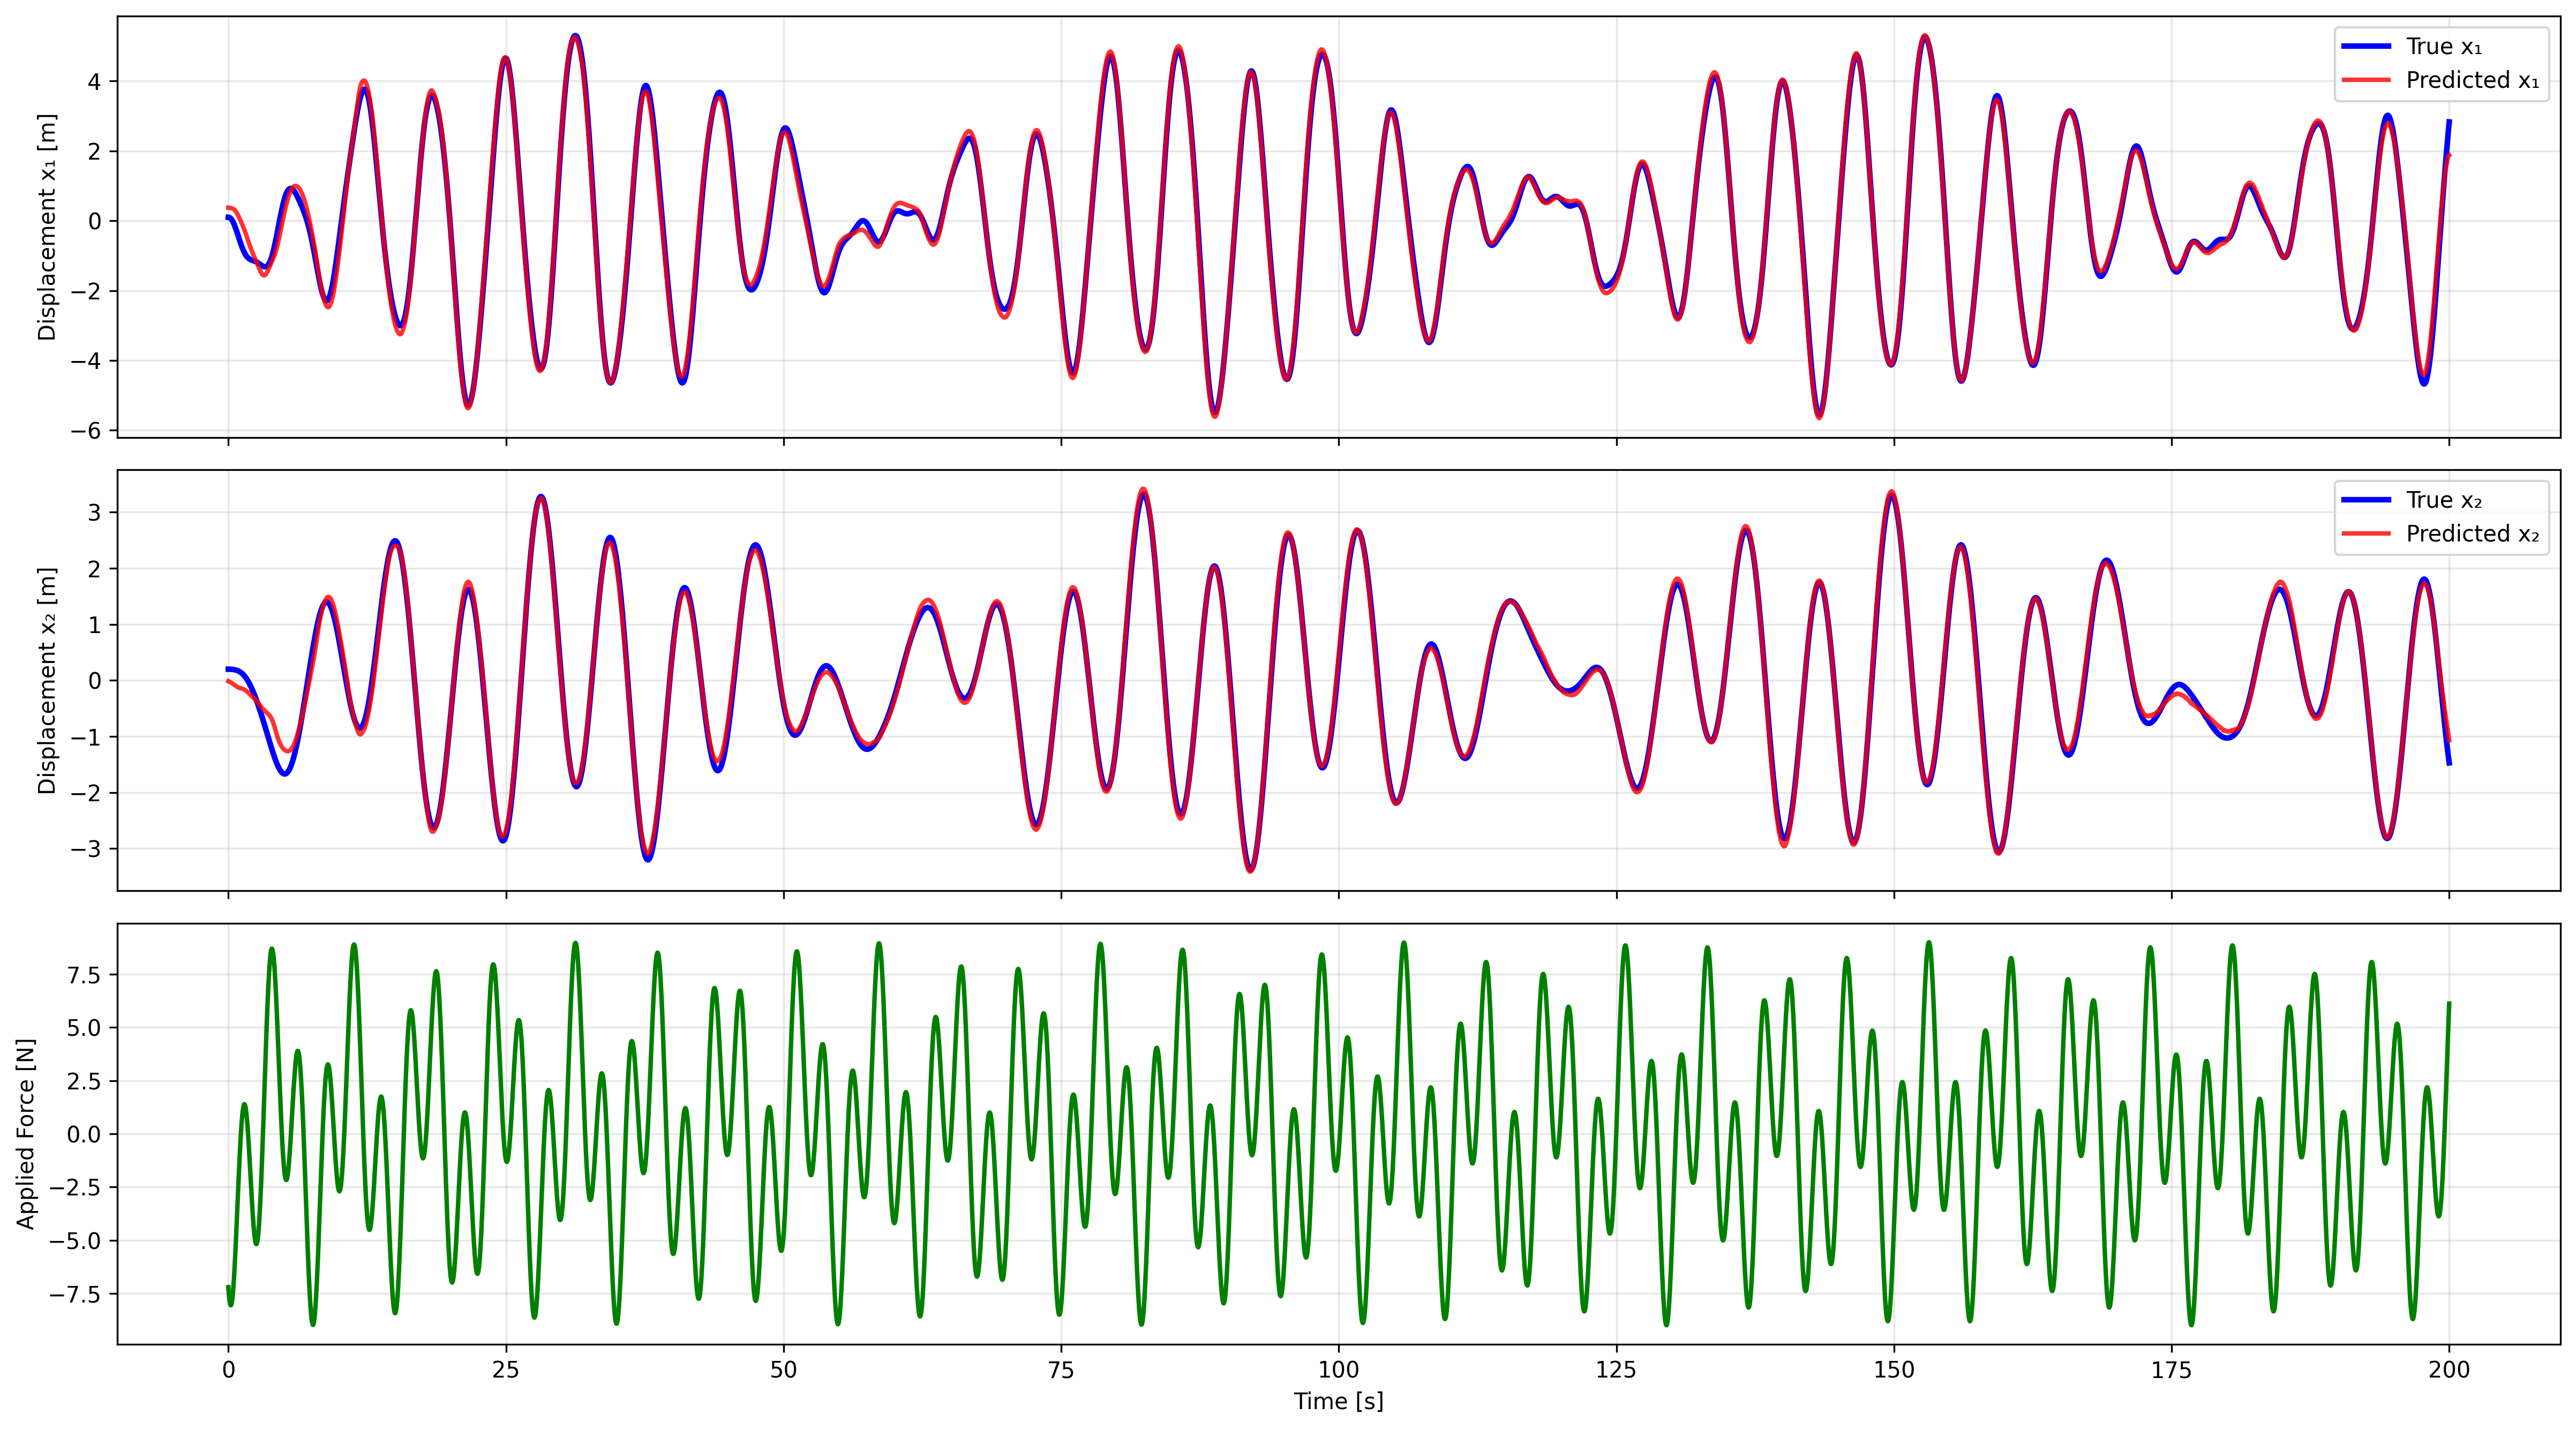
\includegraphics[width=0.6\linewidth]{figures/0066_0000_TFNO_2dof_linear_spectral.png}
         \caption{FNO test on linear 2-DOF mass-spring system}
         \label{fig:y equals x}
\end{figure}


We also utilized a similar architecture to build a virtual sensor for an offshore wind turbine model. For testing the FNO on an offshore wind turbine (OWT), we utilized publicly available OWT model simulation results \cite{Pedersen2024}. We propose the use of the FNO model as a virtual sensor for the moment time series measurements below the water line which are not accessible. 

\begin{figure}
     \centering
     \begin{subfigure}[t]{0.65\linewidth}
        \centering
    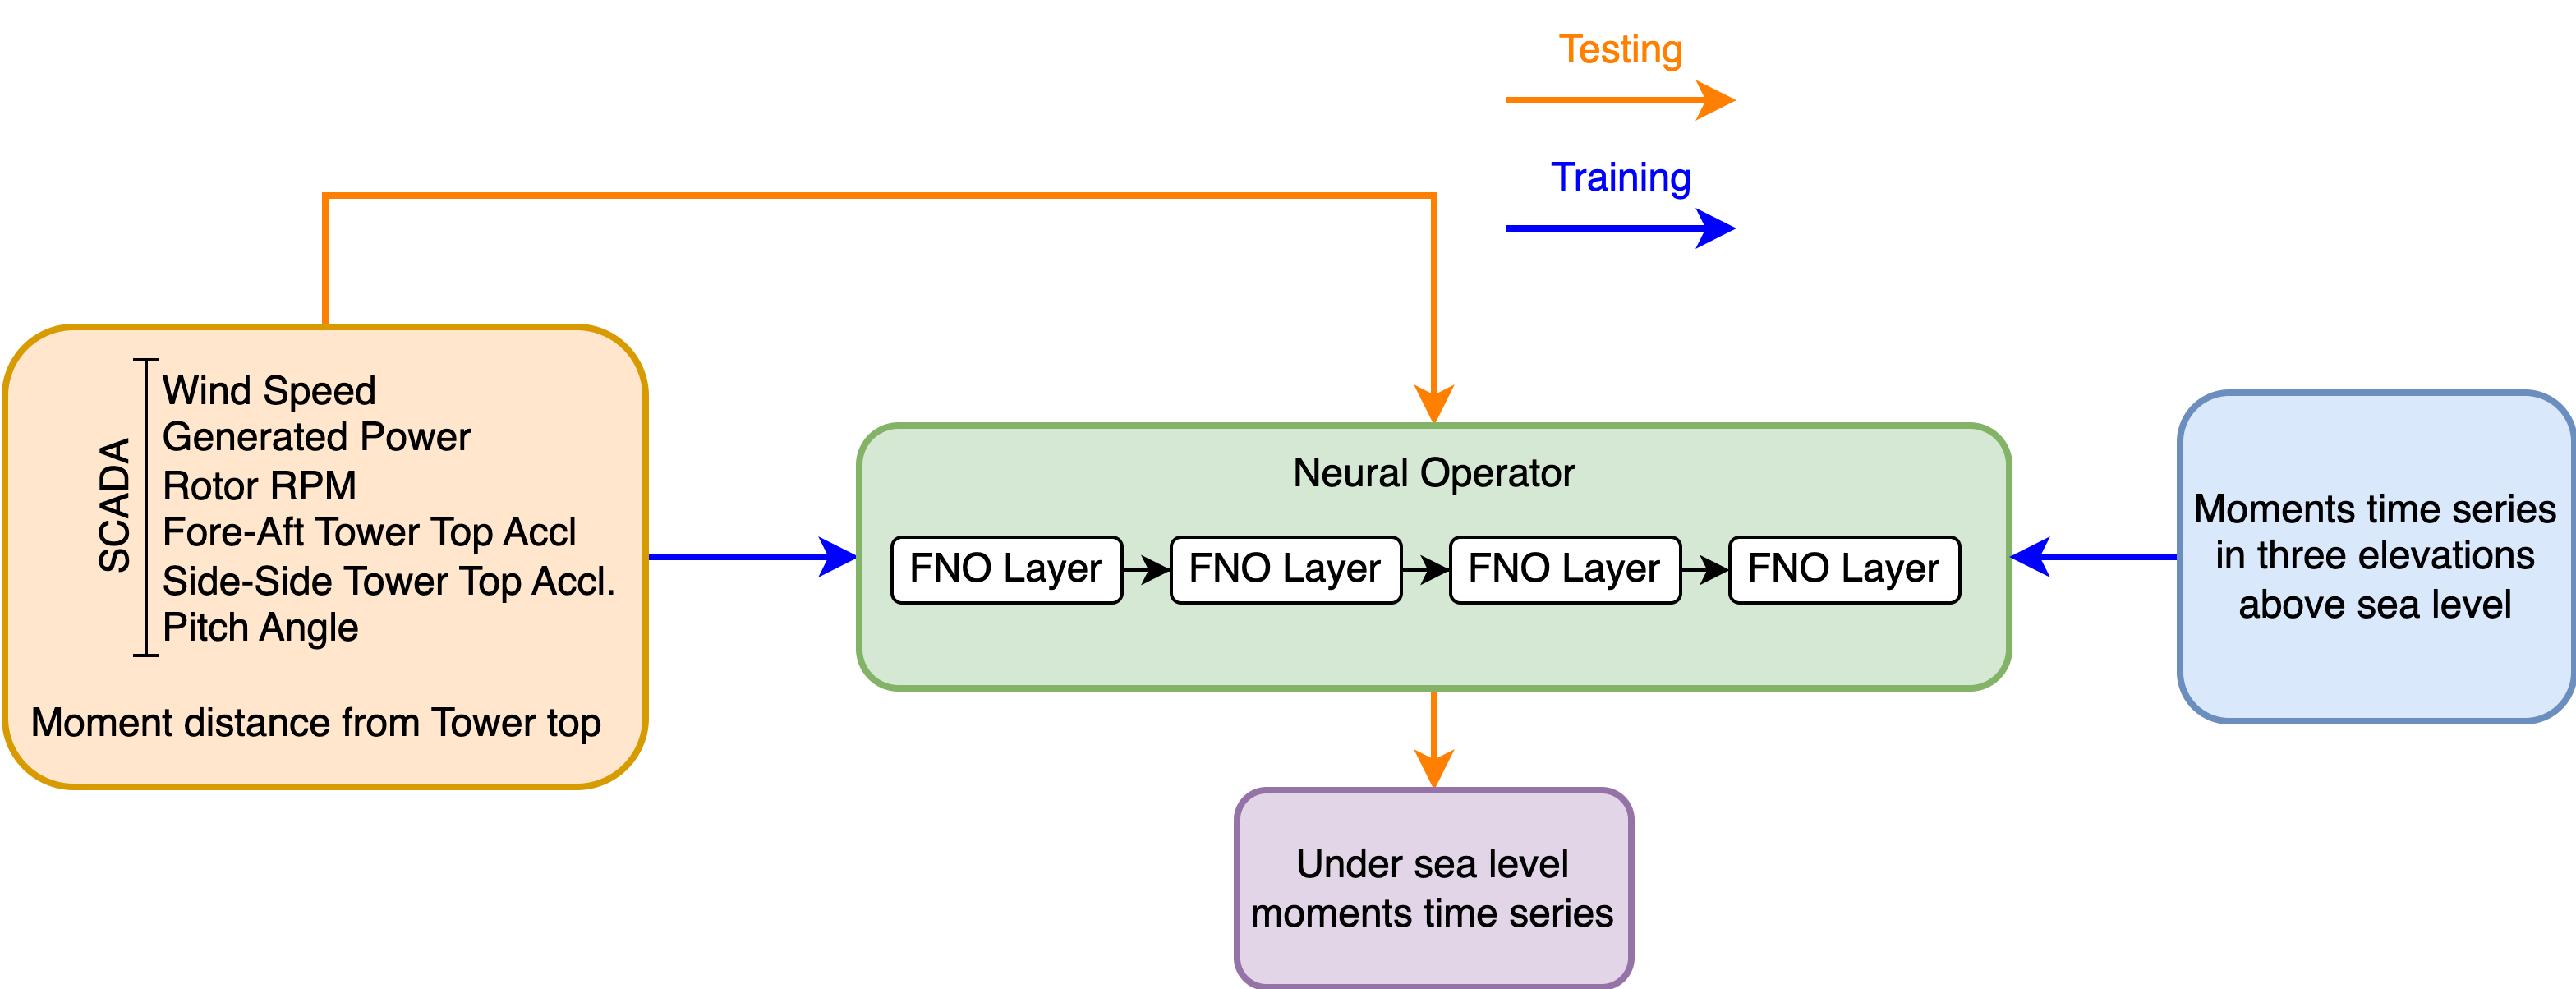
\includegraphics[width=1\linewidth]{figures/WESC2025_Abstract-Page-3.png}
    \caption{FNO as a virtual sensor for an Offshore Wind Turbine}
    %\label{fig:enter-label}
     \end{subfigure}
     \hfill
     \begin{subfigure}[t]{0.34\linewidth}
         \centering
         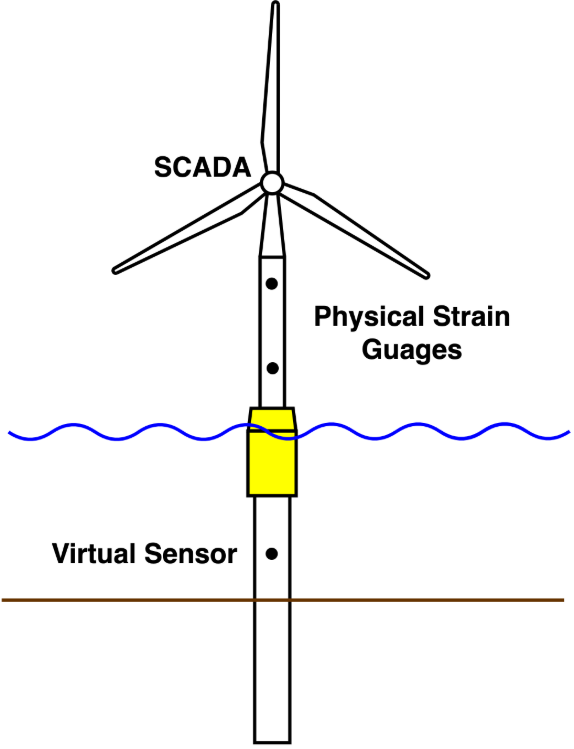
\includegraphics[width=0.8\linewidth]{figures/MassCEC.png}
         \caption{Offshore Wind Turbine virtual sensor}
         %\label{fig:three sin x}
     \end{subfigure}
\end{figure}



% \begin{figure}
%     \centering
%     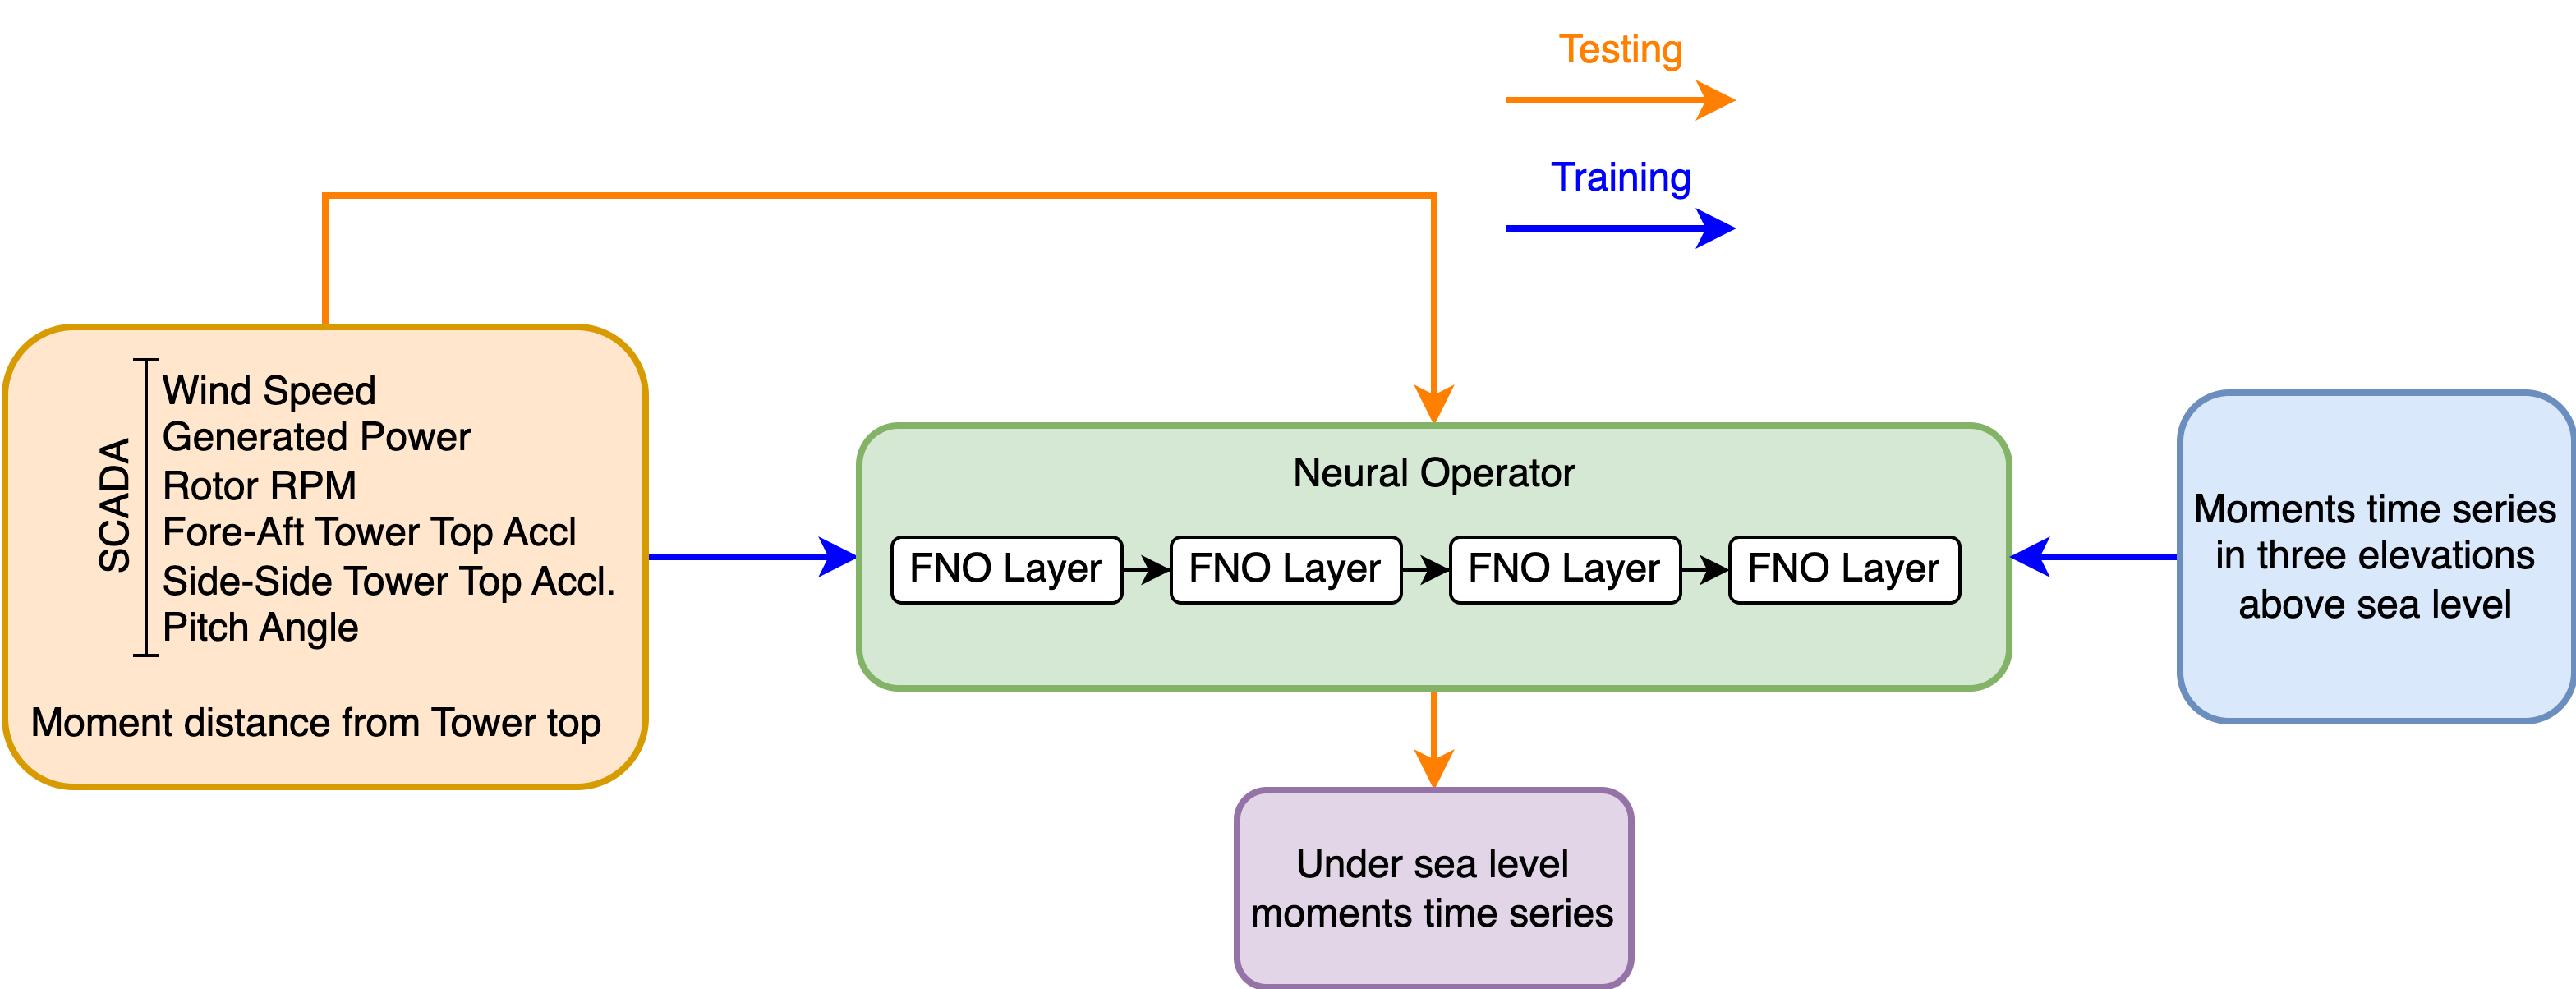
\includegraphics[width=0.75\linewidth]{figures/WESC2025_Abstract-Page-3.png}
%     \caption{FNO as a virtual sensor for an Offshore Wind Turbine}
%     %\label{fig:enter-label}
% \end{figure}

We show that the FNO can accurately predict the moment time series for the location along the foundation that it is not trained, indicating successful operator learning and generalization in function space.


% \begin{figure}
%     \centering
%     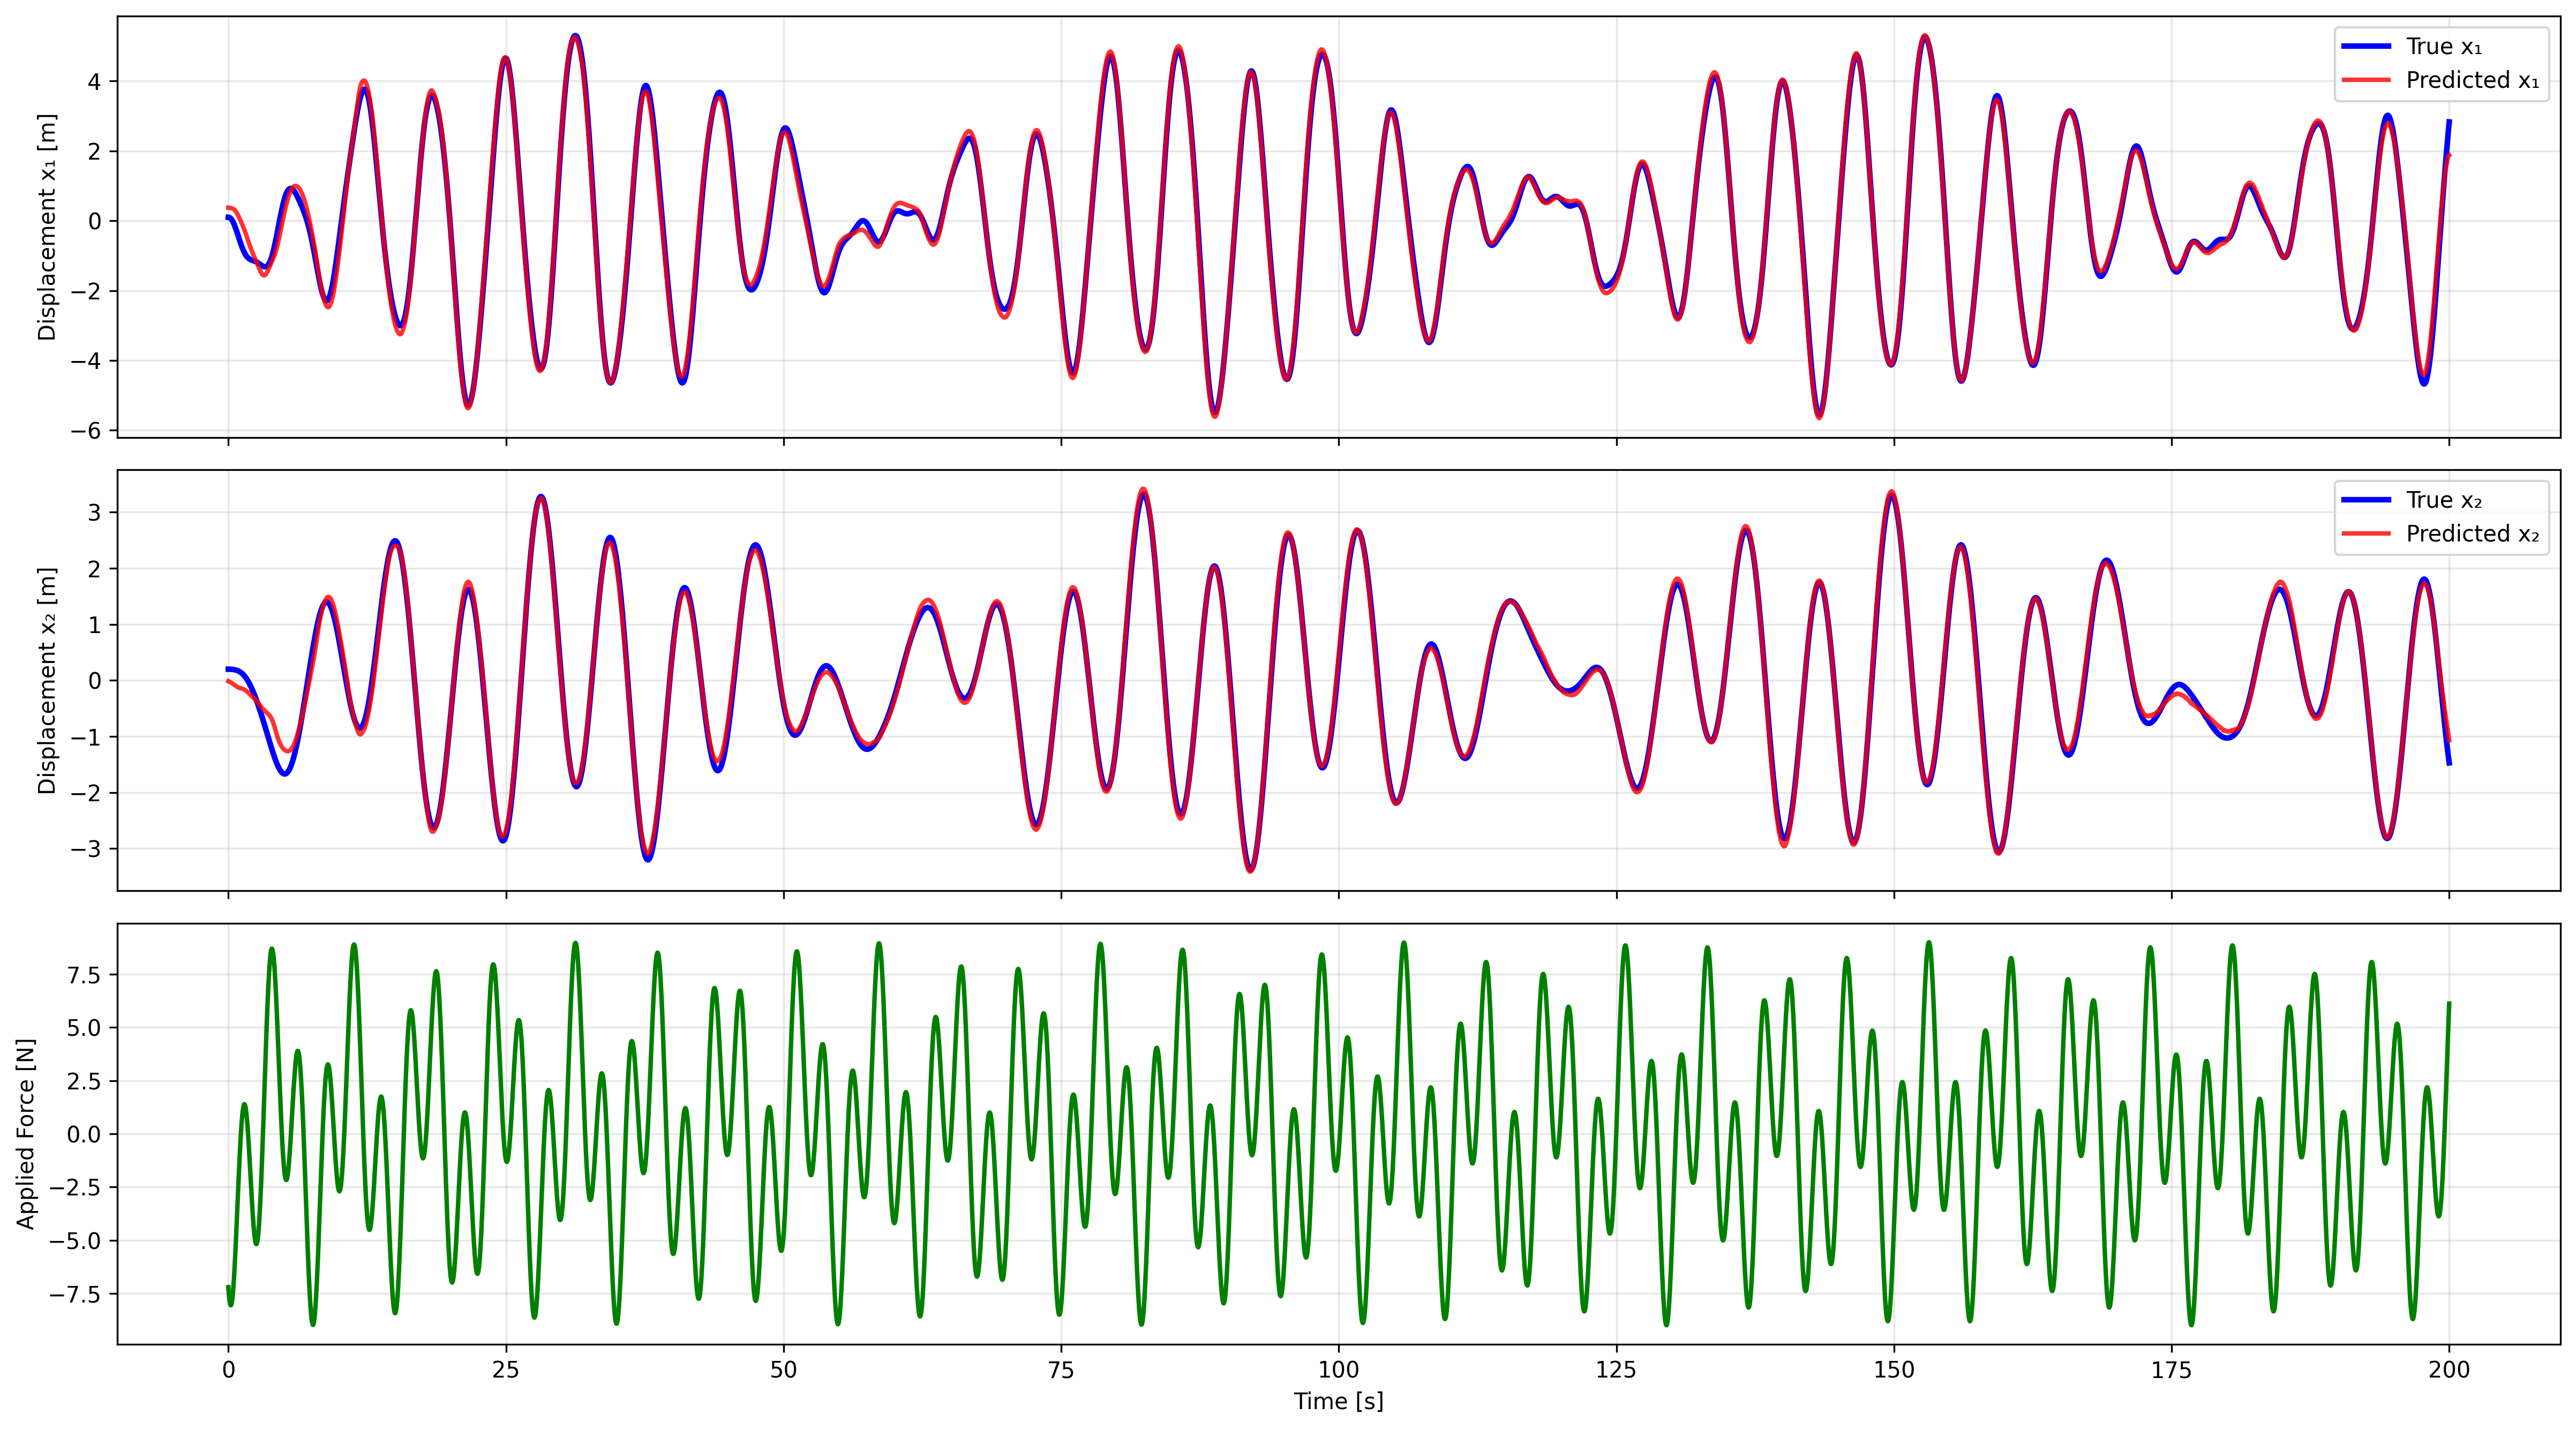
\includegraphics[width=0.5\linewidth]{figures/0066_0000_TFNO_2dof_linear_spectral.png}
%     \caption{2 DOF mass spring system test results}
%     %\label{fig:enter-label}

     \begin{figure}
         \centering
         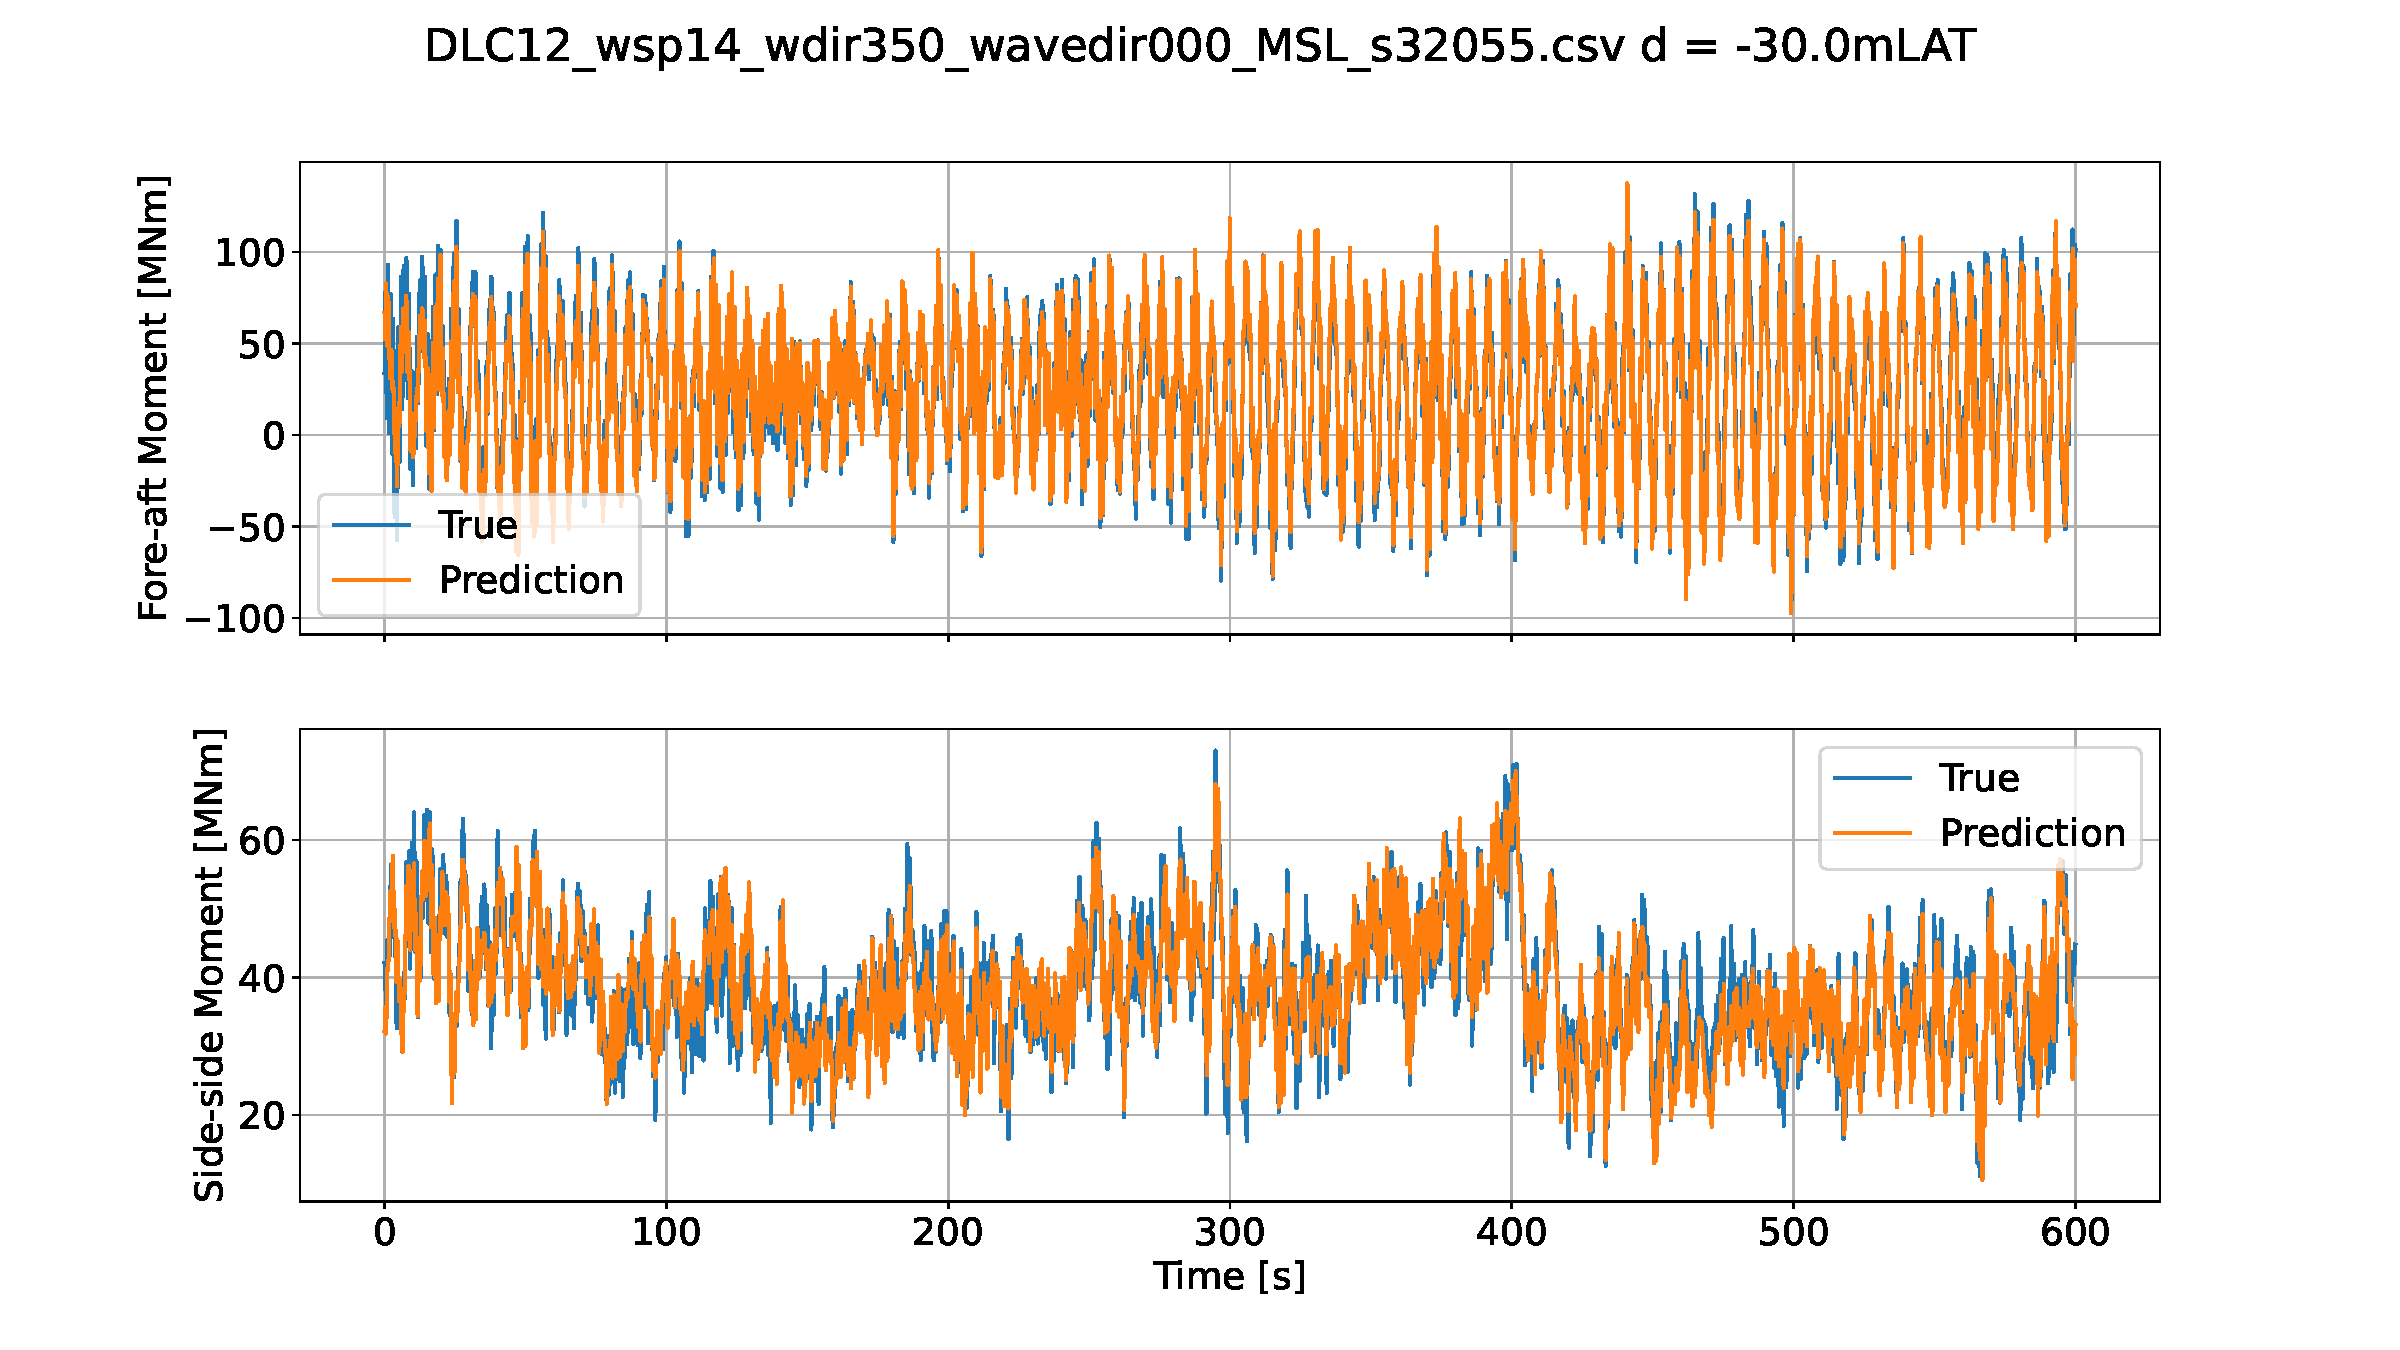
\includegraphics[trim={0 0 0 2cm},clip,width=0.6\linewidth]{figures/0000_DLC12_wsp14_wdir350_wavedir000_MSL_s32055.csv_0.0.pdf}
         \caption{FNO as a virtual sensor for an OWT simulation results}
         %\label{fig:three sin x}
     \end{figure}





% \begin{figure}
%     \centering
%     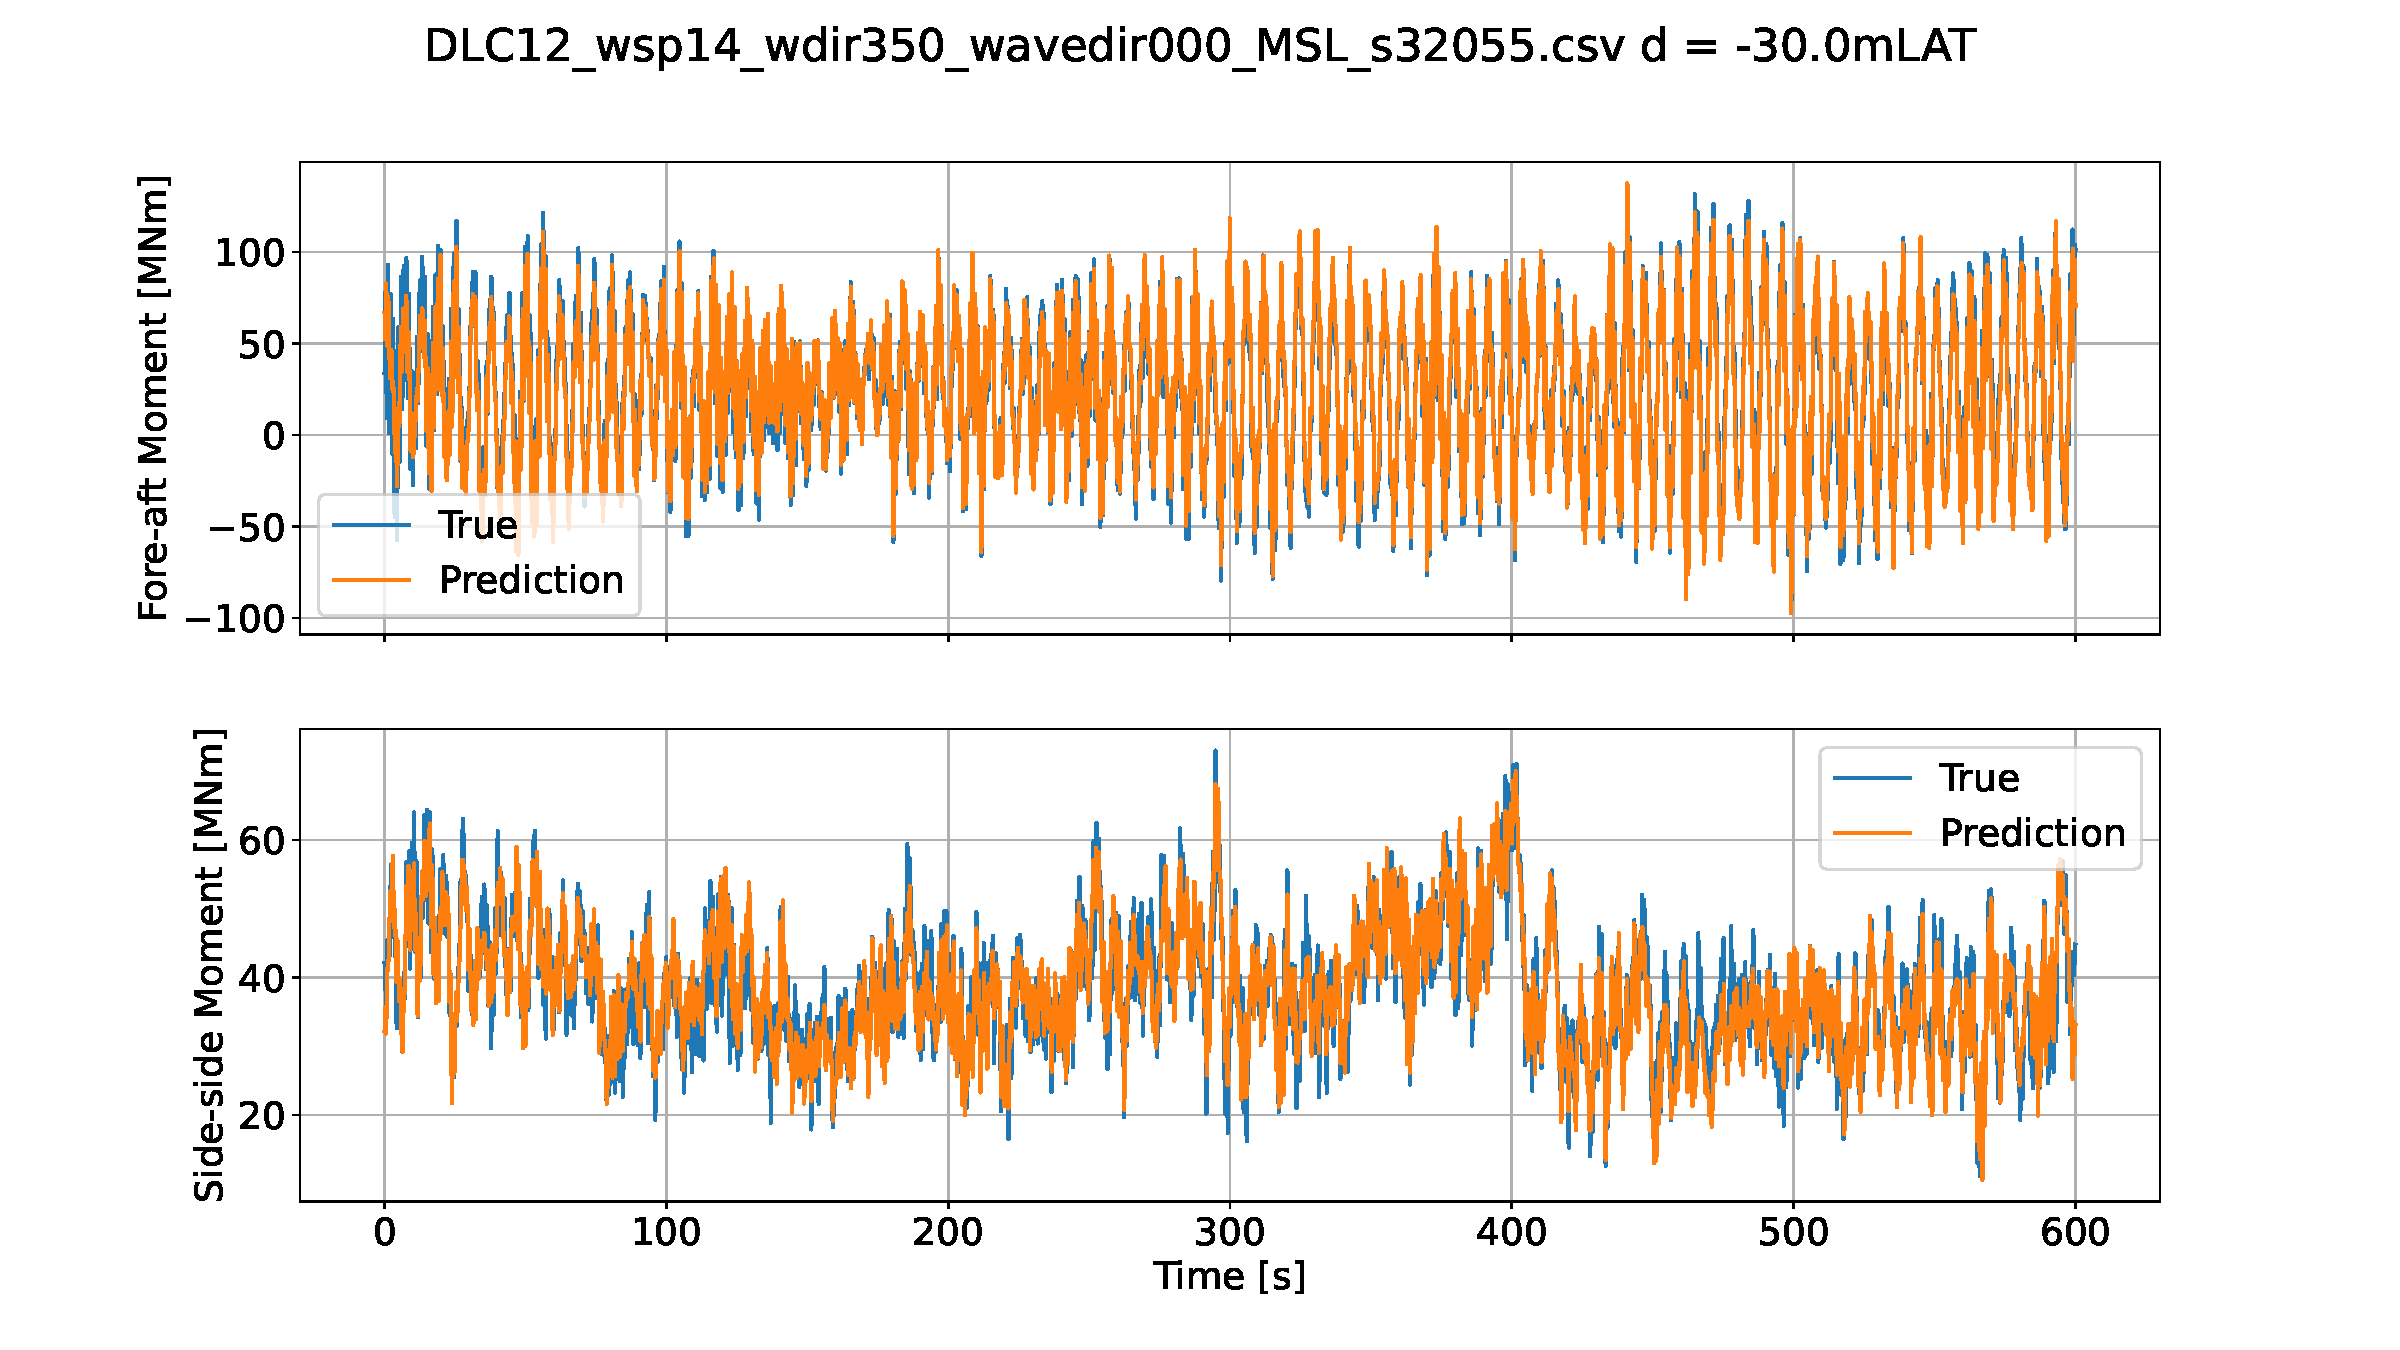
\includegraphics[width=0.5\linewidth]{figures/0000_DLC12_wsp14_wdir350_wavedir000_MSL_s32055.csv_0.0.pdf}
%     \caption{Moments time series prediction for IEA 15MW Offshore Wind Turbine, for an unseen location by FNO}
%     \label{fig:enter-label}
% \end{figure}
 \end{block}

% \begin{block}{Test Problem}
% \begin{table}[h!]
% \centering
% \renewcommand{\arraystretch}{2}
% \begin{tabular}{
% >{\raggedleft\arraybackslash}m{0.2\linewidth} 
% >{\centering\arraybackslash}m{0.4\linewidth} 
% >{\raggedleft\arraybackslash}m{0.2\linewidth}}

% 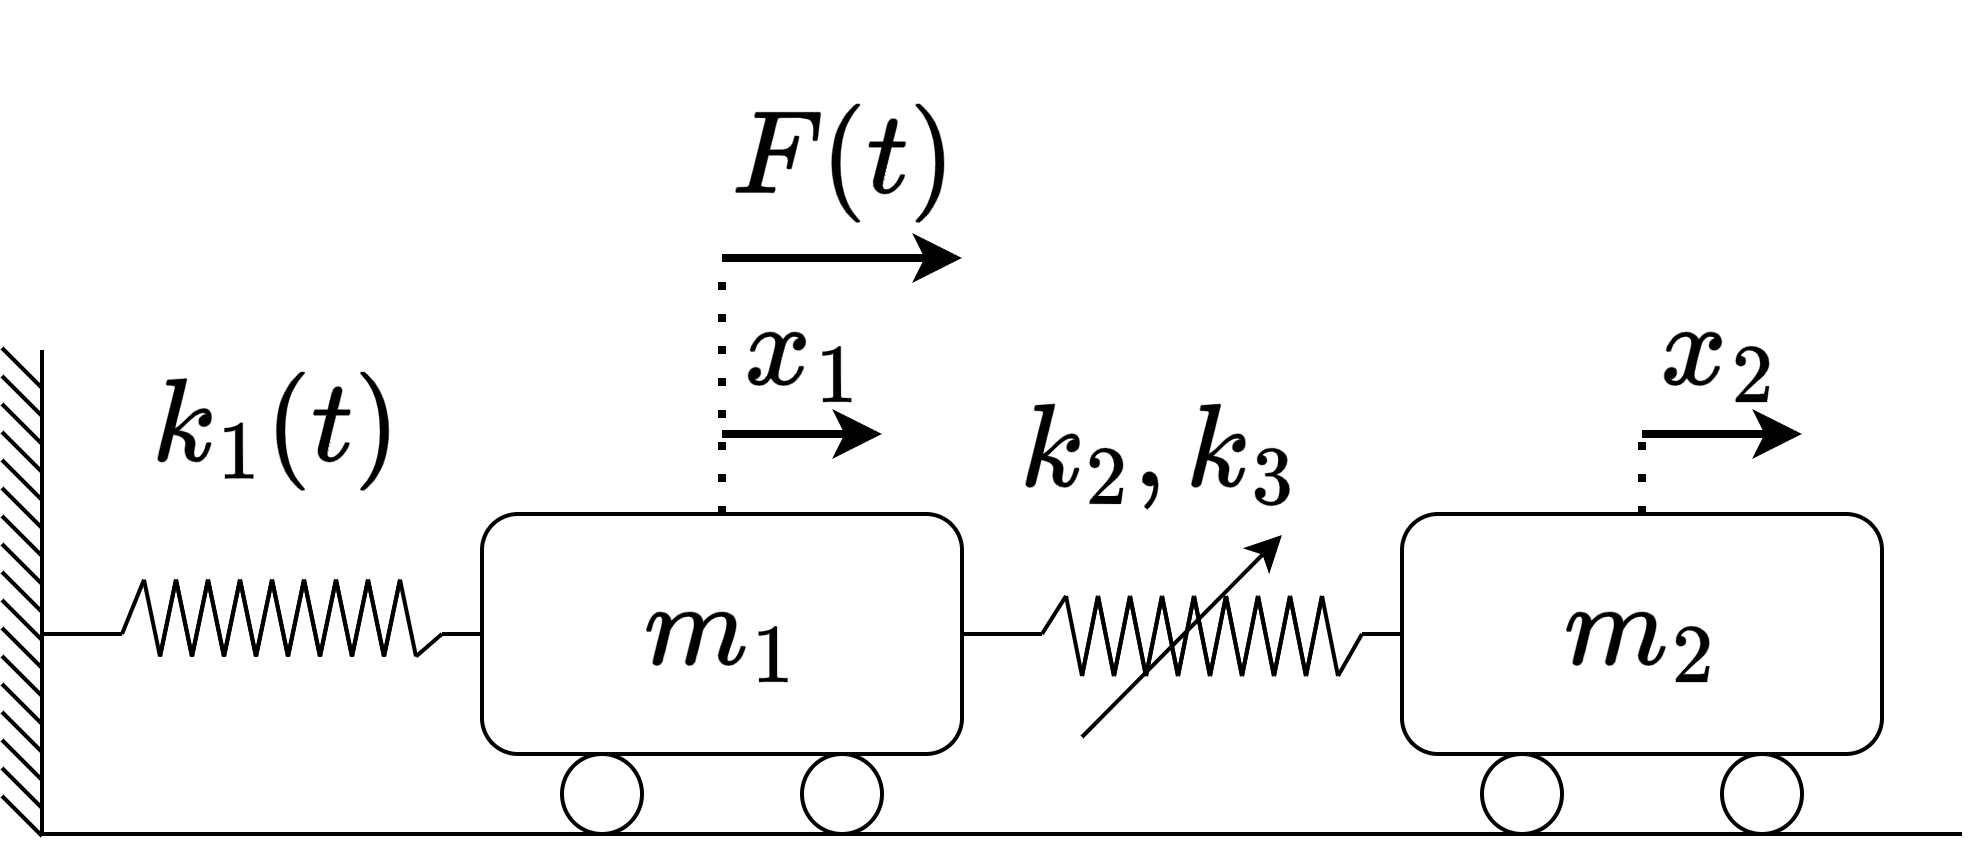
\includegraphics[width=1\linewidth]{figures/2DOF_MassSpring_k1_t.png} &

% \(\displaystyle
% \begin{aligned}
%     &m_{1}\ddot{x}_1 + k_1(t) x_1 + k_2(x_1 - x_2)+ k_3(x_1 - x_2)^3 = F(t) \\
%     &m_{2}\ddot{x}_2 + k_2(x_2 - x_1) + k_3(x_2 - x_1)^3 = 0\\
%     &k_{1}(t) = k_{0} + k_{initial}e^{-\alpha t}\\
%     &F(t) = A\sin(2\pi\omega_1t+\phi_1) + B\cos(2\pi\omega_2t+\phi_2)
% \end{aligned}
% \) &

% \(\displaystyle
% \begin{aligned}
%     x_1(0) &= 0.1,\:\dot{x}_1(0) = 0 \\
%     x_2(0) &= 0.2,\:\dot{x}_2(0) = 0
% \end{aligned}
% \)
% \\
% \end{tabular}
% %\caption{Figure and two sets of equations: dynamic model and initial conditions.}
% %\label{tab:fig_eq_table}
% \end{table}
% \vspace{0.5cm}
% Where  $m_1$ and $m_2$ are 5 and 10 kg, $k_{0}$ is 1 N/m, $k_{initial}$ is 3 N/m while $\alpha$ is 0.01. $k_2$ and $k_3$ are 3 N/m and 2 N/m$^3$. In the forcing function  $\omega_1$ and $\omega_2$ are 0.2 and 0.5 Hz. $A$ and $B$  are sampled from $\mathcal{U}(0,4)$ and $\mathcal{U}(0,5)$ utilizing Sobol's sampling method \cite{sobolDistributionPointsCube1967}, while $\phi_1$ and $\phi_2$  are sampled from $\mathcal{U}(0,2\pi)$. We build the dataset by taking $2^{12}$ samples from theses random variables and then generating the force time series. Afterwards, we solve the 2DOF system based on those force time series for the displacement of $m_1$ and $m_2$. The equation of motion was solved utilizing \texttt{scipy} Runge-Kutta-Fehlberg Method (RKF45).
% \end{block}


%\end{block}


            
 }
\end{minipage}
\end{beamercolorbox}
		

%----------------------------------------------------------Middle Column ---------------------------------------------------------------

\column{.5\textwidth}
\begin{beamercolorbox}[center,wd=\textwidth]{postercolumn}
\begin{minipage}[T]{.95\linewidth}  % tweaks the width, makes a new \textwidth
\parbox[t][\columnheight]{\textwidth}{ % must be some better way to set the the height, width and textwidth simultaneously
% Since all columns are the same length, it is all nice and tidy.  You have to get the height empirical

% \begin{block}{What hasn't worked?}
%     We tested out of the box FNO with a non-linear cubic stiffening 2 DOF mass spring system. The goal was seeing if the FNO can predict the displacement time series of two mass when it gets the force time series as the input. The out of the box FNO with MSE loss did not function properly in our test. One solution is increasing the size of the datasets. We tested this on $2^{11}$,$2^{12}$,$2^{13}$ and $2^{14}$ dataset sizes. The results show no significant improvement in the results.
    
% \begin{figure}
%      \centering
%      \begin{subfigure}[b]{0.24\linewidth}
%          \centering
%          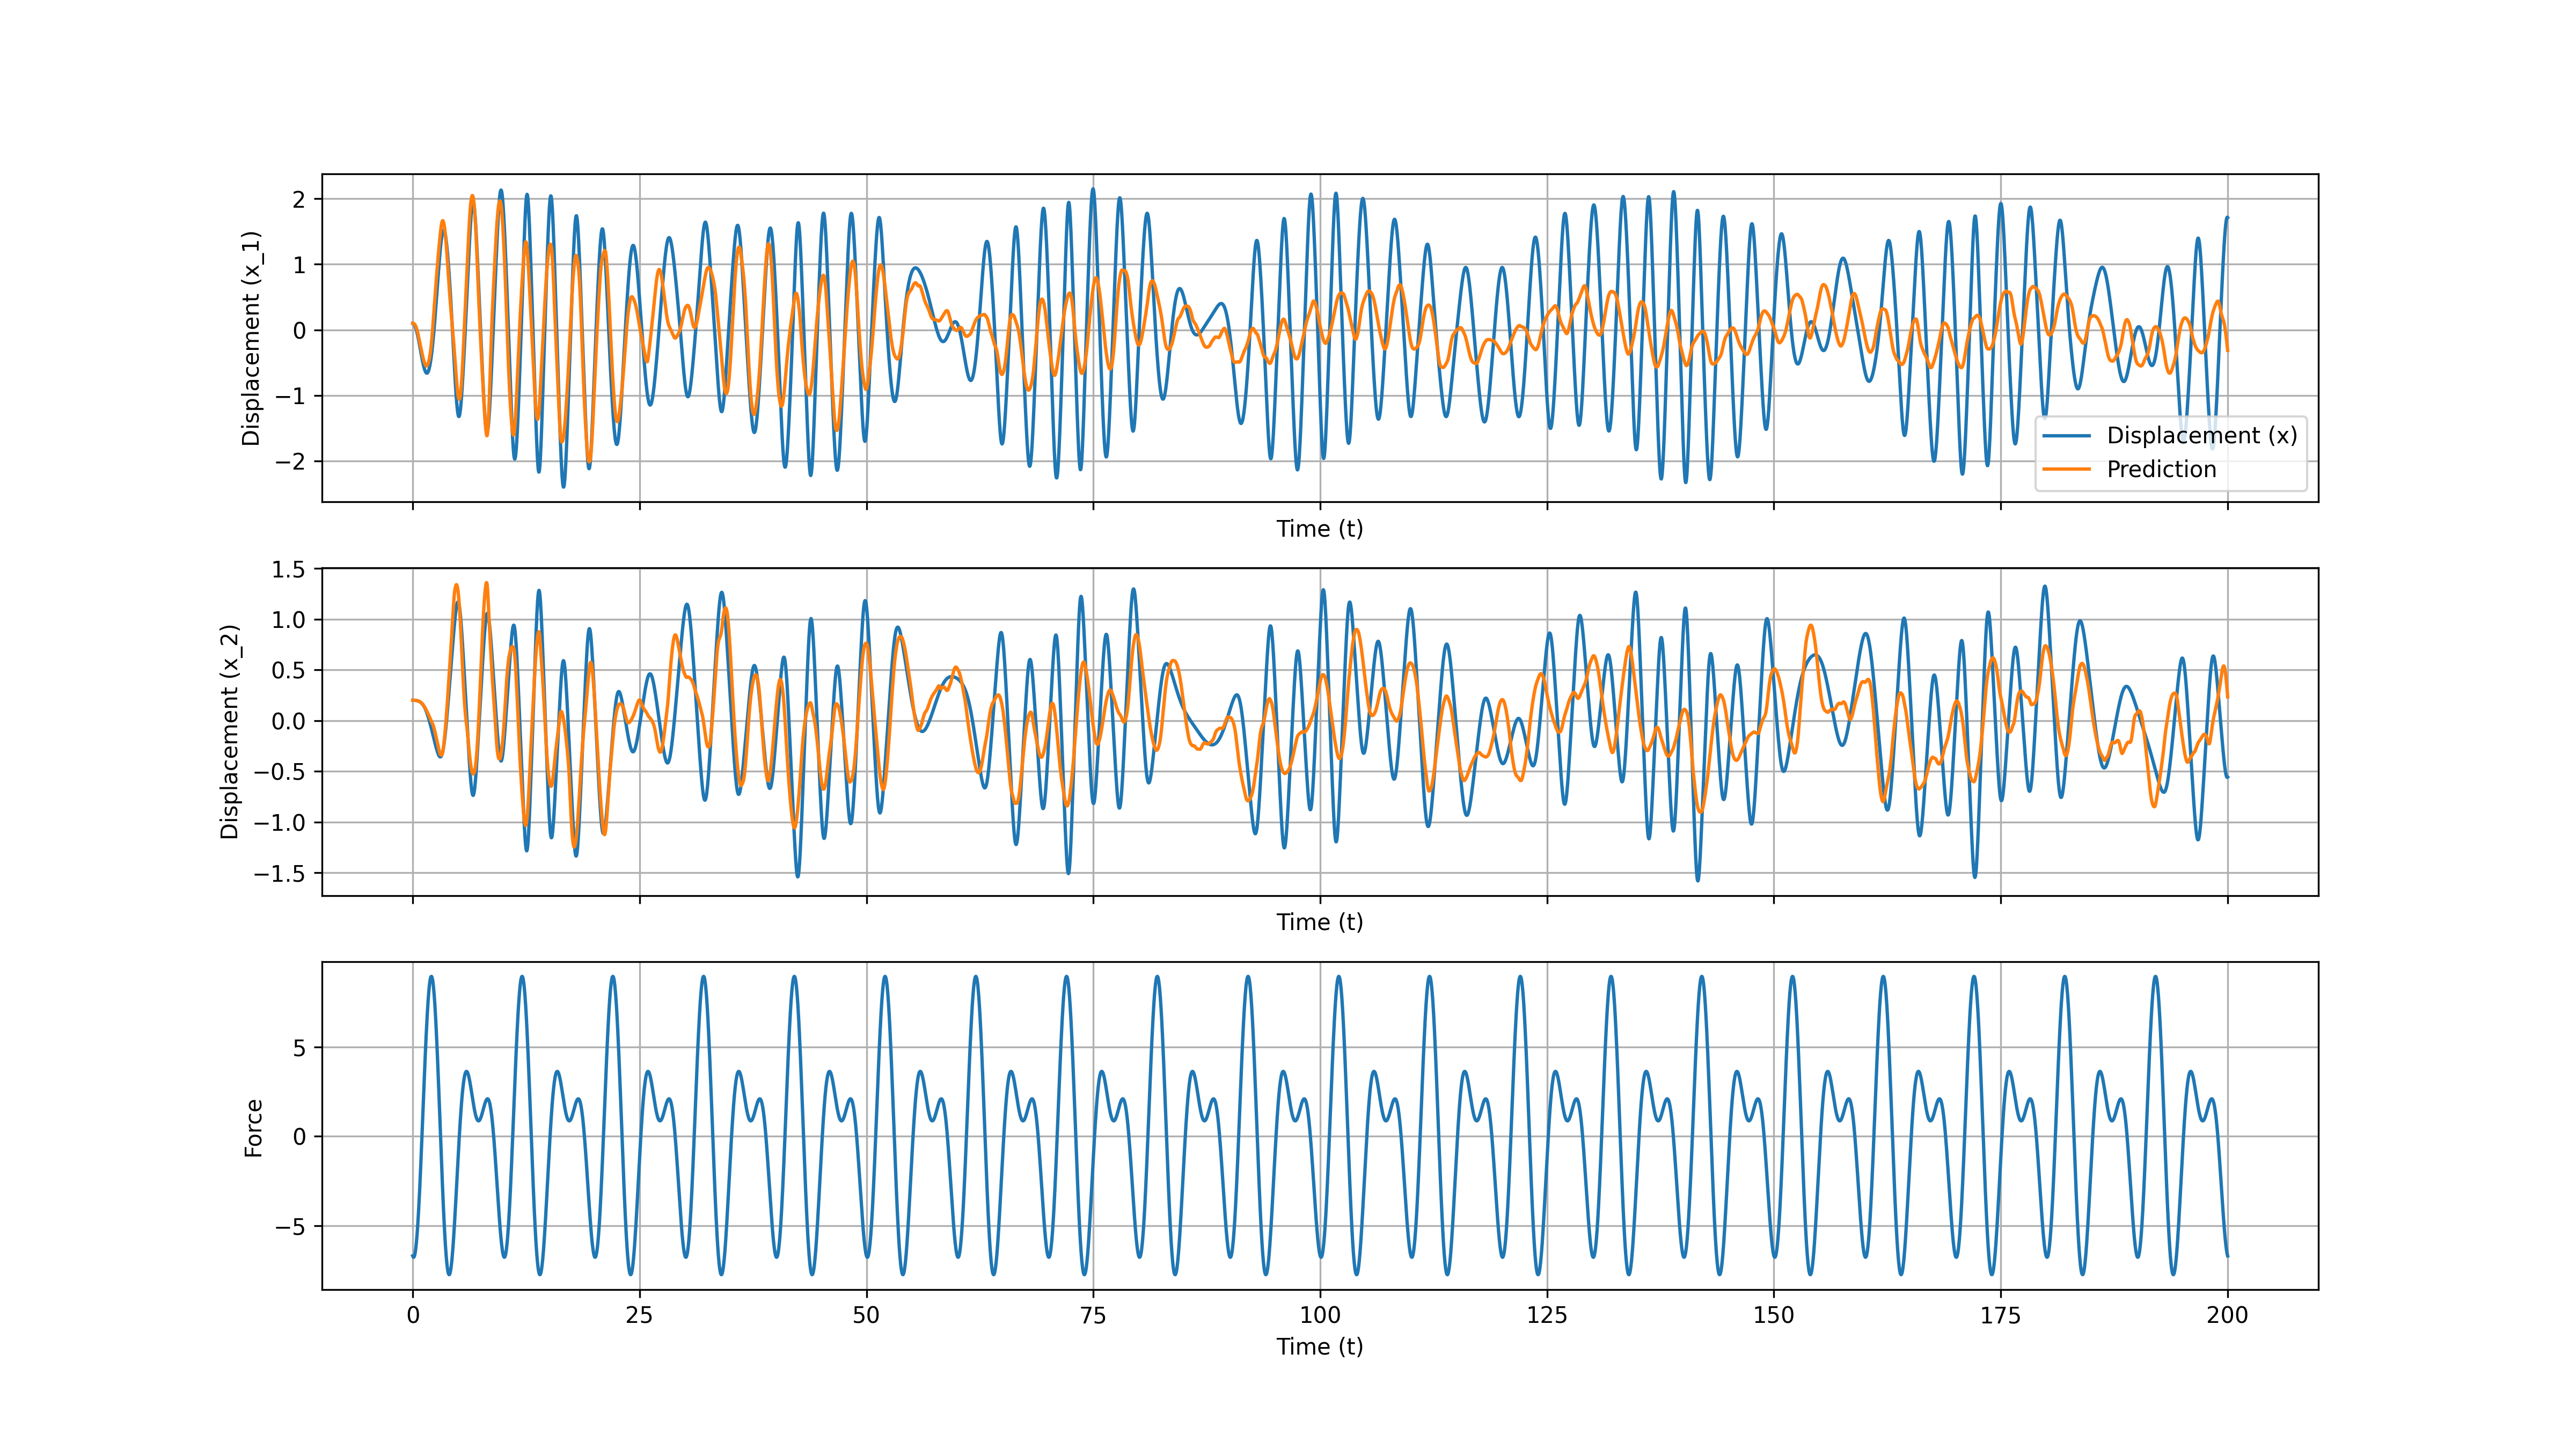
\includegraphics[width=\linewidth]{figures/2048_sobol_2dof_nlinear_tfno.png}
%          \caption{$2^{11}$ dataset testing result}
%          \label{fig:y equals x}
%      \end{subfigure}
%      \hfill
%      \begin{subfigure}[b]{0.24\linewidth}
%          \centering
%          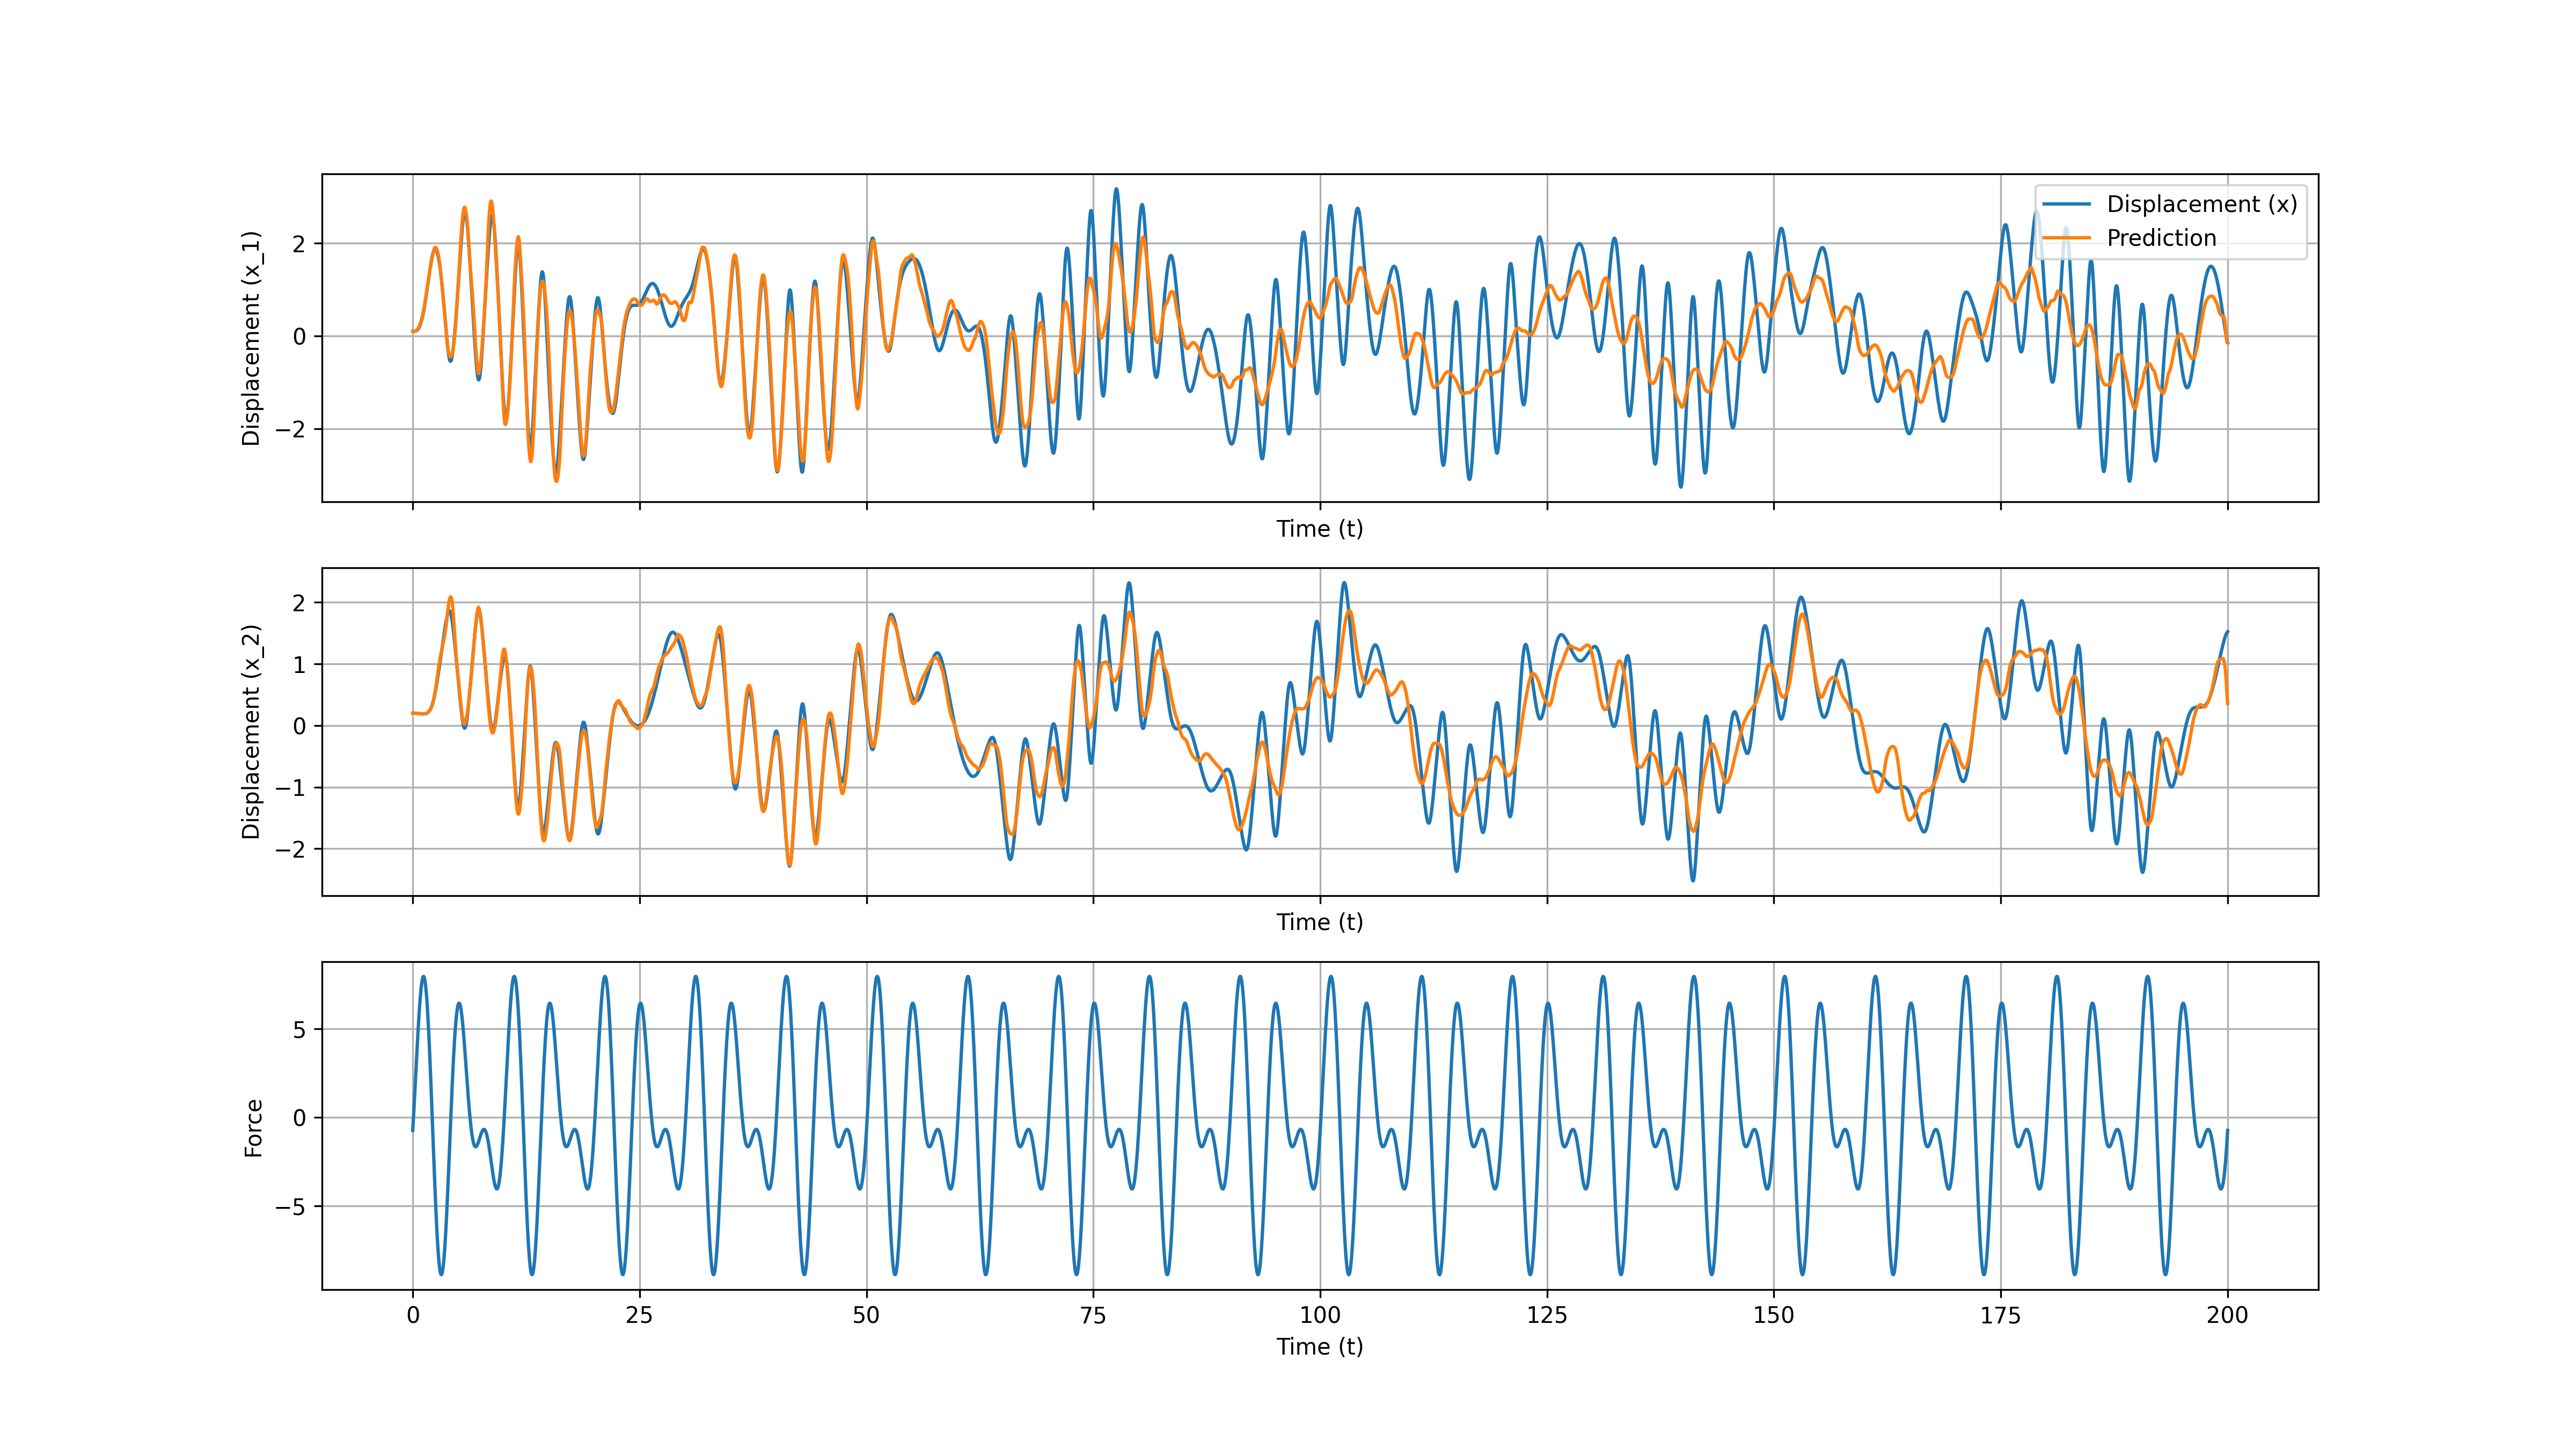
\includegraphics[width=\linewidth]{figures/4096_sobol_2dof_nlinear_tfno.png}
%          \caption{$2^{12}$ dataset testing result}
%          \label{fig:three sin x}
%      \end{subfigure}
%      \hfill
%      \begin{subfigure}[b]{0.24\linewidth}
%          \centering
%          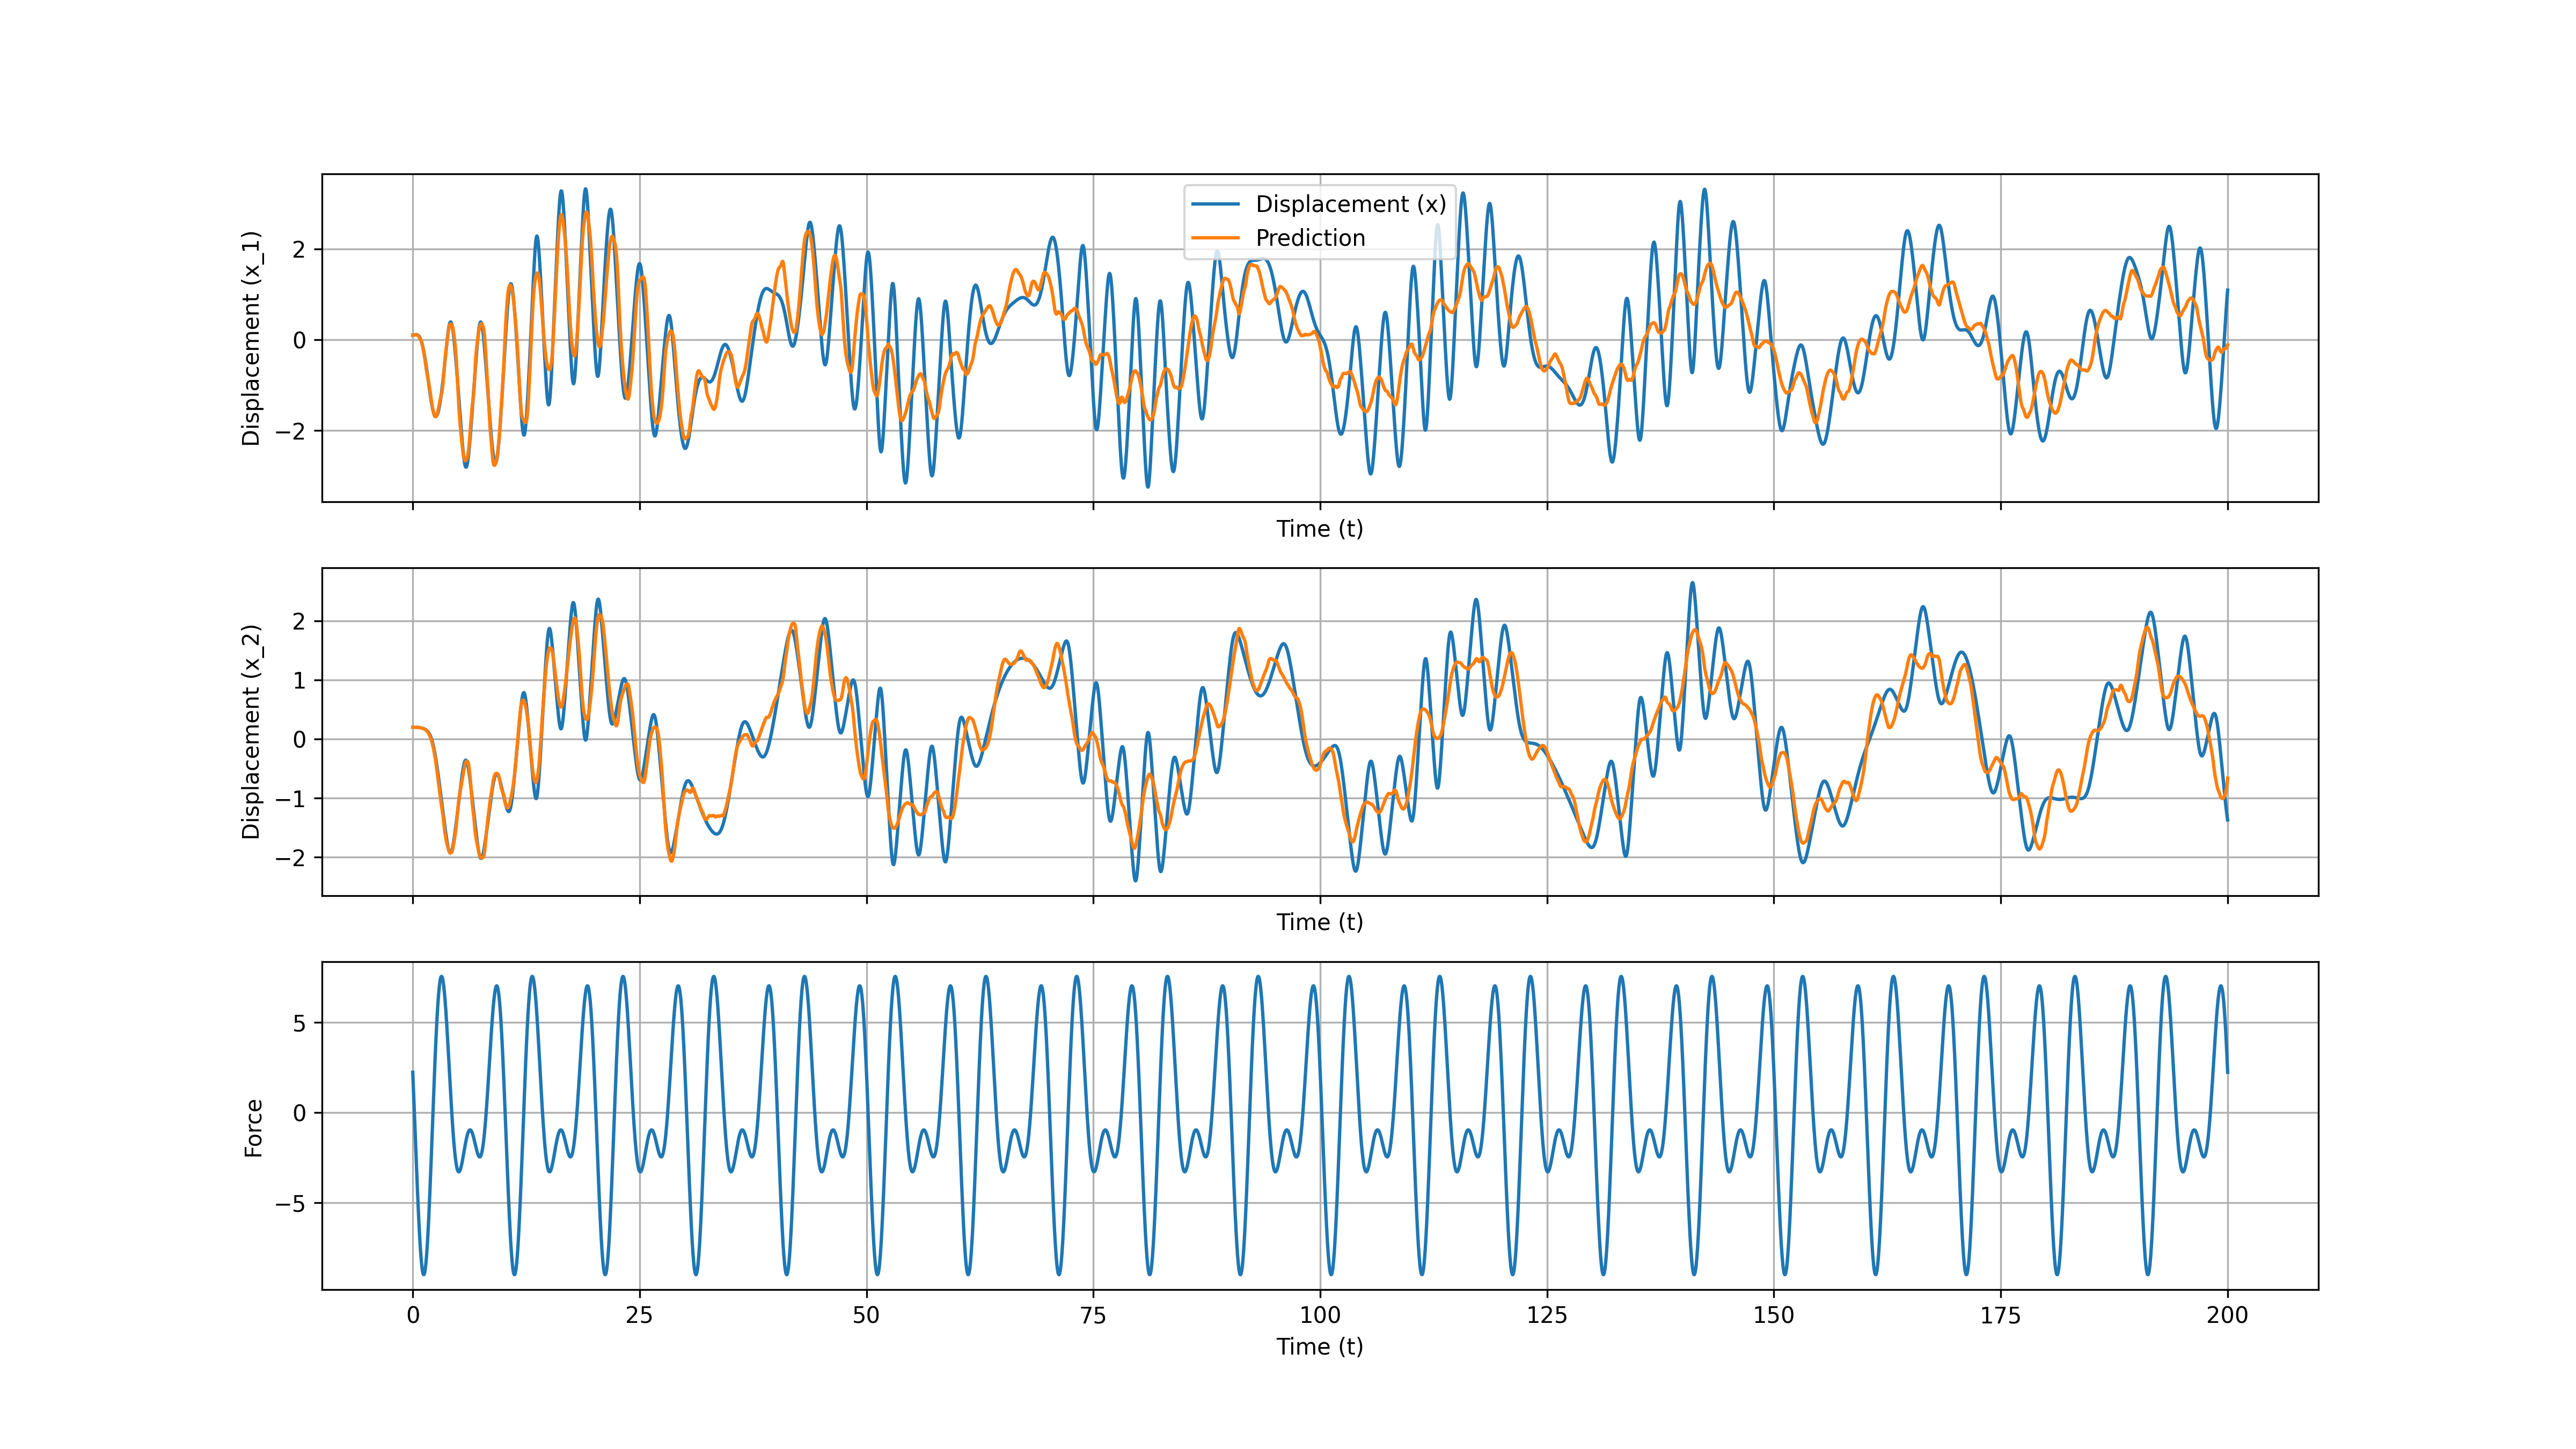
\includegraphics[width=\linewidth]{figures/8192_sobol_2dof_nlinear_tfno.png}
%          \caption{$2^{13}$ dataset testing result}
%          \label{fig:five over x}
%      \end{subfigure}
%      \hfill
%      \begin{subfigure}[b]{0.24\linewidth}
%          \centering
%          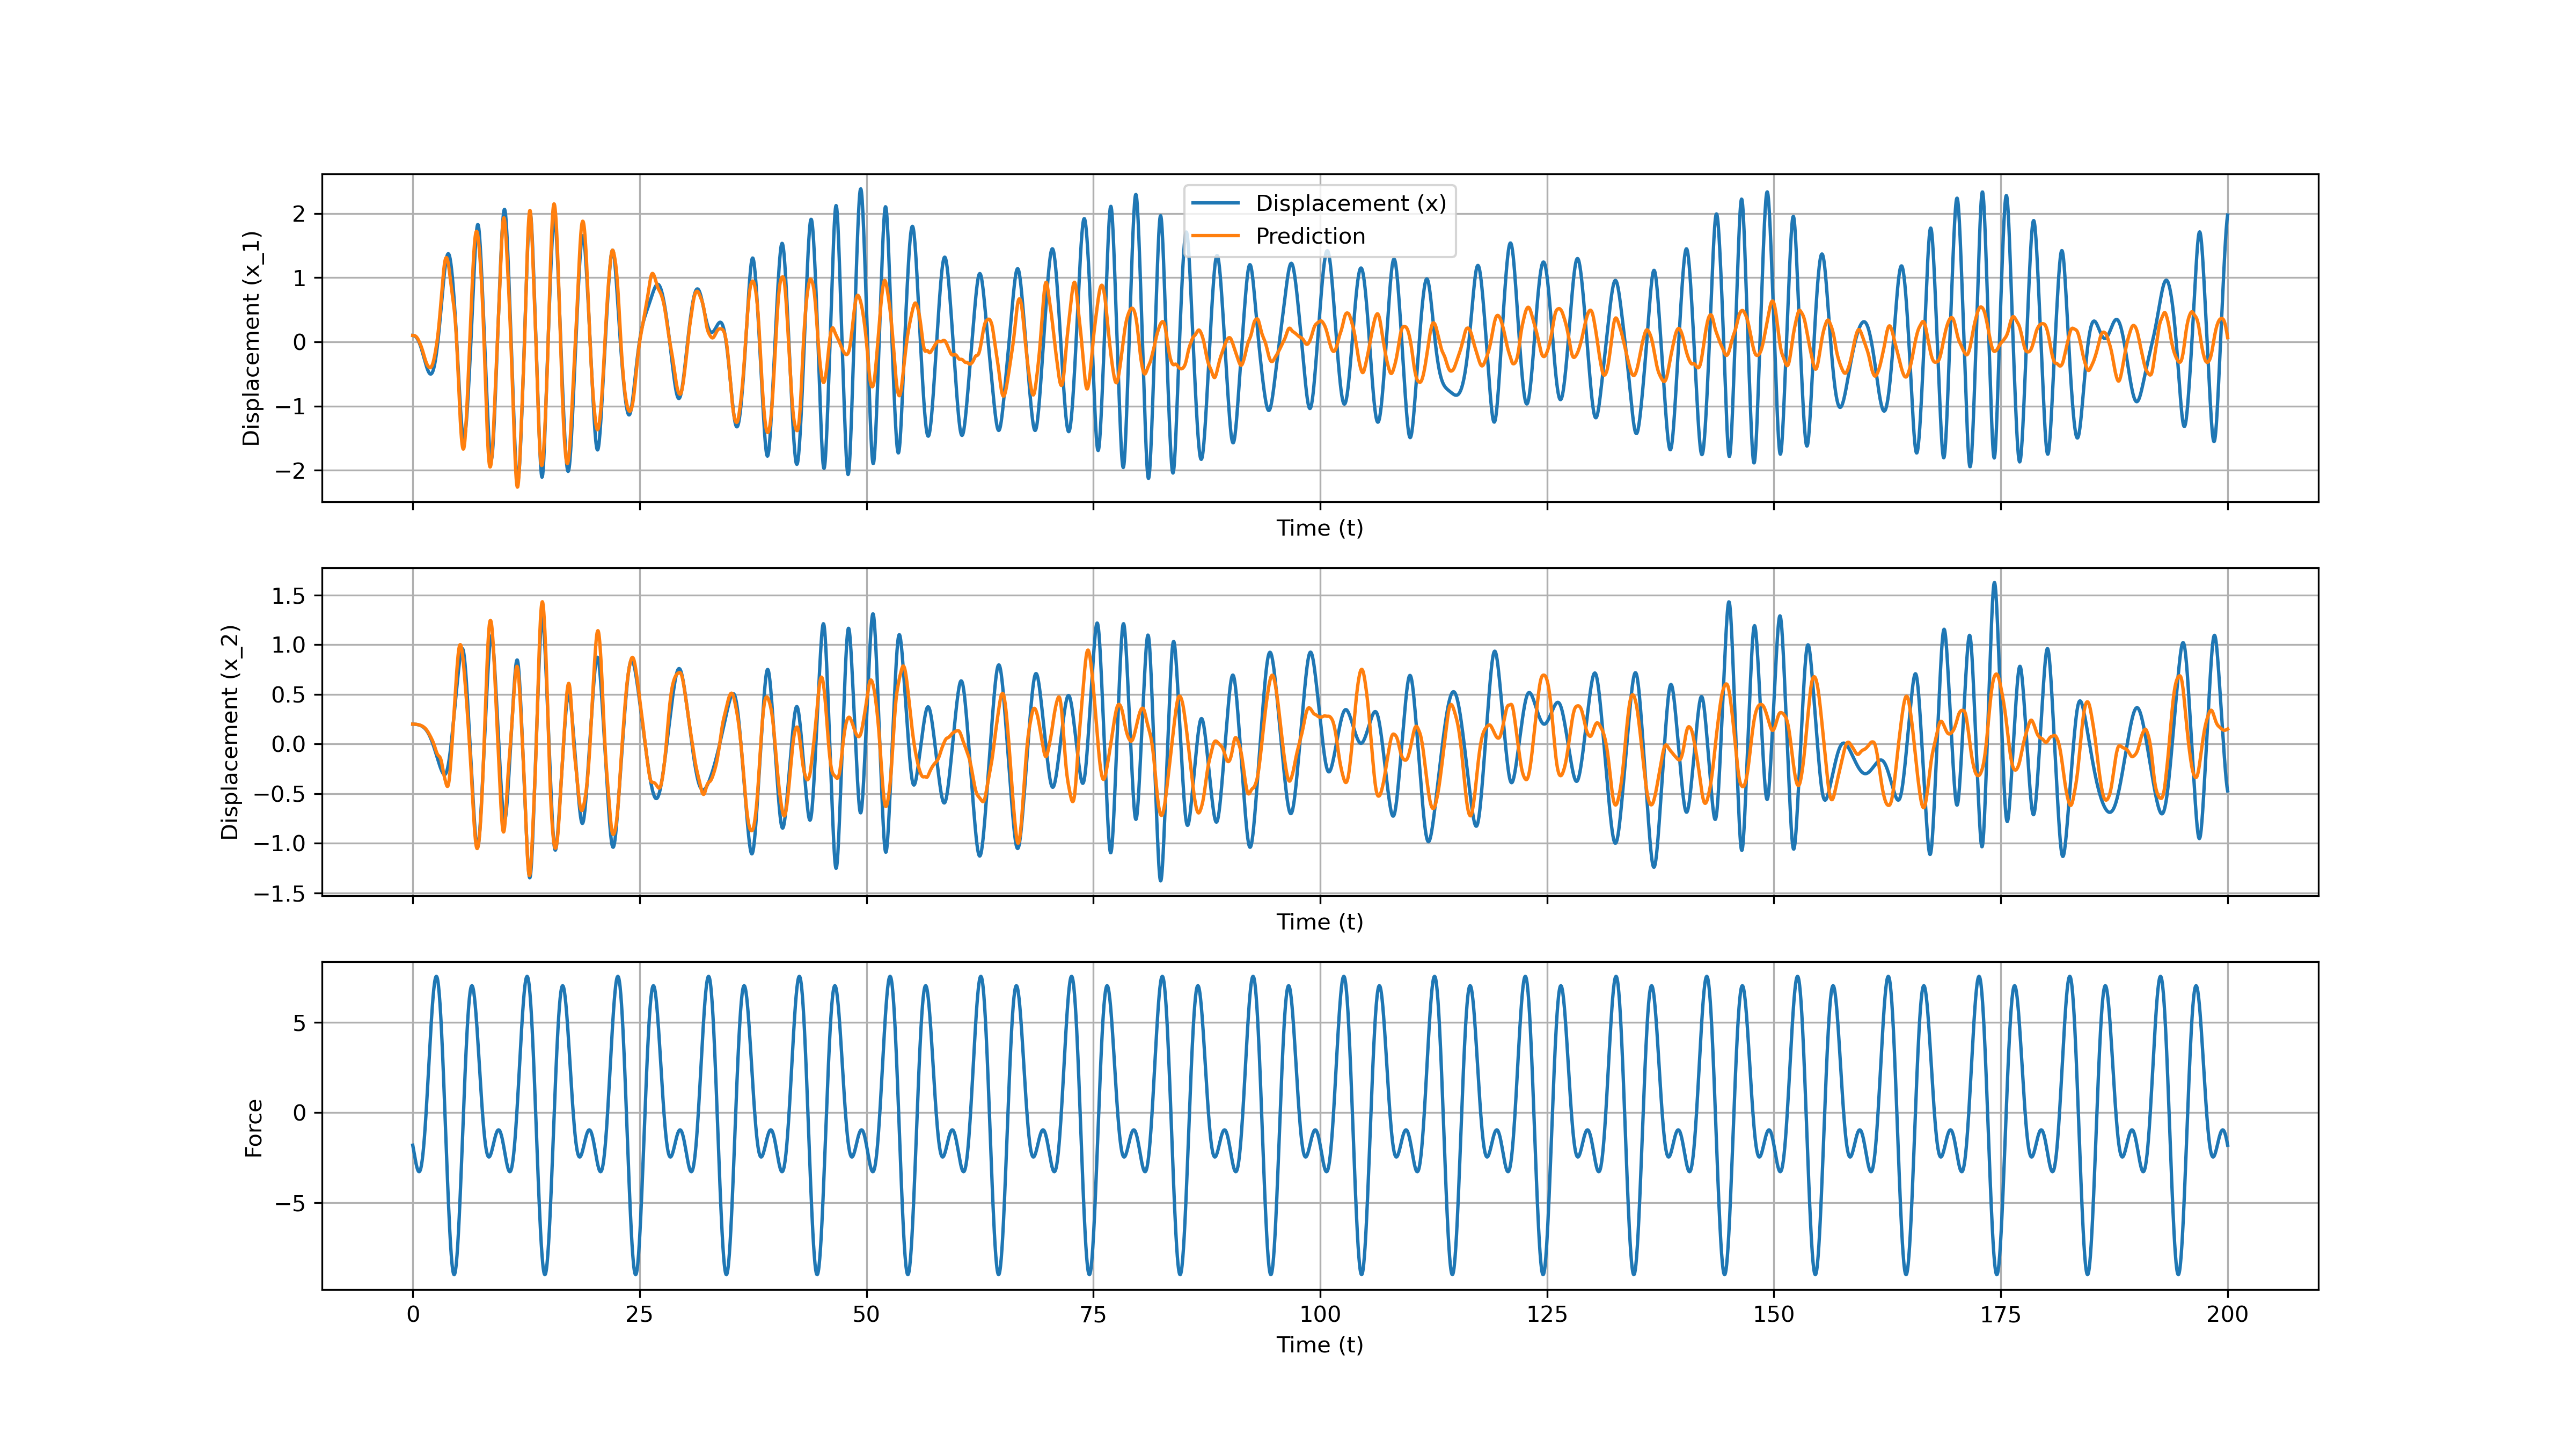
\includegraphics[width=\linewidth]{figures/16384_sobol_2dof_nlinear_tfno.png}
%          \caption{$2^{14}$ dataset testing result}
%          \label{fig:five over x}
%      \end{subfigure}
%         %\caption{Three simple graphs}
%         \label{fig:three graphs}
% \end{figure}

% The second option is using a more complex loss function in order to be able to capture the non-linearity.
% \end{block}
\begin{block}{Test Problem}
\begin{table}[h!]
\centering
\renewcommand{\arraystretch}{2}
\begin{tabular}{
>{\raggedleft\arraybackslash}m{0.2\linewidth} 
>{\centering\arraybackslash}m{0.4\linewidth} 
>{\raggedleft\arraybackslash}m{0.2\linewidth}}

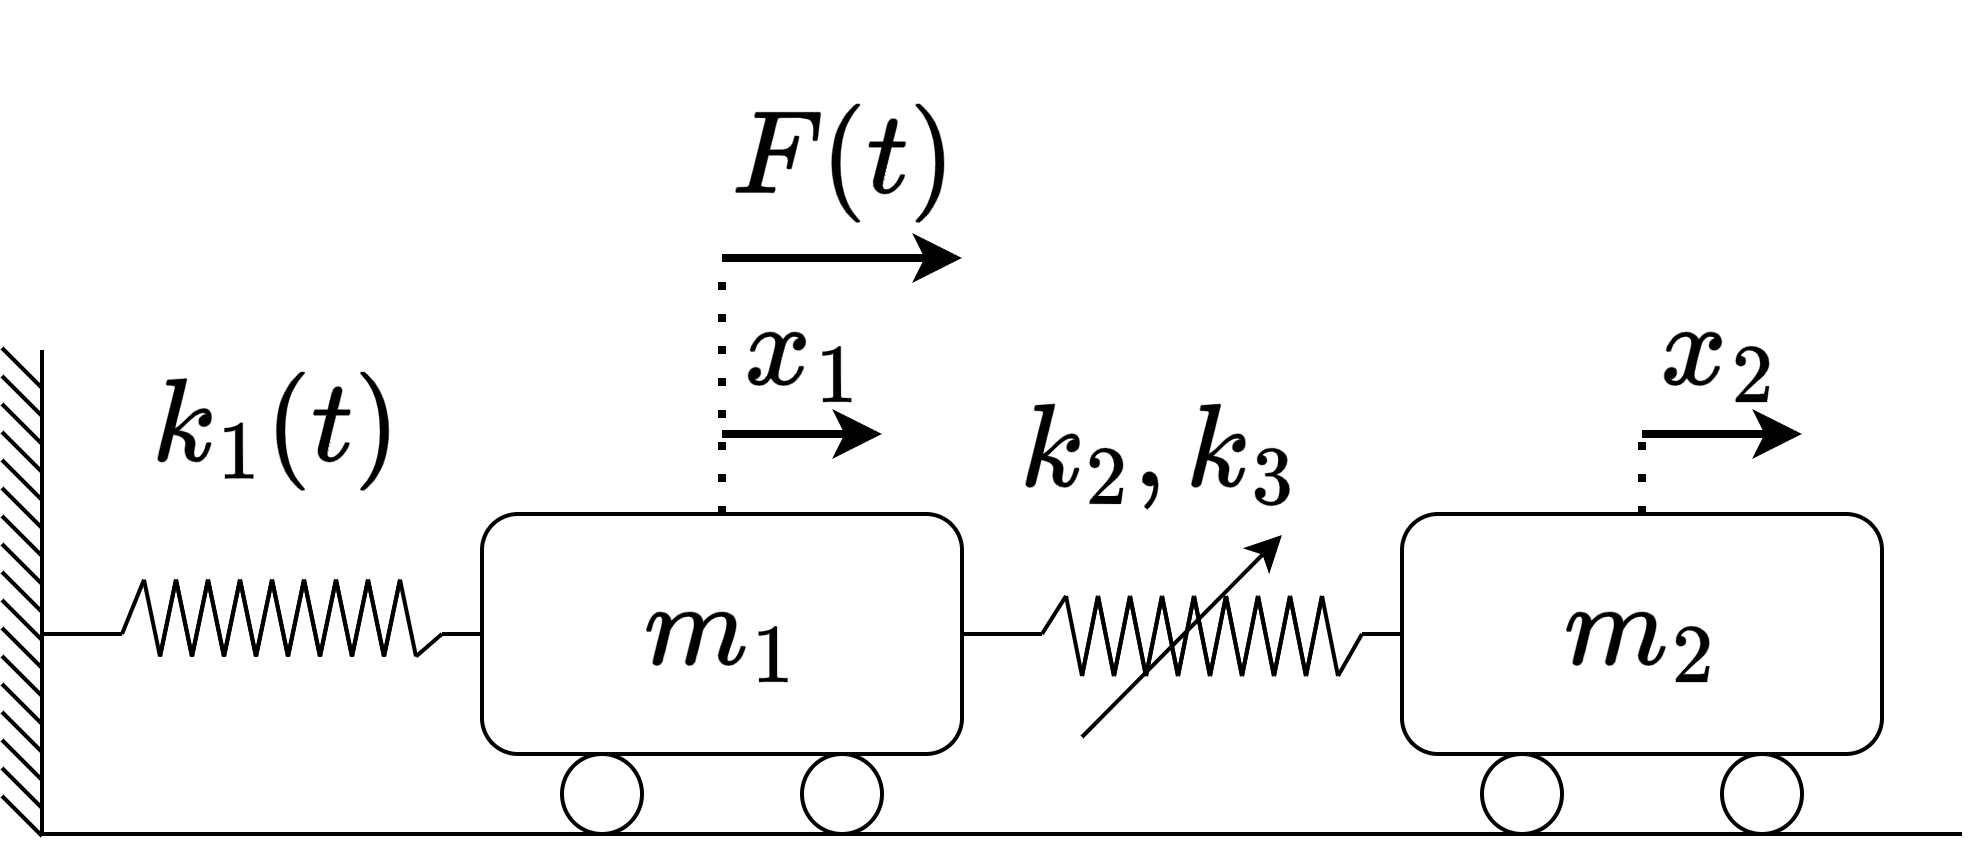
\includegraphics[width=1\linewidth]{figures/2DOF_MassSpring_k1_t.png} &

\(\displaystyle
\begin{aligned}
    &m_{1}\ddot{x}_1 + k_1(t) x_1 + k_2(x_1 - x_2)+ k_3(x_1 - x_2)^3 = F(t) \\
    &m_{2}\ddot{x}_2 + k_2(x_2 - x_1) + k_3(x_2 - x_1)^3 = 0\\
    &k_{1}(t) = k_{0} + k_{initial}e^{-\alpha t}\\
    &F(t) = A\sin(2\pi\omega_1t+\phi_1) + B\cos(2\pi\omega_2t+\phi_2)
\end{aligned}
\) &

\(\displaystyle
\begin{aligned}
    x_1(0) &= 0.1,\:\dot{x}_1(0) = 0 \\
    x_2(0) &= 0.2,\:\dot{x}_2(0) = 0
\end{aligned}
\)
\\
\end{tabular}
%\caption{Figure and two sets of equations: dynamic model and initial conditions.}
%\label{tab:fig_eq_table}
\end{table}
\vspace{0.5cm}
Where  $m_1$ and $m_2$ are 5 and 10 kg, $k_{0}$ is 1 N/m, $k_{initial}$ is 3 N/m while $\alpha$ is 0.01. $k_2$ and $k_3$ are 3 N/m and 2 N/m$^3$. In the forcing function  $\omega_1$ and $\omega_2$ are 0.2 and 0.5 Hz. $A$ and $B$  are sampled from $\mathcal{U}(0,4)$ and $\mathcal{U}(0,5)$ utilizing Sobol's sampling method \cite{sobolDistributionPointsCube1967}, while $\phi_1$ and $\phi_2$  are sampled from $\mathcal{U}(0,2\pi)$. We build the dataset by taking $2^{11}$, $2^{12}$, $2^{13}$ and $2^{14}$ samples from these random variables and then generating the force time series. Afterwards, we solve the 2-DOF system based on those force time series for the displacement of $m_1$ and $m_2$. The equation of motion was solved utilizing \texttt{scipy} Runge-Kutta-Fehlberg Method (RKF45).
\end{block}

\begin{block}{What Has Not Worked? Nonlinear, Non-stationary Systems}
    We tested the FNO with a nonlinear cubic stiffening 2-DOF mass-spring system and time-dependent loading/stiffness parameters. The goal was to test the ability of FNO in predicting the displacement time series of two masses when it gets the force time series as the input. The FNO trained with MSE loss did not function properly in our test. One solution is increasing the size of the datasets. We tested this on $2^{11}$,$2^{12}$,$2^{13}$ and $2^{14}$ dataset sizes. The results show no significant improvement in the results.
    
\begin{figure}
     \centering
     \begin{subfigure}[b]{0.24\linewidth}
         \centering
         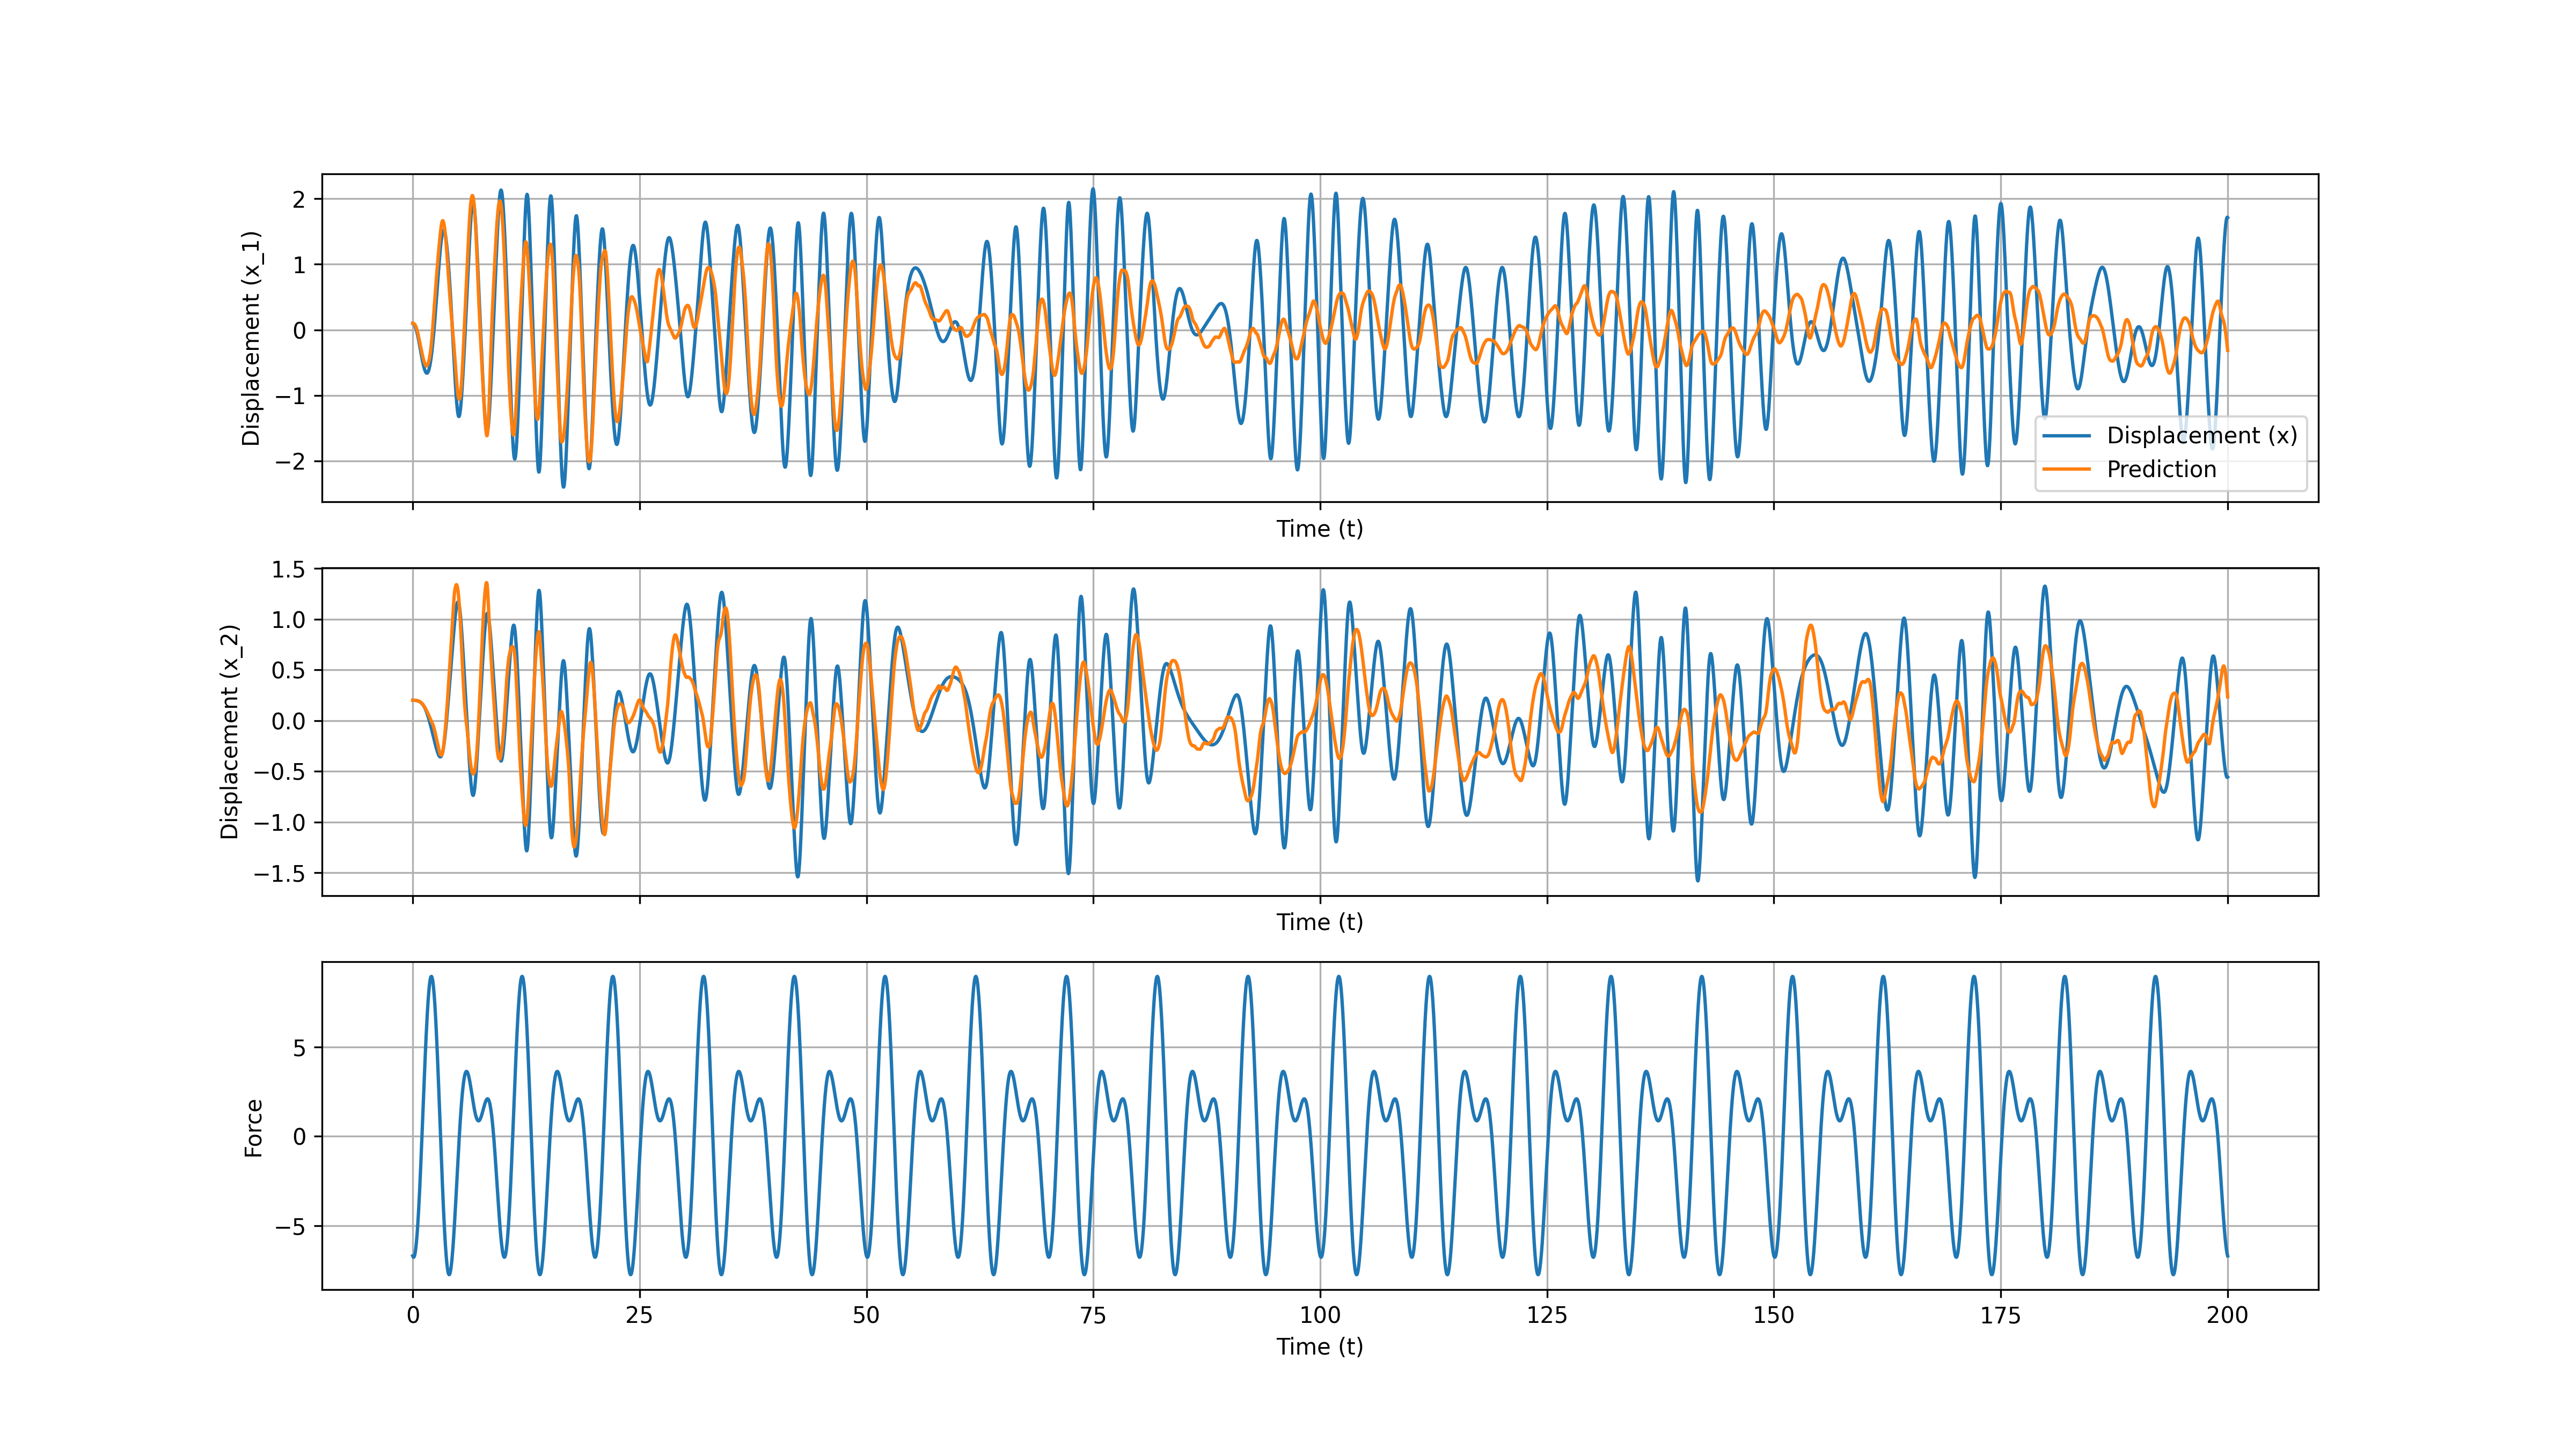
\includegraphics[width=1\linewidth]{figures/2048_sobol_2dof_nlinear_tfno.png}
         \caption{$2^{11}$ dataset testing result}
         \label{fig:y equals x}
     \end{subfigure}
     \hfill
     \begin{subfigure}[b]{0.24\linewidth}
         \centering
         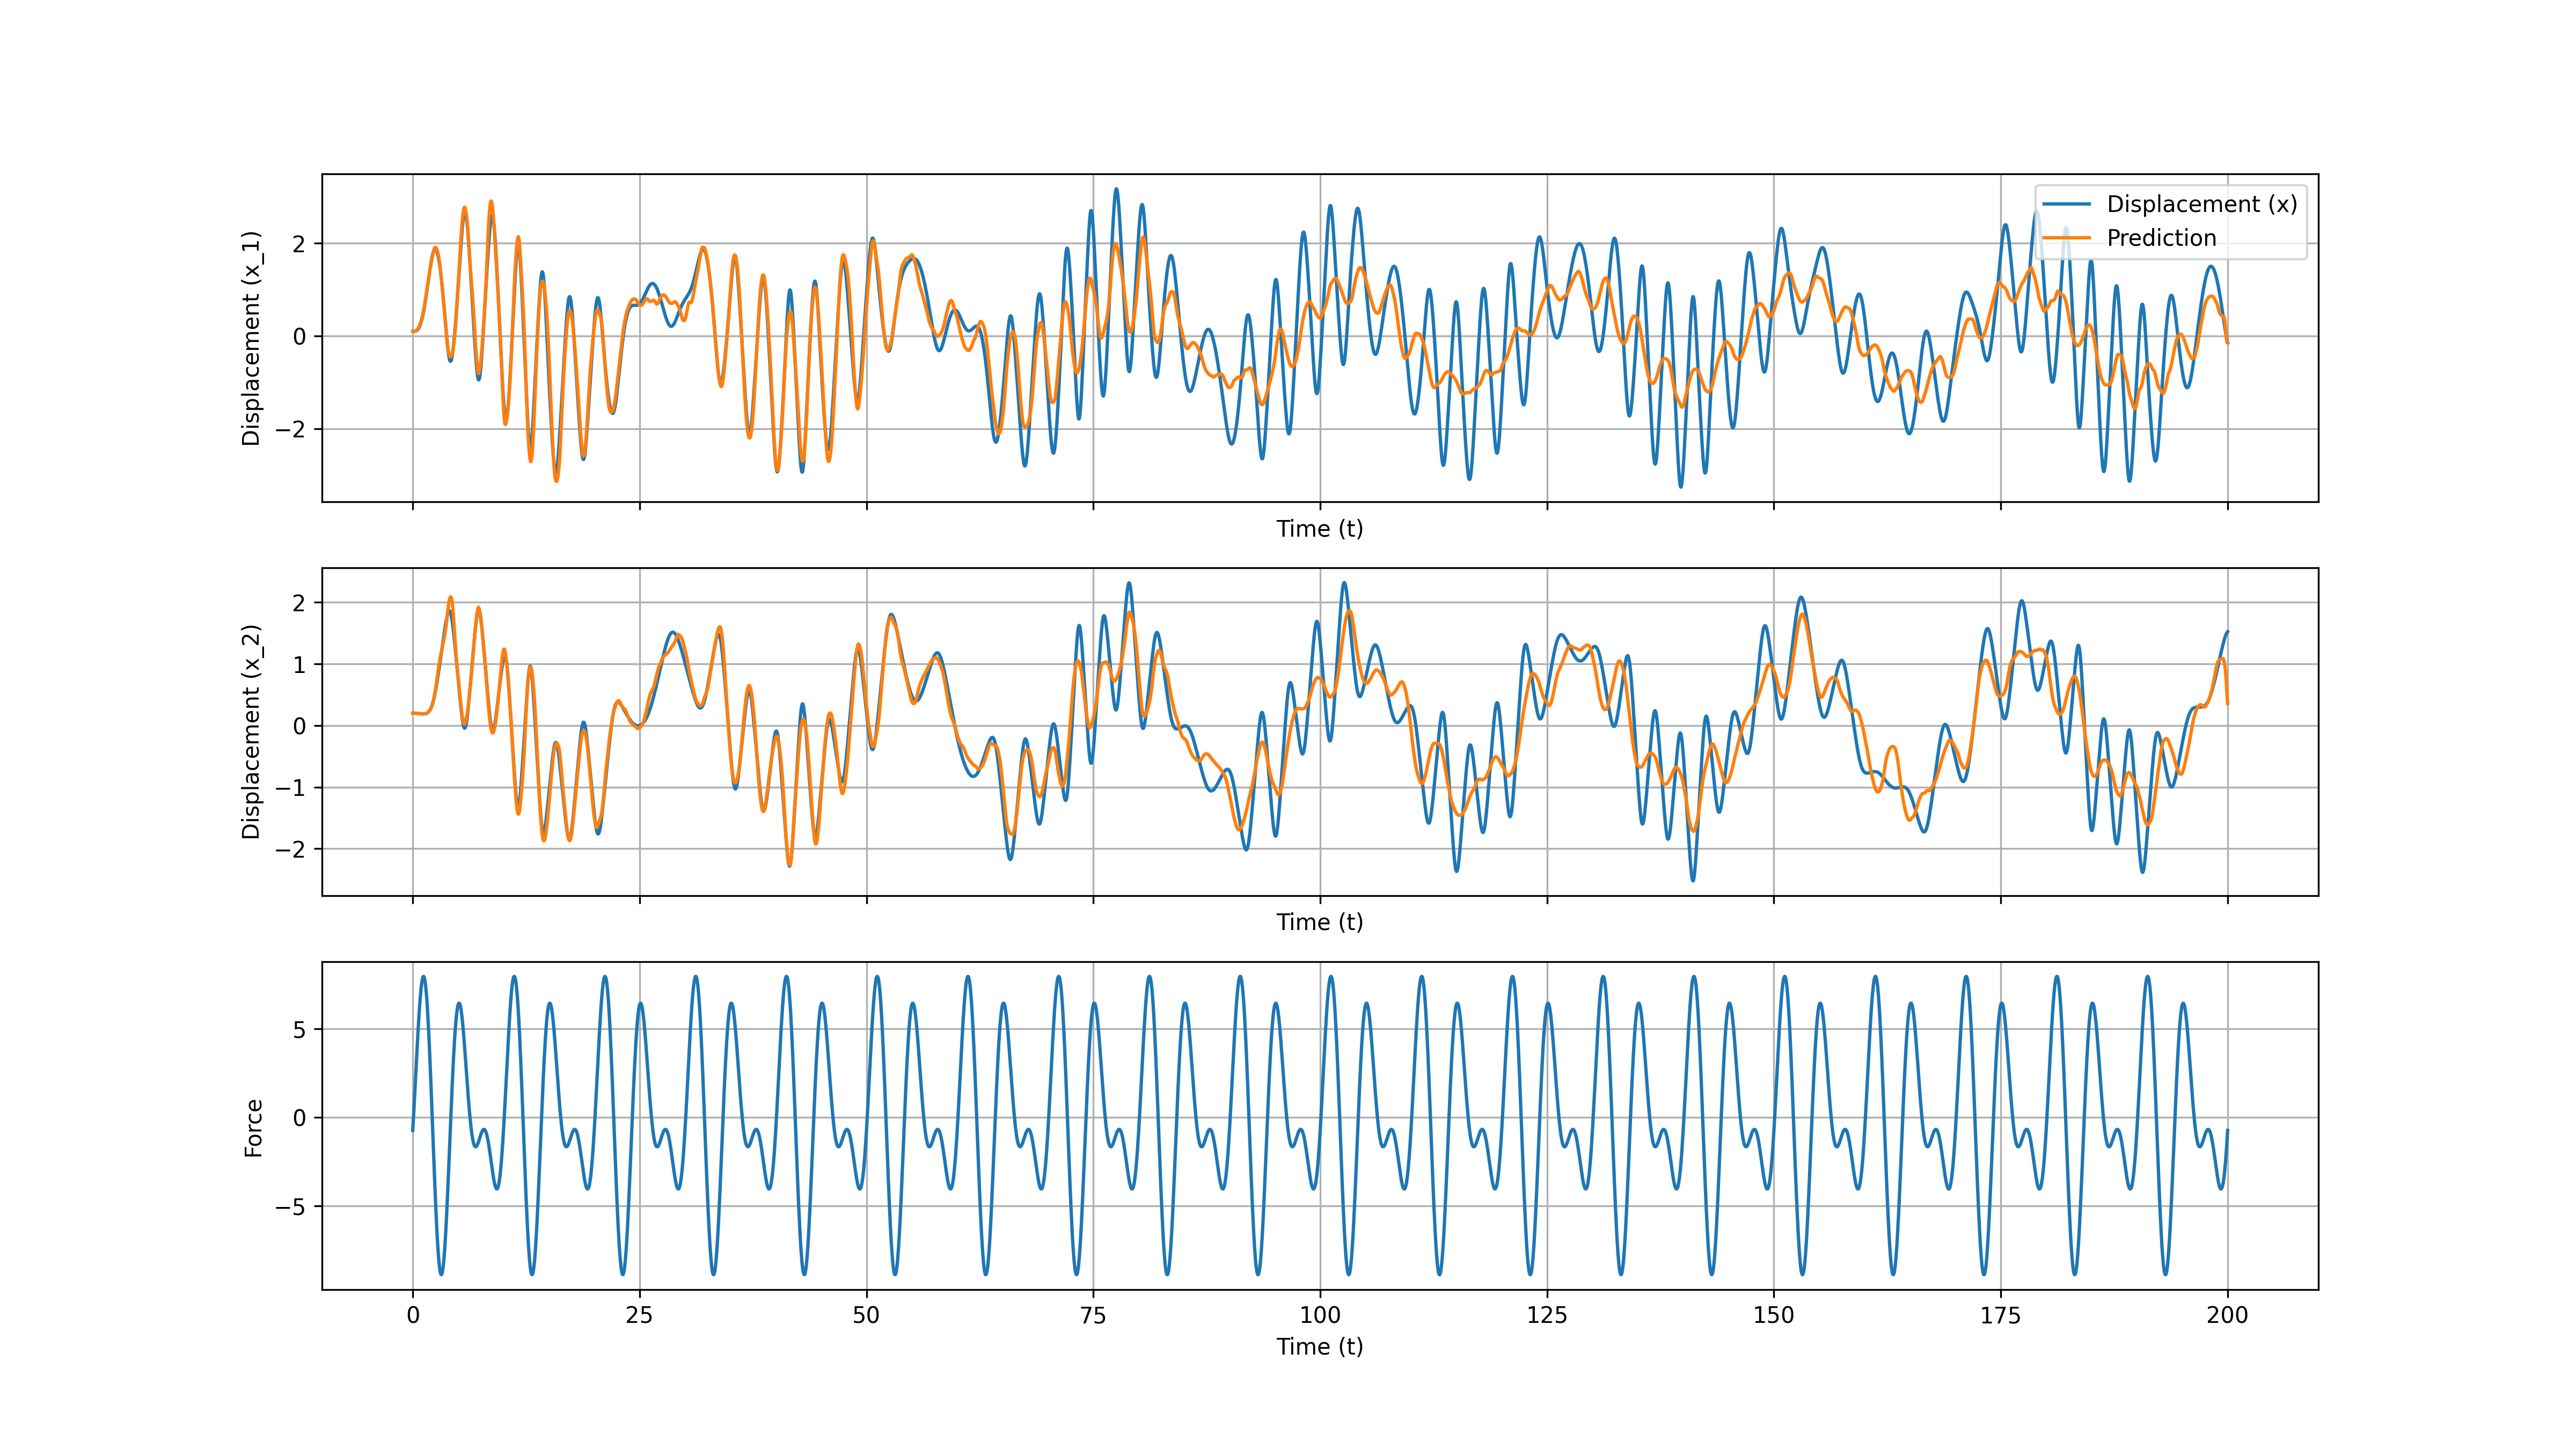
\includegraphics[width=1\linewidth]{figures/4096_sobol_2dof_nlinear_tfno.png}
         \caption{$2^{12}$ dataset testing result}
         \label{fig:three sin x}
     \end{subfigure}
     \hfill
     \begin{subfigure}[b]{0.24\linewidth}
         \centering
         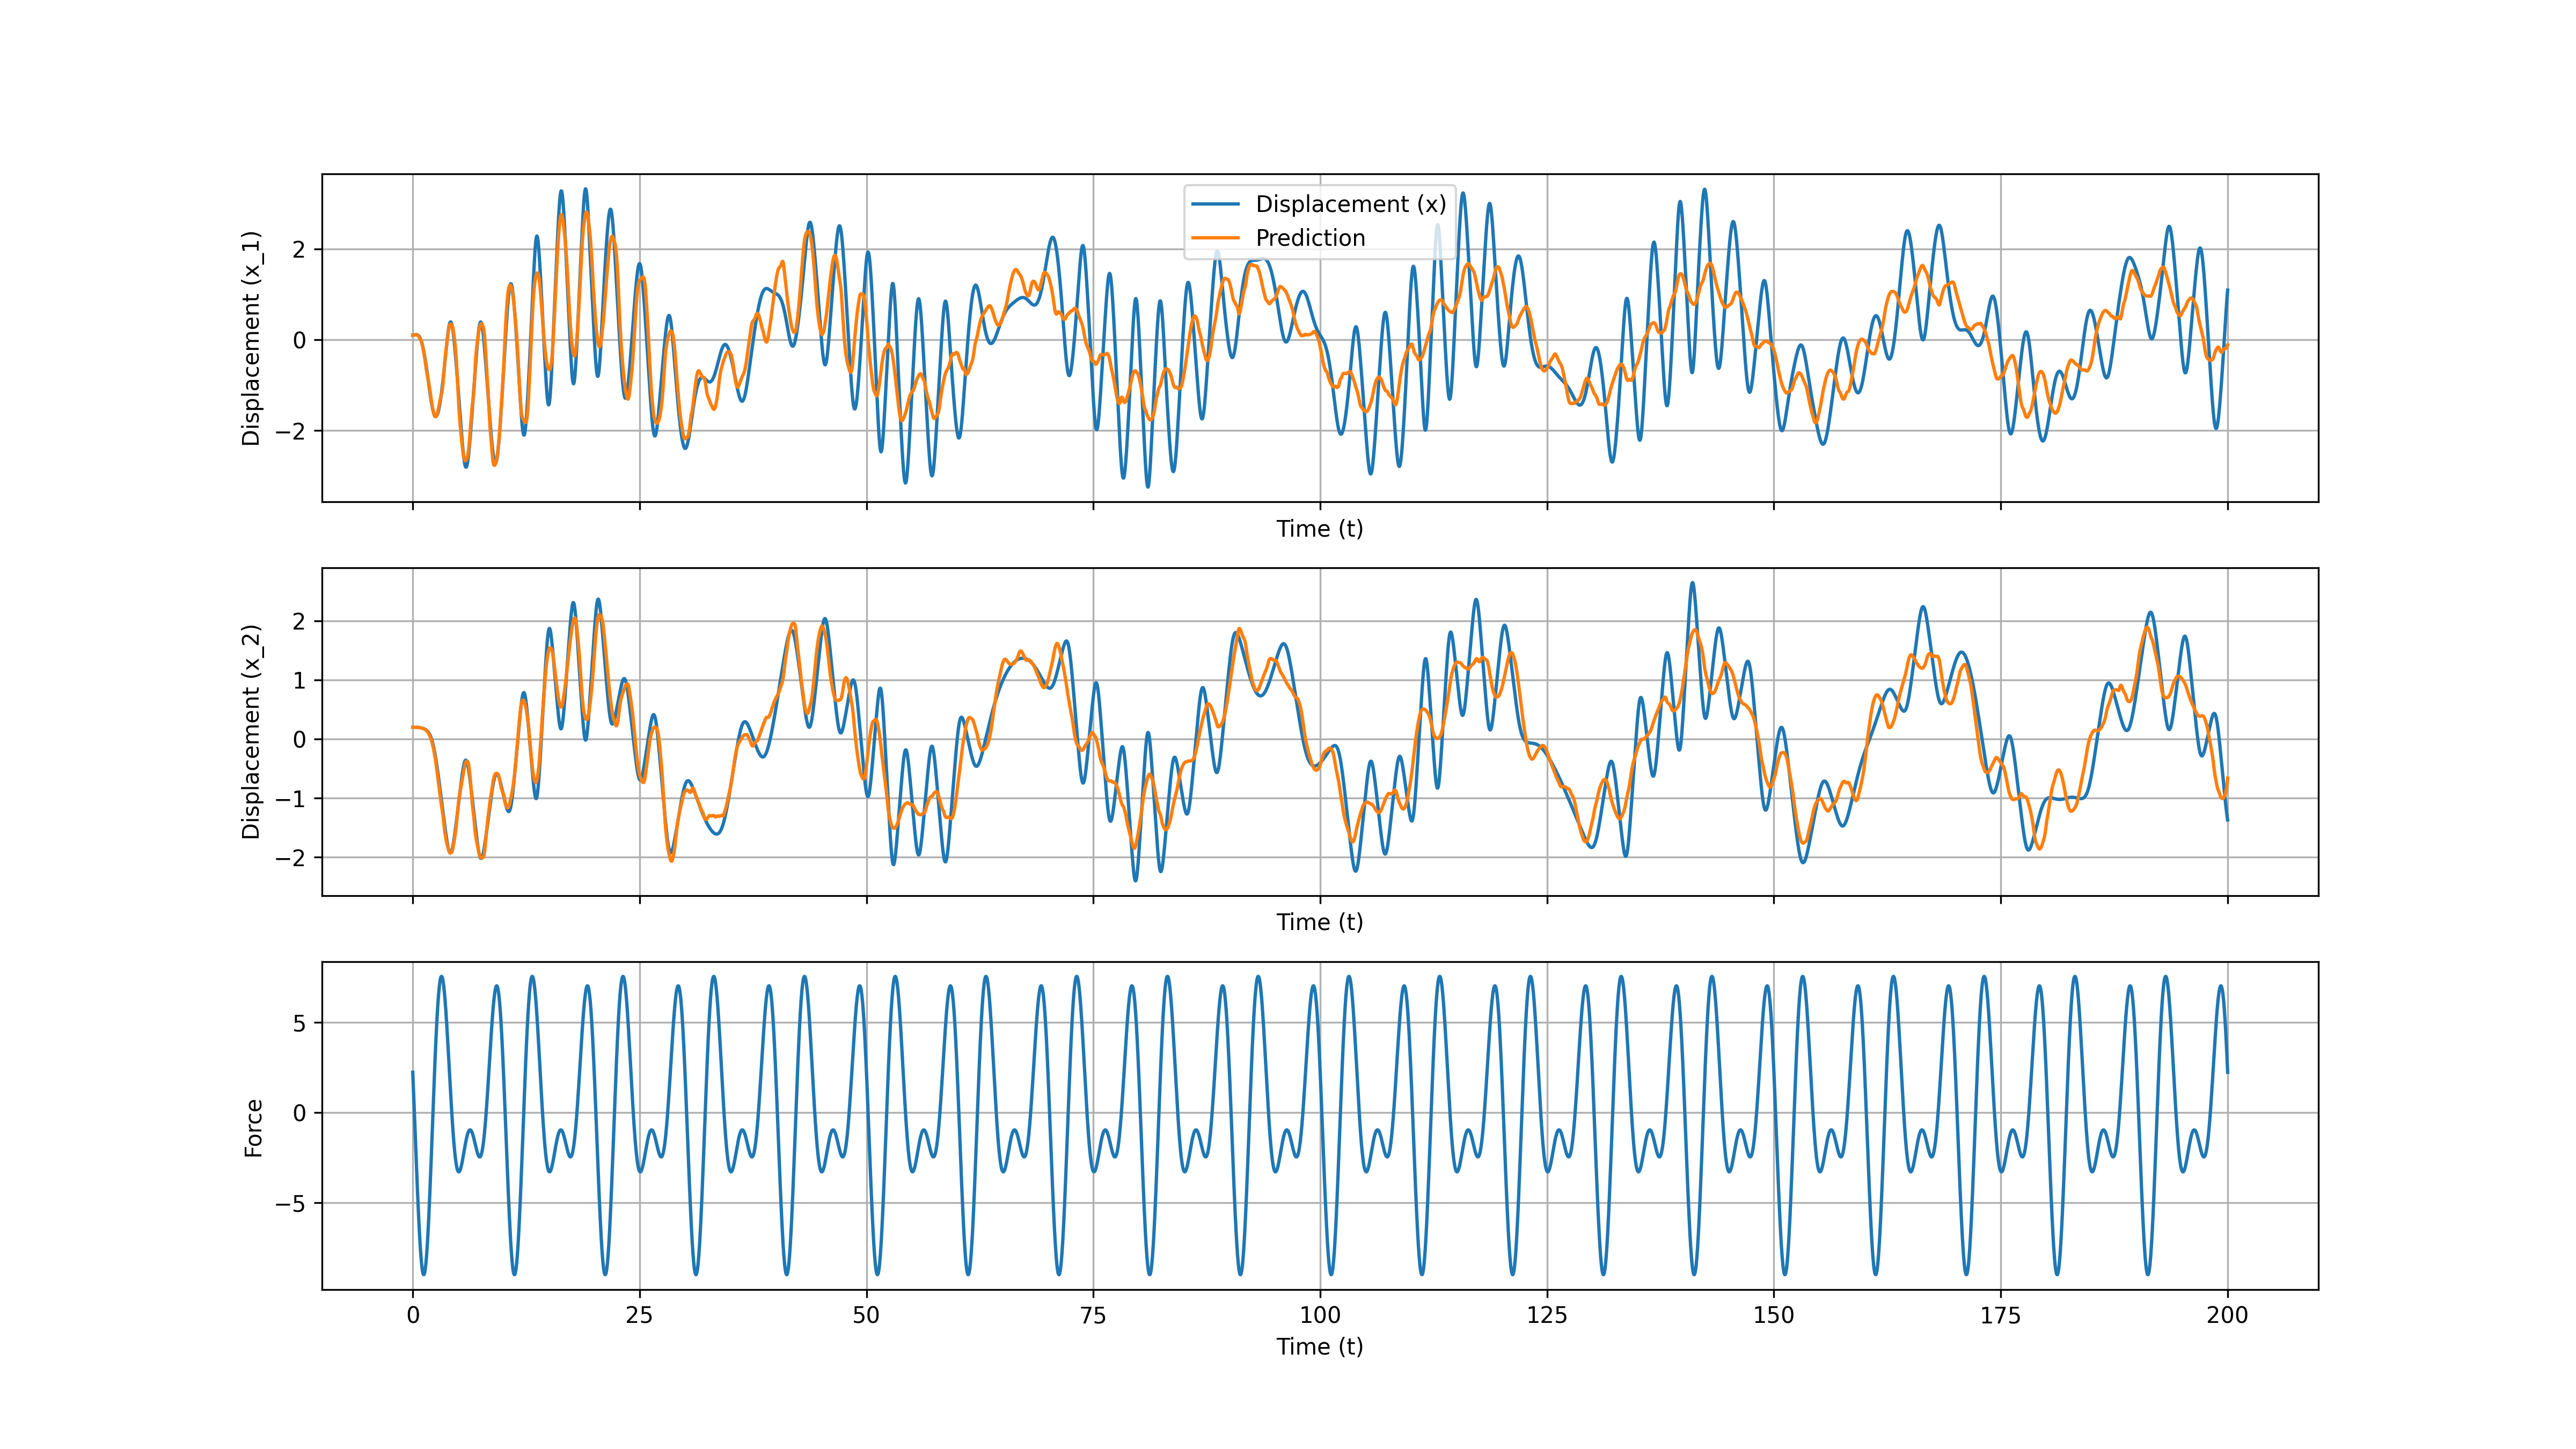
\includegraphics[width=1\linewidth]{figures/8192_sobol_2dof_nlinear_tfno.png}
         \caption{$2^{13}$ dataset testing result}
         \label{fig:five over x}
     \end{subfigure}
     \hfill
     \begin{subfigure}[b]{0.24\linewidth}
         \centering
         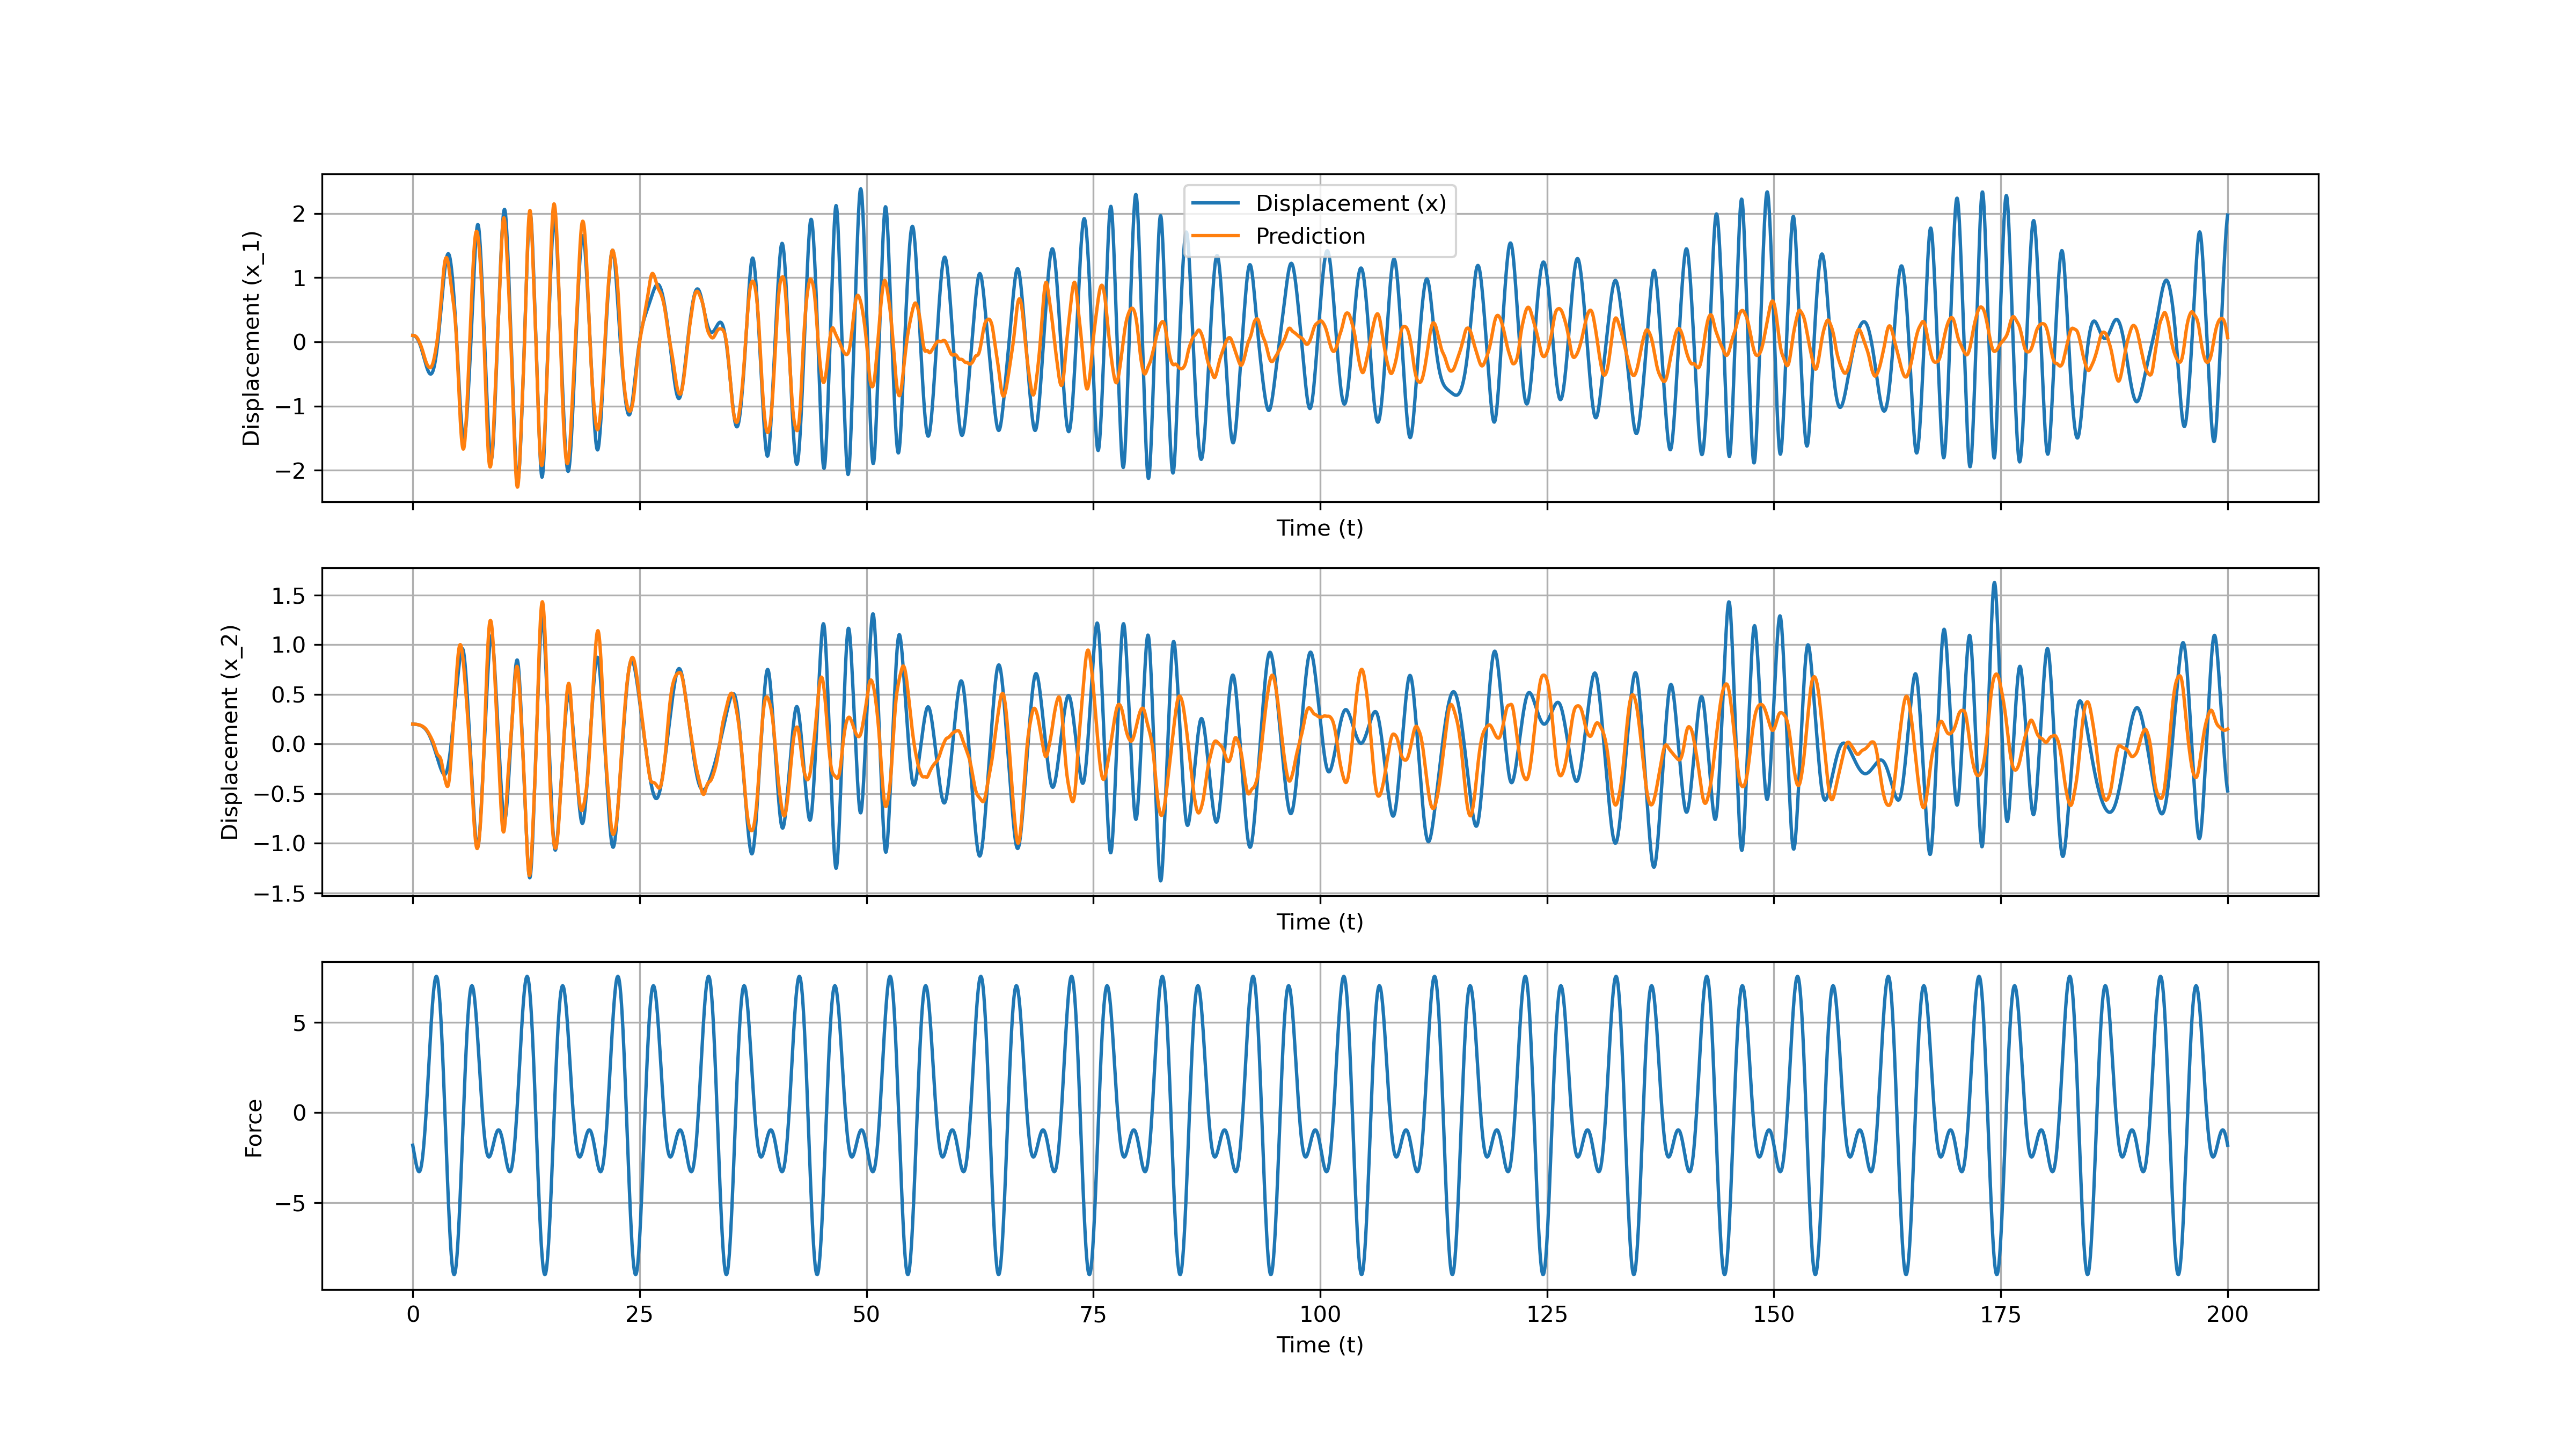
\includegraphics[width=1\linewidth]{figures/16384_sobol_2dof_nlinear_tfno.png}
         \caption{$2^{14}$ dataset testing result}
         \label{fig:five over x}
     \end{subfigure}
        %\caption{Three simple graphs}
        \label{fig:three graphs}
\end{figure}
FNO is able to capture the signal in the initial time steps. However, as the system evolves the prediction worsens. We solve this by designing a novel loss function that can capture the dynamic behavior of the system.
\end{block}



\begin{block}{Spectrogram Loss}
    The Spectrogram Loss compares the frequency content in time of the prediction and ground truth, utilizing short-time Fourier transform (STFT). The loss is calculated for the magnitude of the STFT output. Mathematically it can be defined as:\\

\begin{equation*}
\mathcal{L}_{\text{Spectrogram}} = \frac{\left\| \bm{M}_{\text{pred}} - \bm{M}_{\text{true}} \right\|_F}{\left\| \bm{M}_{\text{true}} \right\|_F + \epsilon}
\end{equation*}
\\
where $\|\cdot\|_F$ is the Frobenius norm. 


%In a flowchart we can show it as the follwoing.
    
%     \begin{figure}
%         \centering
%         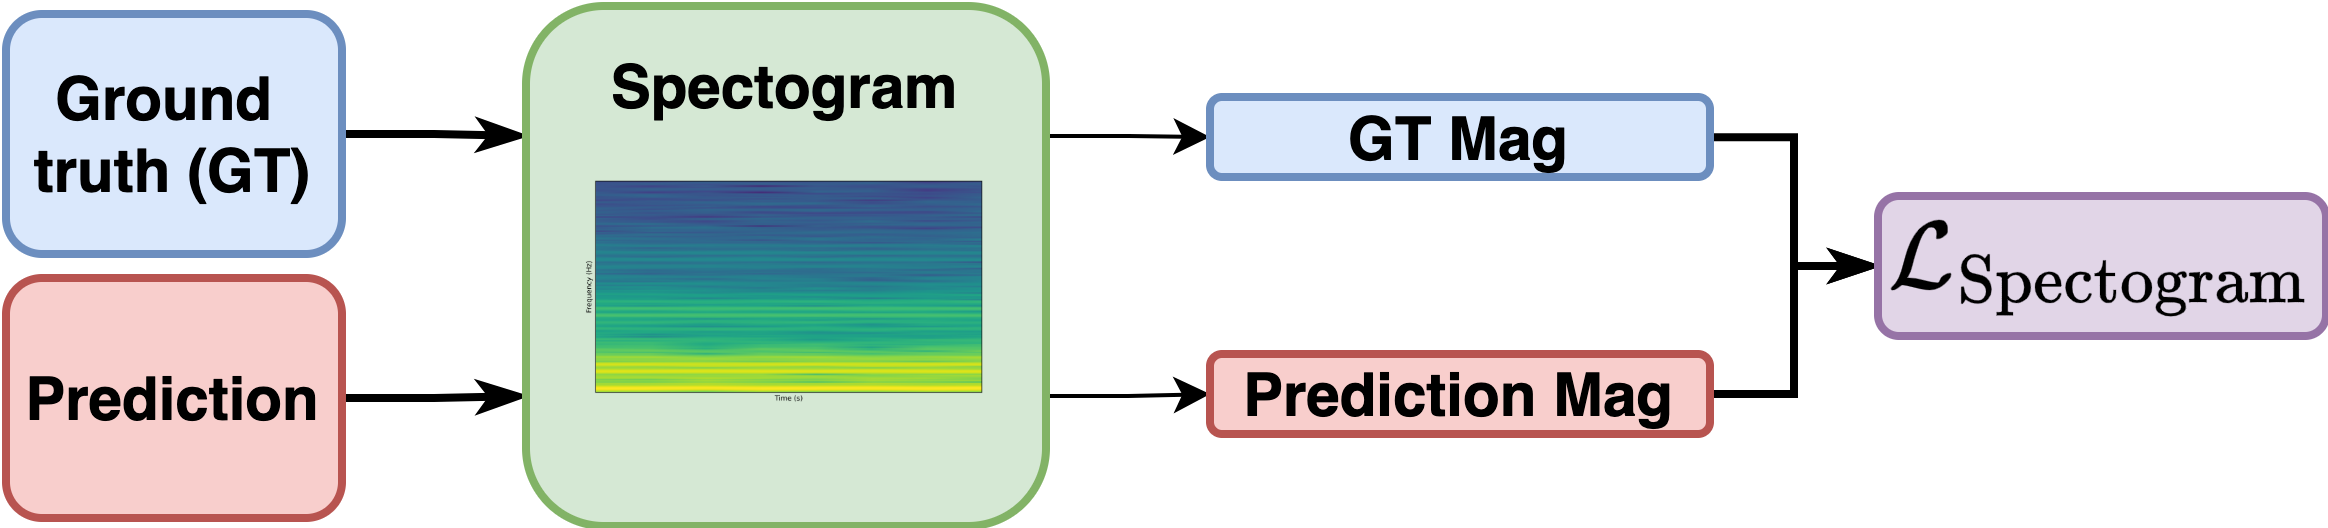
\includegraphics[width=0.5\linewidth]{figures/WESC2025_Abstract-Page-4 (3).png}
%         \caption{Spectogram loss}
%         \label{fig:spec_loss}
%     \end{figure}
 \end{block}


\begin{block}{Results}
We train the 4-layer FNO configurations with two loss configurations on the dataset:

\begin{itemize}
    \item \textbf{FNO1}: four layers FNO, 512 modes, batch size 64, $\mathcal{L} = \mathcal{L_{\text{MSE}}}$
    \item \textbf{FNO2}: four layers FNO, 512 modes, batch size 64, $\mathcal{L} = \lambda_{spectrogram}\mathcal{L_{\text{spectrogram}}} + \lambda_{data} \mathcal{L_{\text{MSE}}}$
\end{itemize}

where $\lambda_{spectrogram}$ is 0.2, and $\lambda_{data}$ is 0.8. The dataset is divided into 80\% for training and 20\% for testing. The results presented below are testing results after 100 epochs.  

\begin{figure}
     \centering
     \begin{subfigure}[b]{0.49\linewidth}
         \centering
         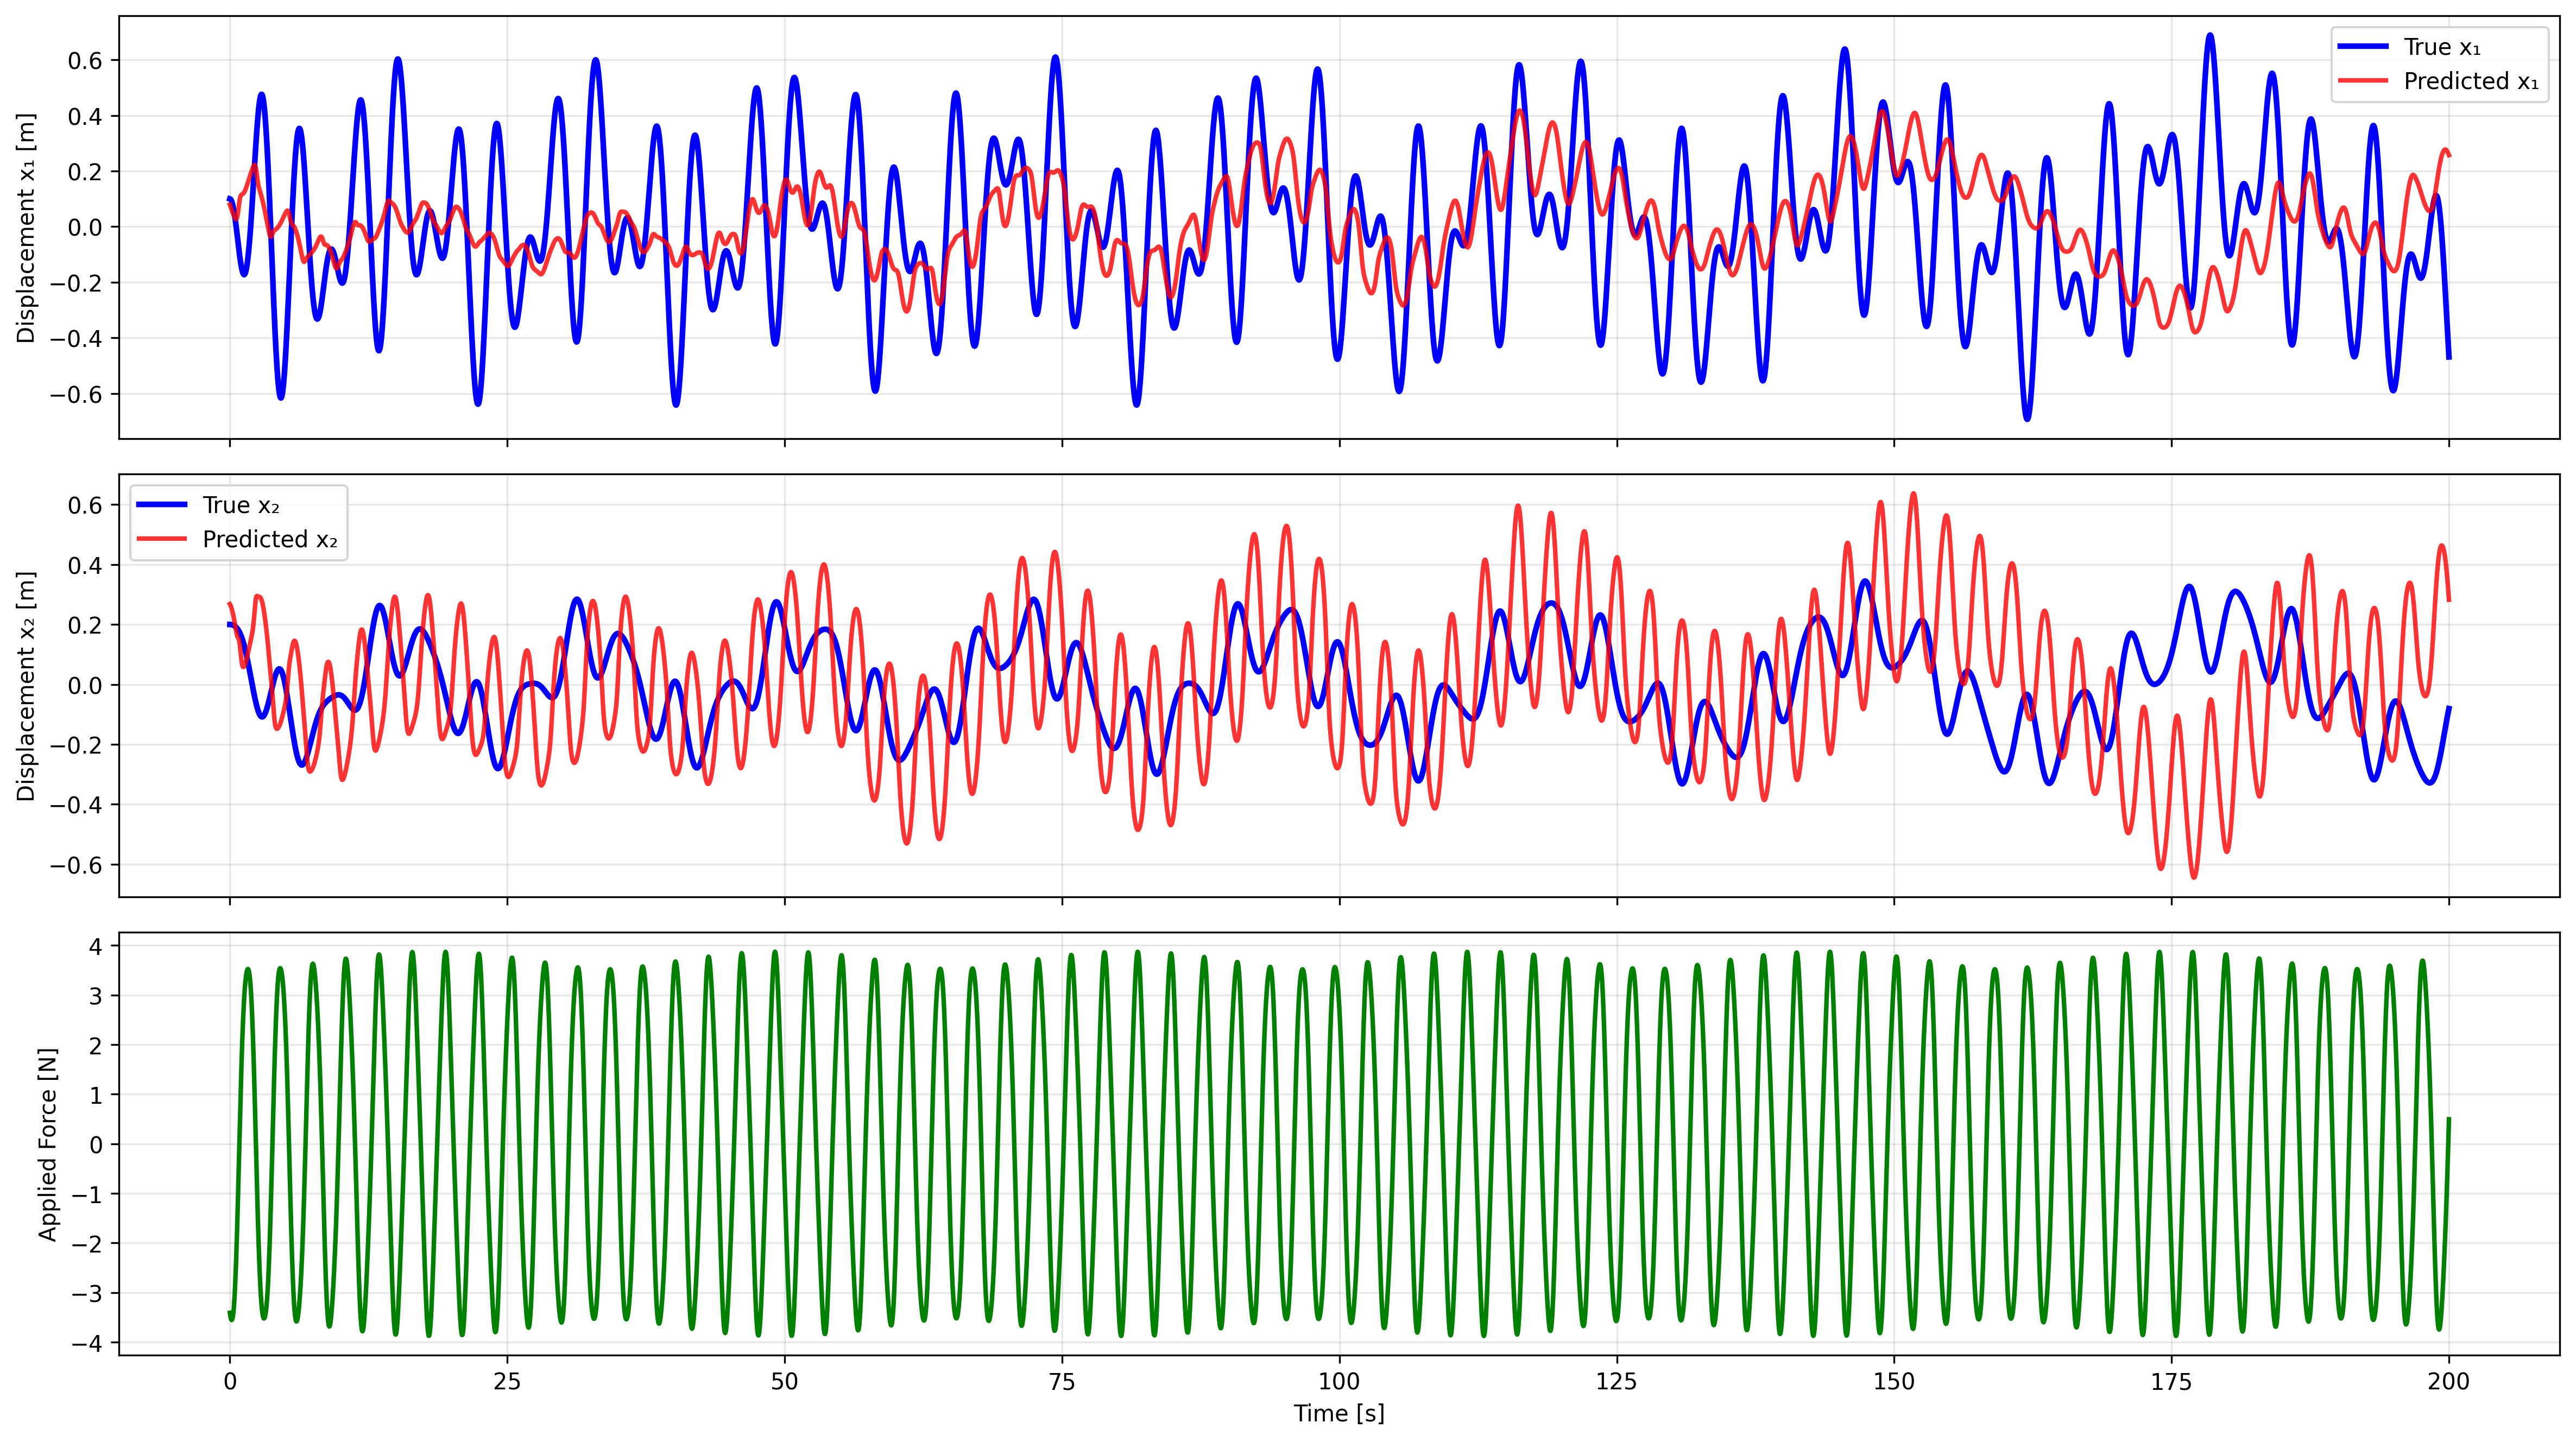
\includegraphics[width=1\linewidth]{figures/0039_0000_TFNO_2dof_nlinear_MSE.png}
         \caption{FNO1: $\mathcal{L_{\text{MSE}}}$}
         \label{fig:y equals x}
     \end{subfigure}
     \hfill
     \begin{subfigure}[b]{0.49\linewidth}
         \centering
         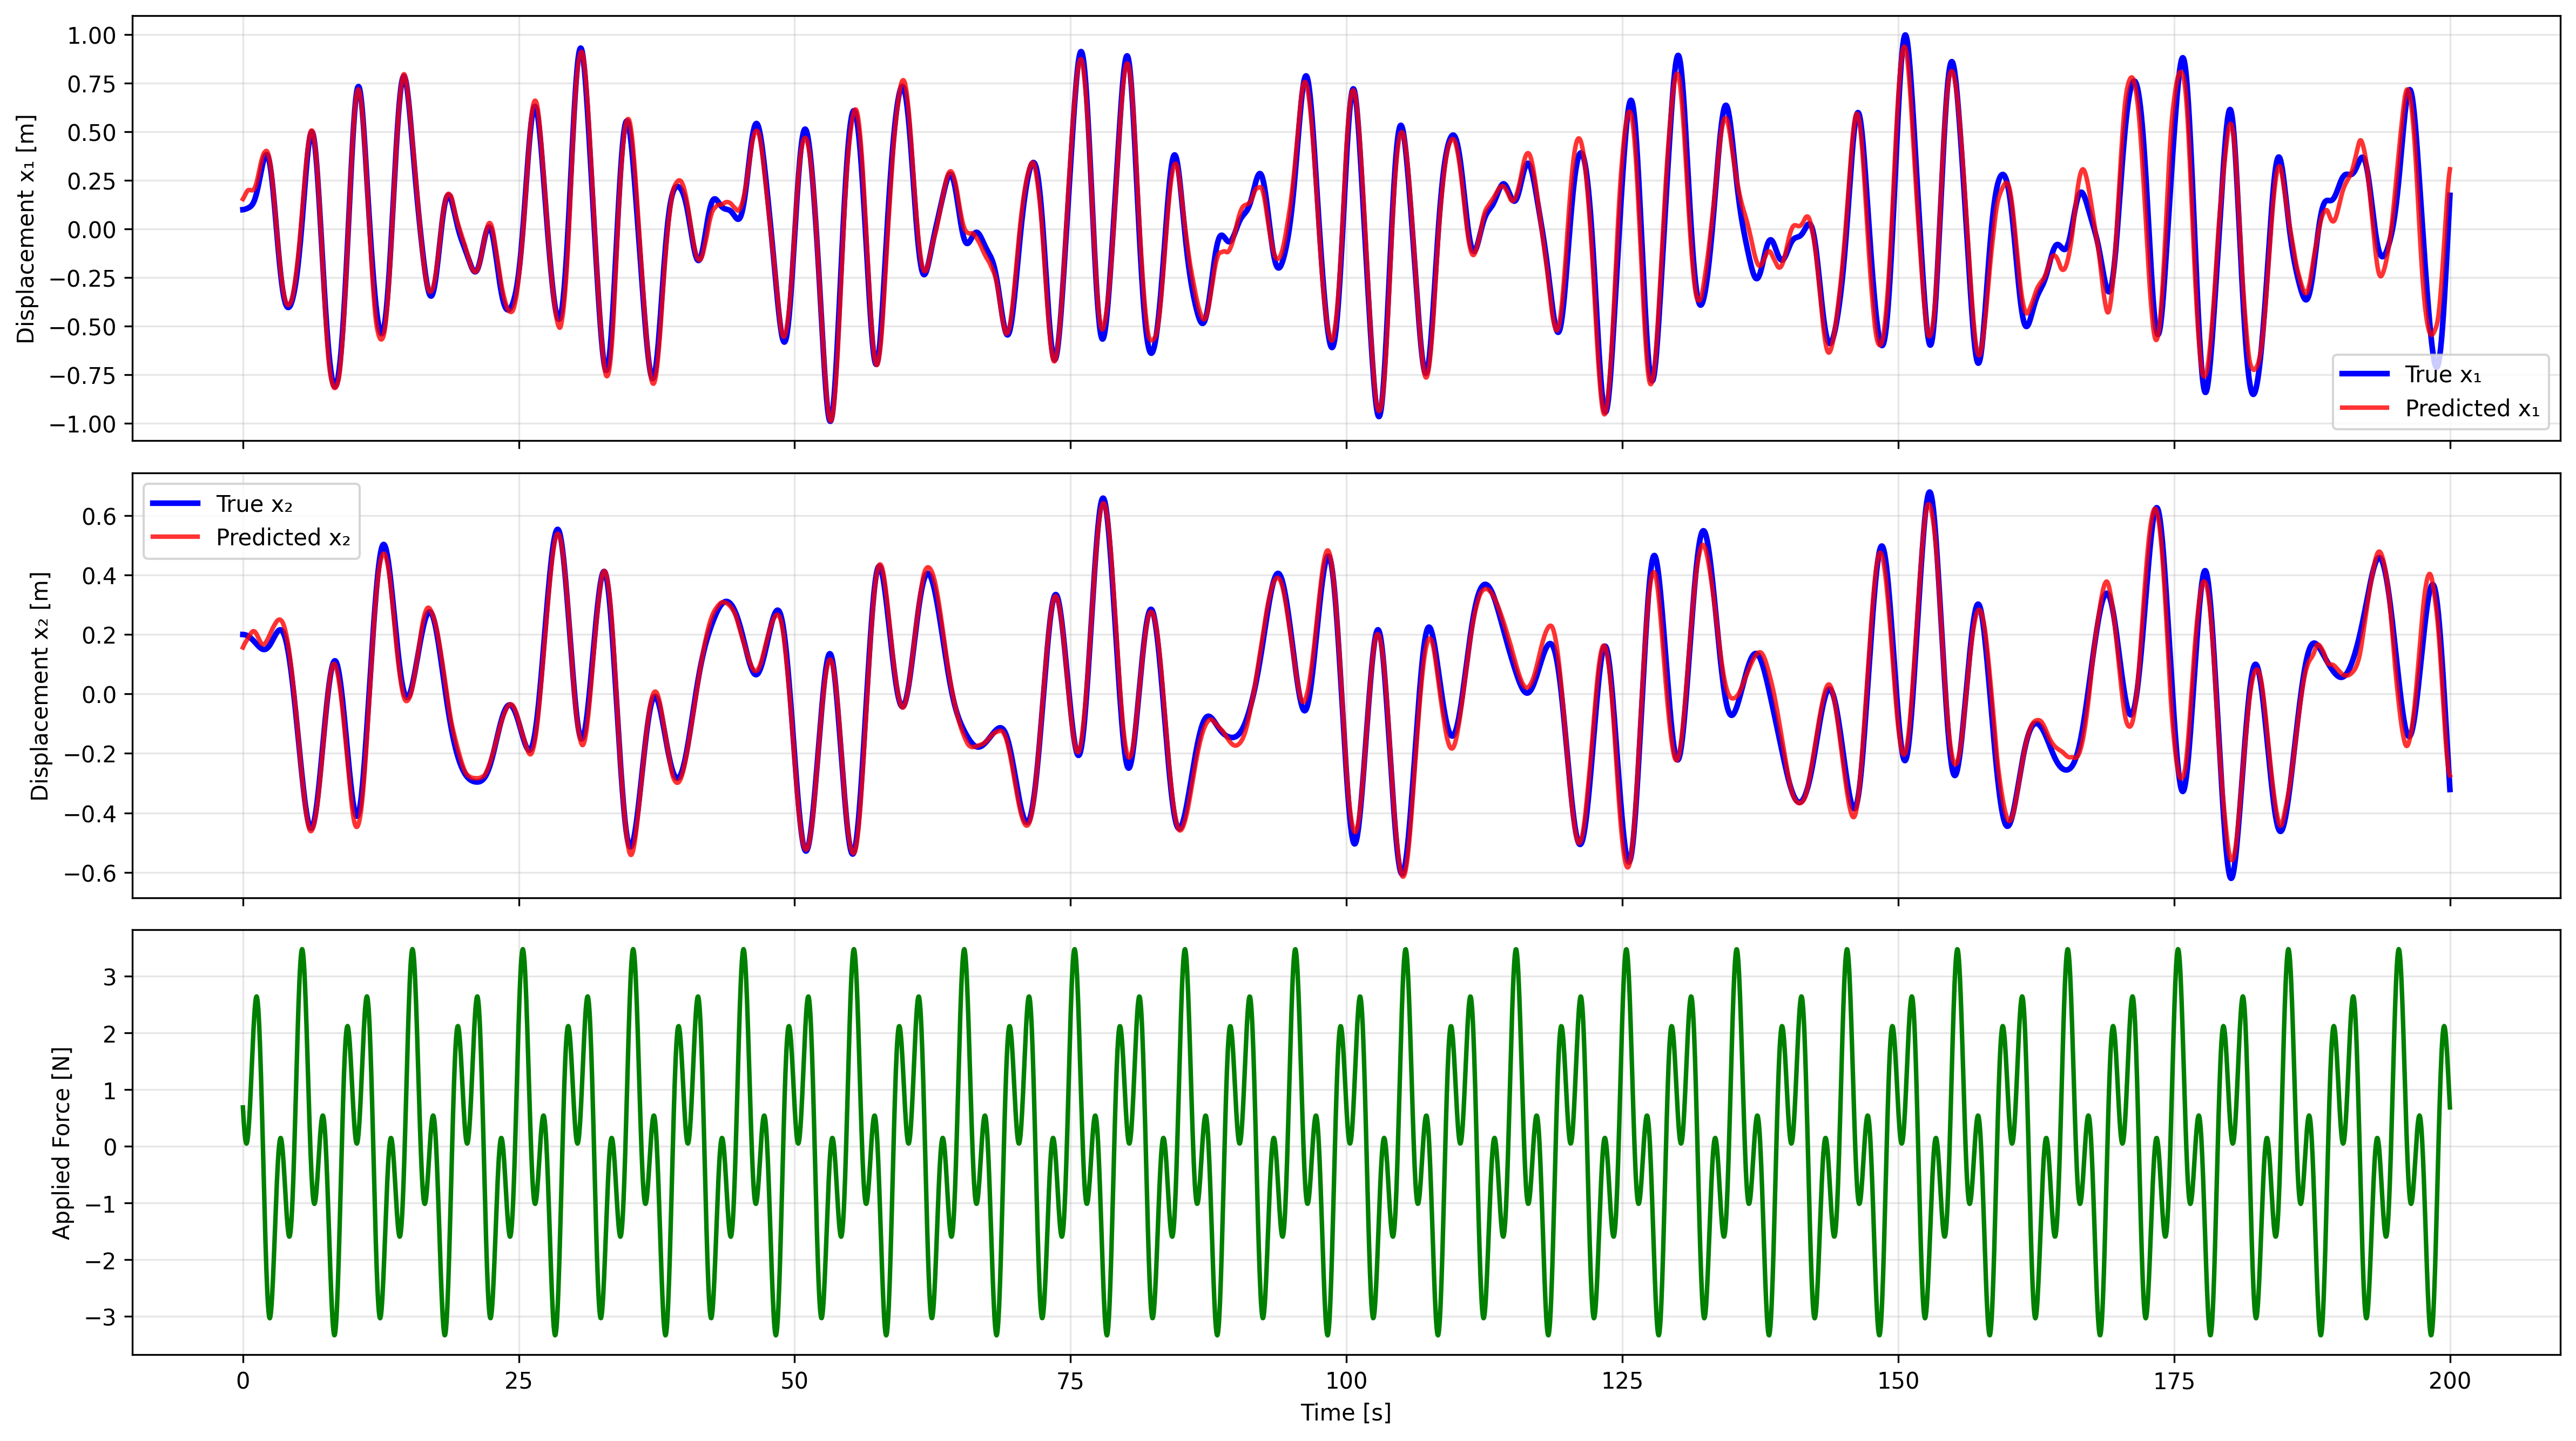
\includegraphics[width=1\linewidth]{figures/TFNO_2dof_nlinear_softening_k1_spectral.png}
         \caption{FNO2: $\mathcal{L} = \lambda_{spectrogram}\mathcal{L_{\text{spectrogram}}} + \lambda_{data} \mathcal{L_{\text{MSE}}}$}
         \label{fig:three sin x}
     \end{subfigure}
\end{figure}

The FNO with the spectrogram loss has a clear advantage in being able to capture the changes in the system over time. We compare the frequency content of the prediction vs. the actual by running the spectrogram on all the 20\% test part of the dataset, and also on the corresponding predictions. 



% \textbf{Drawback:} We tested FNO with Spectrogram loss on a dataset that the frequency of the force time series was also coming from two uniform distribution. The rest of the process stayed the same. Our tests showed this setup did not reach low error in both training and testing. This means this setup works with one changing frequency content (in this case the frequency changes in the system), however the combination of the frequency changes in both input and the system needs further investigation. {\bf Unclear! remove?}

\end{block}		
% \noindent where A is constant, and To build the databases, we took $2^{10}$, $2^{11}$, $2^{12}$ and $2^{13}$ samples from the uniform distributions for the phase in Eq. \eqref{eq:force} and solves linear and nonlinear systems to find the displacement time series for $x_1$ and $x_2$. This provided us with four databases with different numbers of samples. The goal here is to investigate the impact of sample size on both training and testing as well. The system and forcing function properties can be found in Table \ref{tab:systems_prop}.      




%\end{block}	


    }
\end{minipage}
\end{beamercolorbox}


%----------------------------------------------------------Right Column ---------------------------------------------------------------


		\column{.25\textwidth}
		\begin{beamercolorbox}[center,wd=\textwidth]{postercolumn}
			\begin{minipage}[T]{.95\linewidth}  % tweaks the width, makes a new \textwidth
			     \parbox[t][\columnheight]{\textwidth}{ % must be some better way to set the the height, width and textwidth simultaneously
			      % Since all columns are the same length, it is all nice and tidy.  You have to get the height empirically
\begin{figure}
    \centering
    \includegraphics[width=1\linewidth]{figures/spectrogram_comparison_2x3_avg (3).png}
    \caption{The average spectrogram on the 20\% test}
    \label{fig:enter-label}
\end{figure}

The presented error is based on the difference in the power spectrum. This shows a good match between the prediction and actual frequency content. The spectrogram loss works here as it pushes the training algorithm to take into account the time-varying frequency components, where they are not taken into account with the MSE loss. This gives the FNO the ability to digest the nonlinear time-varying system.\\



\begin{block}{Conclusion and Discussion}

\begin{itemize}
    \item Out-of-the-box FNO with MSE loss works well for a linear system. We showed the capabilities of FNO on a linear 2-DOF and an OWT simulation outputs.
    \item The same architecture could not achieve desirable accuracy regardless of the training dataset size when the model is nonlinear. We showed this by training the FNO on four different sizes of datasets.
    \item As the option of increase in the dataset size did not work, and the results show further inclusion of the frequency is required, we added the spectrogram loss to the FNO.
    \item The FNO with spectrogram loss showed improvement predicting the nonlinear time-varying 2-DOF mass-spring system.
    \item Our tests show if the input force has changing frequency in the dataset, the training and testing error will not reach to an acceptable level. This needs further investigation.
    \item Calculating spectrograms is computationally expensive, especially when it adds up in a training process. Improvement on that front needs further investigation.
\end{itemize}

\end{block}
			
\begin{block}{Future Work Questions}
\begin{itemize}
    \item How can the FNO setup with spectrogram loss performance be improved for systems where the frequency content of the forcing function is changing?
    \item What is the prediction of the trained FNO model when the forcing function is out of the training dataset? How can we improve it?
    \item What other loss functions can help FNO capture the dynamic frequency content? Which are computationally less expensive?
\end{itemize}
\end{block}
				
				 \begin{block}{Acknowledgement}
			The authors acknowledge the Tufts University High Performance Compute Cluster \url{https://it.tufts.edu/high-performance-computing} which was utilized for the research reported in this paper.
				 \end{block}
				 
				 
				 \begin{block}{References}
				%Put your references here --{\bf Use shorter refs.}
                    \bibliographystyle{abbrvnat}
					\bibliography{A0Poster.bib}
%					\vskip .72em
				 \end{block}
				 }
			\end{minipage}
		\end{beamercolorbox}
	\end{columns}
	
 
\end{frame}
\end{document}


%%%%%%%%%%%%%%%%%%%%%%%%%%%%%%%%%%%%%%%%%%%%%%%%%%%%%%%%%%%%%%%%%%%%%%%%%%%%%%%%%%%%%%%%%%%%%%%%%%%%
%%% Local Variables: 
%%% mode: latex
%%% TeX-PDF-mode: t
%%% End:


\textcolor{red}{********} \newline
{\bf Challenges and our solution to it:}
\begin{itemize}
\item Not just a nonlinear system, but also time varying as the natural frequency of the mass-spring system changes as $x_1$ and $x_2$ change.
\item Also, We also make $k_{1}$, $k_{2}$, $k_{3}$ dependent on $x_{1}$, and $x_{2}$ \textcolor{red}{(If i remember correctly)}
\item The FNO when trained with MSE loss in time domain is not able to capture the nonlinearity. 
\item However, it captures the dynamic nature of the nonlinear system. This is because the spectrogram loss function consists of frequency components at different time intervals 
\item Why does spectrogram loss doesn't help with TCN?: That is because the TCN model processes the input signal in time domain. Therefore, it is not able to capture the frequency information effectively. On the other hand, the FNO takes FFT of the input signal and then processes it in the frequency domain. Another aspect: The TCN maps input signal (forcing function) the output signal ($x_1$ and $x_2$). FNO maps the input function space to output function space. \textcolor{red}{(One key requirement for this is that the input and output data needs to fully capture the input and output function space.)} Another

\end{itemize}
\textcolor{red}{********}
{\bf 
\begin{itemize}
\item explore the failure of std FNO+MSE loss
\item Nonlinearity -- not explicit time dependence yet

\end{itemize}}